% Gravity inversion: a tool for bathymetry modelling

\section*{Abstract}

Sub-ice-shelf bathymetry exerts a primary control on the stability of many Antarctic ice shelves through the geometry of pinning points and the guiding of melt-inducing water masses. Collecting sub-ice-shelf bathymetry data using typical polar surveying methods (e.g. seismic surveying or direct observations) can be inefficient, expensive or unfeasible. Gravity inversions provide a more practical alternative, in which observed variations in Earth's gravitational field are used to predict the bathymetry. This chapter describes a gravity inversion algorithm developed specifically for modelling bathymetry. The inversion is tested on a suite of models, created with a combination of synthetic and real bathymetric data. These tests provide the ability to 1) determine the best practices for conducting bathymetric inversions, 2) recognize the limitations of the inversions, and 3) identify where community efforts should be focused for the future of modelling Antarctica's sub-ice-shelf bathymetry. We find that estimating and removing the regional component of gravity prior to the inversion is the largest source of error in the resulting bathymetry model. To address this, we propose procedures to limit this error and provide recommendations on the minimum spatial density of bathymetry constraint points. Additionally, for common airborne gravity survey designs, we find minimizing noise in the  data is more important than collecting closer-spaced data.

\section*{Plain Language Summary}

The shape of the seafloor beneath the floating extensions of the Antarctic Ice Sheet exerts important controls on the ice. Controls include how the seafloor topography (bathymetry) directs the flow of warm water masses which causes melting at the base of the ice, and determines where ice is anchored to the bedrock. Conventional methods of collecting data on bathymetry are ineffective, impractical, or expensive when applied to ice shelves. One alternative method of acquiring sea floor depths is a method called gravity inversion. Variations in bathymetry can be detected by measurements of Earth's gravity over an ice shelf as a result of the difference in density between seawater and the seafloor. Here, we develop a refined technique for performing a gravity inversion and test the method on artificial data to examine its effectiveness and learn which parts of the inversion are most prone to errors. We find that removing the portion of the gravity data that results from deep geologic structures is the largest source of error. To limit the impact of this and other sources of error in the inversion, we suggest researchers focus on collecting as many point measurements of bathymetry depth (from seismic surveys) and attempt to limit the noise in the gravity data as much as possible. 

\paragraph*{Key Points:}
\begin{enumerate}
    \item We present a new constrained geometric gravity inversion algorithm for recovering density contrasts.
    \item Synthetic models show the regional-residual separation of the gravity data prior to inversion is the dominant source of error.
    \item Quality over quantity for gravity data; efforts should be focused on reducing noise not increasing coverage.
\end{enumerate}

\section{Introduction}

In the last two decades, the Antarctic Ice Sheet has experienced significant ice mass loss, averaging 118 billion tons per year, contributing 5.2~mm to sea-level rise \citep{smithpervasive2020}. This mass loss has been concentrated along the coast, where ocean currents are able to bring warm waters in contact with the ice \citep{rignotfour2019}. Much of Antarctica is fringed with floating extensions of the ice sheet, known as ice shelves (Figure \ref{fig:chp3_ice_shelves}). These ice shelves provide a critical buttressing effect on the upstream ice, slowing the flow of ice from the continent into the oceans \citep{dupontassessment2005}. This buttressing results from lateral drag along the margins of the ice shelf and friction between the ice and the bed at pinning points. Thinning of the ice shelves lowers these resistive forces. Due to the cold climate and lack of surface melt, the majority of Antarctic ice shelves’ thinning occurs as basal melt. This basal melt (Figure \ref{fig:chp3_ice_shelves}b) occurs from contact with relatively warm ocean waters, such as circumpolar deep water and high-salinity shelf water (CDW and HSSW) \citep{rignotfour2019, jenkinsobservations2010}.

These deep-lying warm masses of water originate offshore from the ice shelves and thus can only induce basal melting if they circulate under the shelves. A large enough ocean draft, the distance between the ice base and the bathymetry (Figure \ref{fig:chp3_ice_shelves}a), is required for this circulation to be possible. This connection between ocean draft and basal melting is shown by generally low ice shelf basal melt rates for shelves, or sections of shelves, with shallow ocean drafts \citep[e.g.][]{tintoross2019, pritchardantarctic2012}. Additionally, deep bathymetric troughs in regions of otherwise thin drafts, or conversely, bathymetry ridges in regions of thick drafts, can control the incursion of these water masses \citep{st-laurentrole2013, yangbathymetry2021}.

\begin{figure}[!ht]
    \centering
    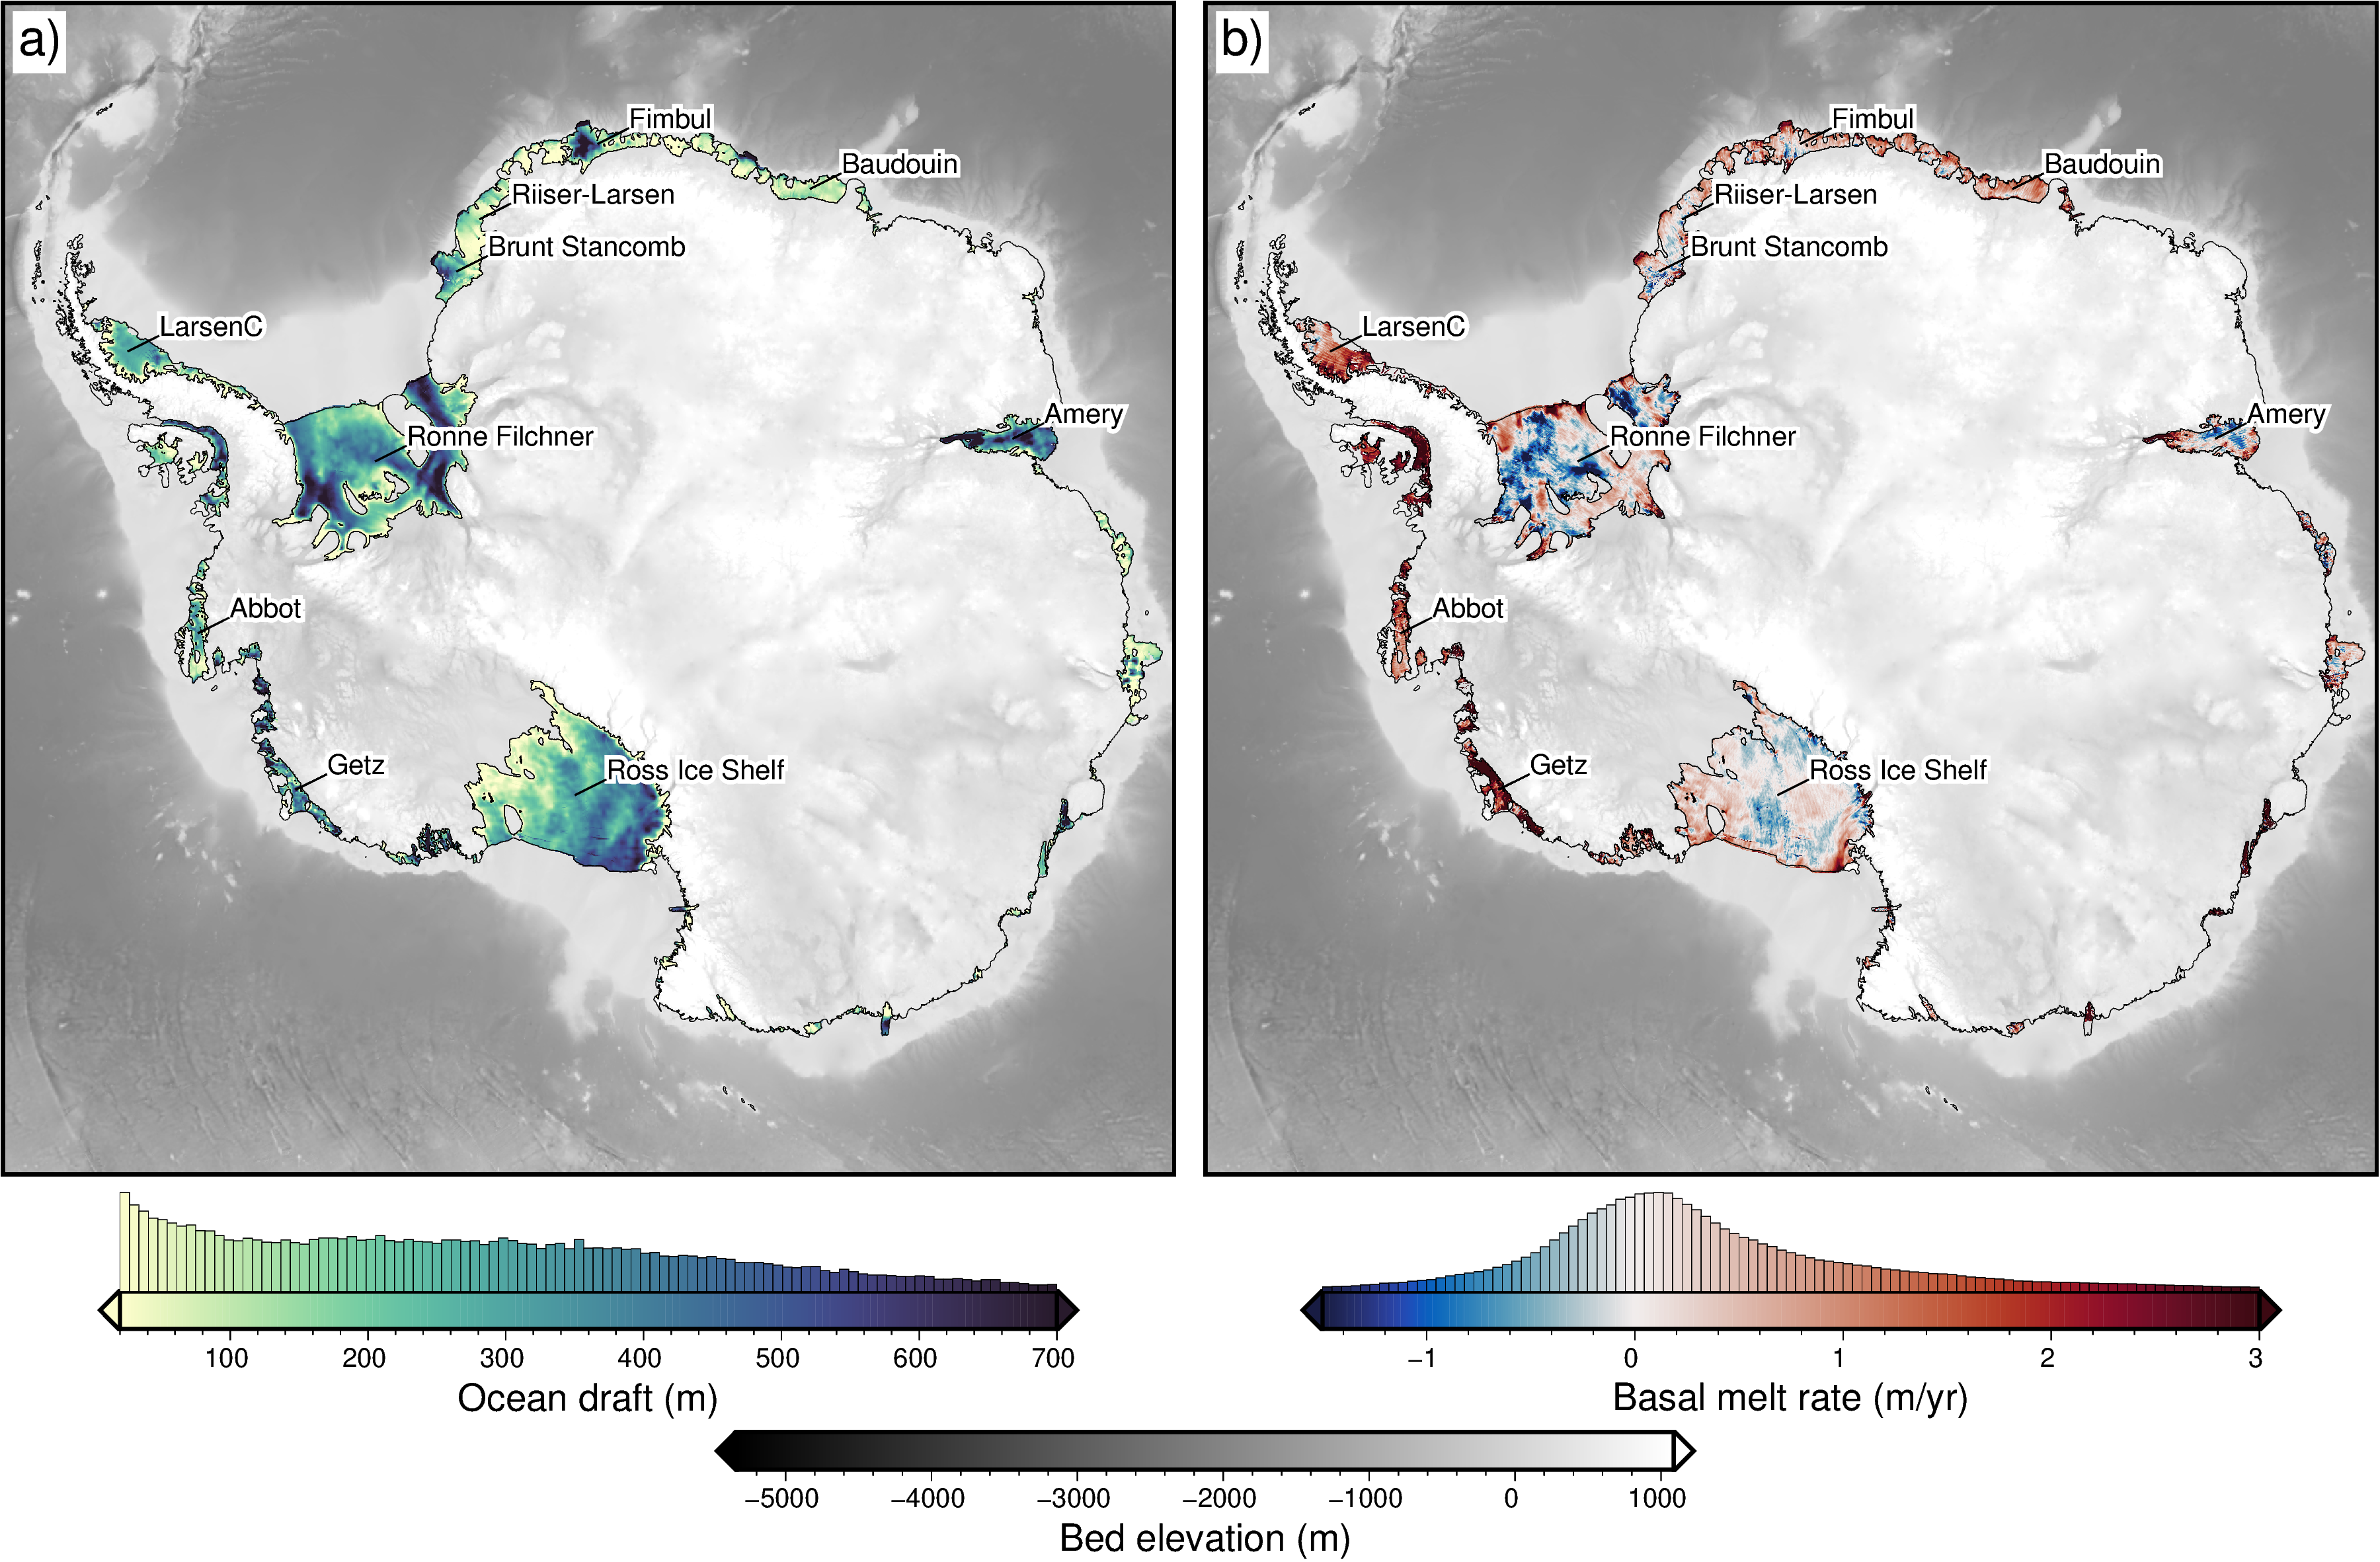
\includegraphics[width=0.95\textwidth]{figures/chp3/chp3_ice_shelves_basal_melt_and_ocean_draft.png}
    \caption[Ice shelves of Antarctica]{Ice shelves of Antarctica. \textbf{a)} Water column thickness beneath the ice shelves from Bedmachine data \citep{morlighemdeep2020, morlighemmeasures2022}. \textbf{b)} Basal melt rate for the ice shelves from \citet{adusumilliinterannual2020}. Both plots show bed elevations in the gray colormap. The 10 largest ice shelves are labelled.}
    \label{fig:chp3_ice_shelves}
\end{figure}

While the elevation of the ice base for many of Antarctica's ice shelves is relatively well-constrained, the water depth is poorly known. The relatively good understanding of the ice base comes from a combination of airborne radar surveys \citep[e.g.][]{dasmulti2020} and satellite altimetry measurements \citep[e.g.][]{griggsantarctic2011}, in conjunction with the hydrostatic equilibrium assumption \citep{bambercomparison1994}. Conversely, there is no equivalent fast and cheap technique to directly survey the bathymetry beneath floating ice shelves. Radar (ground or airborne) cannot image through the thick water, over-ice seismic surveys are slow and expensive, and numerous direct observations through drill holes are impractical. Due to the density contrast between the water and the sediment, the bathymetry surface produces a measurable gravity signal. This signal can be observed from airborne or ground-based gravity surveys, which provides a method, if used correctly, to model sub-shelf bathymetry. This method is a gravity inversion; a geophysical technique to take measurements of an energy source and estimate the physical properties responsible for these measurements \citep[e.g.,][]{oldenburginversion2005, tarantolainverse2005, menkegeophysical2012}. In this case, the energy source is Earth’s gravitational field and the physical Earth property is the depth of the density contrast between the ocean and seafloor. This chapter will first introduce the gravity inversion technique in general, followed by the specific style of gravity inversion, a geometric inversion, which is used here. Next, a suite of synthetic models will be used to assess the performance and limitations of the inversion. The suite of models includes:
\begin{enumerate}
    \item a simple synthetic topography.
    \item a synthetic topography with a regional component of the gravity signal.
    \item a semi-realistic model, using real Antarctic bathymetry and basement topographies to create the synthetic observed gravity. 
\end{enumerate}

With this suite of models, we will test the effects of various levels of noise, the data spacing of the observed gravity, the number of prior constraints, and various inversion methods and parameters. Finally, we will discuss the general limitations of using gravity inversions to recover bathymetry and will provide guidance for conducting gravity inversion for sub-ice-shelf bathymetry. 

\section{Methods}

There are two fundamental types of geophysical modelling, forward modelling, and inverse modelling. Forward modelling is the process of simulating observed data from a model of physical properties. For a gravity application, this may be calculating the gravitational field resulting from a sedimentary basin of a given geometry and/or density model. In general, forward problems are well-posed, meaning there is a unique answer \citep{oldenburginversion2005}. In contrast, inverse modelling, or inversion, is the process of determining physical properties from observed data. For the previous example, this would entail using observed gravity data to predict the sediment thickness of a basin. Inverse problems are generally ill-posed. For a given set of gravity observations, there is a multitude of sedimentary basin configurations which reproduce the observed data with the same degree of accuracy. This is referred to as non-uniqueness and makes geophysical inversions a difficult procedure compared to forward modelling.

\subsection{Geophysical inversion}

In general, inversions consist of three components;

\begin{enumerate}
    \item Forward operator ($f$): This is a mathematical means of linking a physical Earth property to the expected geophysical response. It accomplishes the task of forward modelling, as described above.
    \item Physical property model ($p$): This is a representation of the physical Earth property of interest. While real-world properties are continuous (i.e. a smoothly varying topography), computation often necessitates discretization (i.e. a DEM (digital elevation model), see section \ref{chp3_discretization}). The starting model ($p_0$) typically will include the prior geologic knowledge of the region. To discretize the topography we use a layer of adjacent, vertical right-rectangular prisms.
    \item Fit function ($\phi$): This function describes the similarity between the observed data and the predicted data (resulting from the forward calculation of the property model ($f(p)$)). The goal of the inversion is to minimize this function so that $f(p)$ is as close to the observed data as possible. 
\end{enumerate} 

Here, a mathematical derivation of a generalized discrete inversion problem is shown, following closely to the derivation of \citet{oliveiratopicos2014}. The inversion problem can be framed as finding the set of physical parameters ($\vv{p}$) which when modelled with the forward operator ($f$) produce predicted data ($\vv{d}^{pred}$) as close to the observed data ($\vv{d}^{obs}$), as possible. This inversion is discrete because the topography is represented with a series of grid cells, instead of a continuous function. The difference between the observed and predicted data gives the misfit $\vv{m}$, where 

\begin{equation} \label{eq:misfit}
    \vv{m} \quad = \quad \vv{d}^{obs} - \vv{d}^{pred} \quad = \quad \vv{d}^{obs} - \vv{f}(\vv{p}).
\end{equation}

Here, the $\ell^2$-norm (mean squared error) of the misfit is the metric used to define the \textit{closeness} between the predicted and observed data, where

\begin{equation}
    ||\vv{m}||_2 =  \sqrt{\sum_{i=1}^N [d_i^{obs} - \vv{f_i}(\vv{p})]^2},
\end{equation}

where $N$ is the number of observed data points.

This is defined as the \textit{fit function}, $\phi(\vv{p})$.  The fit function can also be expressed as

\begin{equation}\label{eq:fit_func}
    \phi(\vv{p}) \quad = \quad \vv{m}\cdot\vv{m} \quad = \quad [\vv{d}^{obs} - \vv{f}(\vv{p})]\cdot[\vv{d}^{obs} - \vv{f}(\vv{p})].
\end{equation}
% \begin{equation}\label{eq:fit_func}
%     \phi(\vv{p}) \quad = \quad \vv{m}\cdot\vv{m} \quad = \quad \vv{m}^T\vv{m} \quad = \quad [\vv{d}^{obs} - \vv{f}(\vv{p})]^T [\vv{d}^{obs} - \vv{f}(\vv{p})].
% \end{equation}

In this context, the inversion problem is to determine a vector of parameters $\tilde{p}$ of length $M$ which minimizes $\phi(\vv{p})$. This minimum occurs where the gradient of $\phi(\vv{p})$ at the vector $\tilde{p}$ has zero length.  The gradient of  $\phi(\vv{p})$ evaluated at any $\vv{p}$ is an M-dimensional vector is defined as 
\begin{equation}\label{eq:gradient}
    \nabla\phi(\vv{p}) = \left[\begin{array}{ccc}
    \dfrac{\partial \phi(\vv{p})}{\partial p_{1}}  \\
    \dfrac{\partial \phi(\vv{p})}{\partial p_{2}}  \\
    \vdots \\
    \dfrac{\partial \phi(\vv{p})}{\partial p_{M}} 
\end{array}\right].
\end{equation}

Evaluating the gradient at the i\textsuperscript{th} element, using Equation \ref{eq:fit_func} gives

\begin{equation} \label{eq:partial_deriv_phi}
\begin{aligned}
    \dfrac{\partial \phi(\vv{p})}{\partial p_i} &= 
    \dfrac{\partial}{\partial p_i} \sum_j{
    [d_j^{obs} - f_j(\vv{p})]\cdot[d_j^{obs} - f_j(\vv{p})]
    } \\
    &= \sum_j{\dfrac{\partial}{\partial p_i} 
    [d_j^{obs} - f_j(\vv{p})]\cdot[d_j^{obs} - f_j(\vv{p})]
    } \\
    &= -2\sum_j{\dfrac{\partial f_j(\vv{p})}{\partial p_i}\cdot[d_j^{obs} - f_j(\vv{p})]
    }
\end{aligned}
\end{equation}

Substituting Equation \ref{eq:partial_deriv_phi} into the elements of Equation \ref{eq:gradient} gives

% \begin{equation}
%     \nabla\phi(\vv{p}) = 
%      -2 [\vv{d}^{obs} - \vv{f}(\vv{p})] \times  
%      \left[\begin{array}{ccc}
%         \sum_j{\dfrac{\partial f_j(\vv{p})}{\partial p_1}}  \\
%         \vdots \\
%         \sum_j{\dfrac{\partial f_j(\vv{p})}{\partial p_M}} 
%     \end{array}\right]
% \end{equation}

\begin{equation}
    \nabla\phi(\vv{p}) = 
     -2 \mathbb{J}(\vv{p})  [\vv{d}^{obs} - \vv{f}(\vv{p})],
\end{equation}

\noindent
where $\vv{p}$ is the parameter vector of dimension $M$, $\vv{d}^{obs}$ is the observed data vector of dimension $N$ and $\mathbb{J}$ is the Jacobian matrix of dimension $M \times N$, and is given by

\begin{equation}
\mathbb{J}(\vv{p}) =
\begin{bmatrix}
    \dfrac{\partial f_1(\vv{p})}{\partial p_1} &
        \ldots &
        \dfrac{\partial f_N(\vv{p})}{\partial p_1}
    \\
    \vdots & \ddots & \vdots 
    \\
    \dfrac{\partial f_1(\vv{p})}{\partial p_M} &
        \ldots &
        \dfrac{\partial f_N(\vv{p})}{\partial p_M}
\end{bmatrix}
\label{eq:jacobian}
\end{equation}

Each element of the Jacobian matrix is given by

\begin{equation}
\mathbb{J}_{ij} =
    \dfrac{\partial f_j(\vv{p})}{\partial p_i},
% =
% \begin{bmatrix}
%     \dfrac{\partial f_1}{\partial p_1} &
%         \ldots &
%         \dfrac{\partial f_N}{\partial p_1}
%     \\
%     \vdots & \ddots & \vdots
%     \\
%     \dfrac{\partial f_1}{\partial p_M} &
%         \ldots &
%         \dfrac{\partial f_N}{\partial p_M}
% \end{bmatrix}
\label{eq:jacobian_element}
\end{equation}


% \begin{multline}
%     \dfrac{\partial \phi(\vv{p})}{\partial p_{i}} = 
%     \dfrac{\partial}{\partial p_{i}} \Big\{
%     [\vv{d}^{obs} - \vv{f}(\vv{p})]^T [\vv{d}^{obs} - \vv{f}(\vv{p})]
%     \Big\} \\
%     = 
%     \Bigg\{ -\dfrac{\partial \vv{f}(\vv{p})^T}{\partial p_{i}} [\vv{d}^{obs} - \vv{f}(\vv{p})] \Bigg\} +   
%     \Bigg\{ - [\vv{d}^{obs} - \vv{f}(\vv{p})]^T \dfrac{\partial \vv{f}(\vv{p})}{\partial p_{i}} 
%     \Bigg\} 
% \end{multline}
% which, since the transpose of a scalar is equal to itself, is simplified to

% \begin{equation}\label{eq:partial_deriv_phi}
%     \dfrac{\partial \phi(\vv{p})}{\partial p_{i}} = 
%      -2 \dfrac{\partial \vv{f}(\vv{p})^T}{\partial p_{i}} [\vv{d}^{obs} - \vv{f}(\vv{p})].
% \end{equation}

% Substituting Equation \ref{eq:partial_deriv_phi} into Equation  \ref{eq:gradient} and simplifying gives

% \begin{equation}
%     \nabla\phi(\vv{p}) = -2 \mathbb{J}(\vv{p})^T [\vv{d}^{obs} - \vv{f}(\vv{p})]
% \end{equation}

% where the matrix $\mathbb{J}(\vv{p})$ has dimensions $N \times M$ and is the \textit{Jacobian matrix} of  $\vv{f}(\vv{p})$.

% \begin{equation}
% \mathbb{J}(\vv{p}) =
% \begin{bmatrix}
%     \dfrac{\partial\vv{f}(\vv{p})}{\partial p_1} &
%     \dfrac{\partial\vv{f}(\vv{p})}{\partial p_2} &
%     \ldots &
%     \dfrac{\partial\vv{f}(\vv{p})}{\partial p_M}
% \end{bmatrix}
% =
% \begin{bmatrix}
%     \dfrac{\partial f_1(\vv{p})}{\partial p_1} &
%         \dfrac{\partial f_1(\vv{p})}{\partial p_2} &
%         \ldots &
%         \dfrac{\partial f_1(\vv{p})}{\partial p_M}
%     \\
%     \dfrac{\partial f_2(\vv{p})}{\partial p_1} &
%         \dfrac{\partial f_2(\vv{p})}{\partial p_2} &
%         \ldots &
%         \dfrac{\partial f_2(\vv{p})}{\partial p_M}
%     \\
%     \vdots & \vdots & \ddots & \vdots
%     \\
%     \dfrac{\partial f_N(\vv{p})}{\partial p_1} &
%         \dfrac{\partial f_N(\vv{p})}{\partial p_2} &
%         \ldots &
%         \dfrac{\partial f_N(\vv{p})}{\partial p_M}
% \end{bmatrix}.
% \label{eq:jacobian}
% \end{equation}

\noindent
which is the partial derivative of the j\textsuperscript{th} predicted data with respect to the i\textsuperscript{th} physical parameter. The \textit{Jacobian} ($\mathbb{J}$) is a sensitivity matrix that describes how much the predicted data changes for an infinitesimal change in the physical parameter. For example, let's consider the case of a gravity inversion attempting to recover the density of subsurface cubes. The model consists of 100 cubes, and there are 10 observation points. The Jacobian would be a $100 \times 10$ matrix where $\mathbb{J}_{1,1}$ (the first entry) would be the 1st cube's gravitational derivative with respect to density at the first observation point. The Jacobian, therefore, describes how sensitive each pair of cubes and observations are to a change in density. \\

Once the Jacobian is created, a matrix equation of the form $Ax=b$ is set up, where $A$ is the Jacobian, $x$ is the unknown variable, and $b$ is the data misfit.  
\begin{equation} \label{eq:matrix_eq}
    \mathbb{J} \vv{x} = \vv{m}
\end{equation}

A solution to this linear equation can be found directly, by finding the inverse or pseudo-inverse matrix of the Jacobian, or iteratively via a least-squares solver \citep{jacobygravity2009}. The solution gives the correction which when applied to the physical parameters of interest minimizes the misfit between the observed data and the starting model. 

\subsubsection{Non-Linear inversions}

The derivative of the forward operator with respect to the parameter of interest determines the linearity of an inversion. For a gravity inversion attempting to recover rock density, the derivative of gravity with respect to density is constant, and thus the inversion is considered linear \citep{asterparameter2018}. Conversely, a gravity inversion attempting to recover the depth to a surface, or the thickness of a layer, is non-linear since the vertical derivative of gravity (derivative with respect to depth) is dependent on the depth. Non-linear inversion cannot be solved directly, with matrix inversion \citep{jacobygravity2009}. They must be linearized; which is the purpose of the Jacobian matrix. The Jacobian enables a minimum-norm solution to be found with an iterative solver, where at each iteration, the calculated corrections ($\vv{x}$) are applied to the starting model, the residuals ($\vv{m}$) are recalculated, the Jacobian is updated, and Equation \ref{eq:matrix_eq} is solved again, giving a new set of corrections. This is repeated until $\phi(\vv{p})$ is suitably low.

\subsubsection{Geometric inversions}
Most gravity inversions aim to recover the distributions of densities in the subsurface. For this technique, the model domain is discretized into a series of polygons (for 2D) or polyhedrons (for 3D), and the inversion aims to predict the density of each polygon. This is widely used due to its relevance in mineral exploration \citep{oldenburggeophysical2007}. Less commonly used are gravity inversions which aim to recover the depth, shape, or volume of features. This style of gravity inversions are referred to as geometric inversions. They are typically used to estimate relief of the Moho \citep[e.g][]{uiedafast2017, borghimoho2022} or the sediment-basement contact \citep[e.g.][]{santosefficient2015, barbosagravity2007}. In this chapter, geometric inversions are used to recover the bathymetry. This use case of gravity inversion is unique to studying the cryosphere. In locations without ice cover, bathymetry data is typically collected with shipborne multi-beam echo sounding, airborne LiDAR, or satellite altimetry. 

\subsection{Forward modelling}

To perform a geometric gravity inversion, first, the gravitational field produced by a topographic surface must be able to be calculated. This topography is approximated as a constant density contrast between the overlying and underlying materials. The topography is often modelled as a series of adjacent vertical right-rectangular prisms. For a certain observation point, the gravitational field produced by this layer of prisms is the sum of the forward gravity of each prism. This forward gravity calculation of a prism is accomplished with the analytical solutions given by \citet{nagygravitational2000}, as implemented in the Python package Harmonica \citep{fatiandoaterraprojectharmonica2023}.

\subsubsection{Discretization}\label{chp3_discretization}
There are several options for discretizing a density contrast as a series of prisms (Figure \ref{fig:chp3_discretization}). The most conceptually simple method is for the prisms to represent the true density and geometry of the material on either side of the surface (Figure \ref{fig:chp3_discretization}b). In this method, the topography is represented by the base of the upper prisms, and by the tops of the lower prisms. Alternatively, the contrast can be represented by a layer of prisms either above or below the surface, ending at an arbitrary reference, typically the minimum or maximum value of the surface (Figure \ref{fig:chp3_discretization}c-d). For this, the prism’s density values are relative to the medium on the other side of the surface (i.e. if prisms are below the surface, their densities are $\rho_{below} - \rho_{above}$). The last option is to choose a flat reference surface (typically the mean value of the surface or sea level) and create prisms between this and the surface (Figure \ref{fig:chp3_discretization}e). Prisms above the reference are assigned a positive density contrast ($\Delta{\rho} = \rho_{below} − \rho_{above}$), and prisms below the surface a negative density contrast ($\Delta{\rho} = \rho_{above} − \rho_{below}$). All of these methods result in similar forward gravity calculations. Note that the absolute density option (Figure \ref{fig:chp3_discretization}b) has twice as many prisms as the other options, significantly increasing its computational expense, regardless of whether or not a buffer zone is used.

\begin{figure}[!ht]
    \centering
    \includesvg[inkscapelatex=false,width=0.65\textwidth]{chp3/chp3_discretization}
    \caption[Equivalent methods of discretizing a density contrast]{Equivalent methods of discretizing a density contrast (\textbf{a}) across a surface. \textbf{b)} Use absolute densities of the mediums above and below the reference, with prisms on either side. \textbf{c-d)} Use the density contrast across the surface, with prisms either above or below, and the sign of the density contrast reflecting whether they are above or below. \textbf{e)} Use a reference surface, with prisms above having a positive density contrast and prisms below a negative contrast.}
    \label{fig:chp3_discretization}
\end{figure}

\subsubsection{Gravity edge effects} \label{chp3_edge_effects}
Any forward gravity calculation of a surface will include gravitational edge effects. These effects are typically a decay in the gravitational field towards the edges of the prism model due to the void space (density of 0) beyond the edge of the model. The magnitude of decay is dependent on the average thickness and density of prisms near the edge. Larger or denser prisms create a large contrast with the void space, resulting in a greater amount of decay. Therefore, the absolute density method of discretization (Figure \ref{fig:chp3_discretization}b) produces the largest edge effects due to the high-density values and large total thickness of the prisms. The relative density methods (Figure \ref{fig:chp3_discretization}c-d) produce a smaller edge effect, since the prisms are only above or below the surface, reducing their total thickness. The density values are also less than in the absolute density method. The reference surface method (Figure \ref{fig:chp3_discretization}e) produces the smallest edge effects due to both a) the mean prism thickness being smaller, and b) positive and negative density prisms having opposite edge effects, partially cancelling each other out. This is only applicable if the reference level is located within the range of the values of the surface. Note that with a reference level completely above or below the surface, the reference method becomes identical to methods c) and d) of Figure \ref{fig:chp3_discretization}. \\

A buffer zone can be used to reduce the impact of these edge effects by calculating forward gravity confined to an inner region, while the prism model extends beyond. This limits the majority of the edge effects to outside the region of calculation. Too large of a buffer zone will add an unnecessary amount of computation (more prisms), while too small of a zone will introduce unacceptably large edge effects to the calculations.


\subsection{Isolating anomalies}

For a successful geometric gravity inversion, the component of the observed gravity field resulting from the density contrast of interest must be isolated from all other gravity signals. This section describes the process of isolating the required anomaly. Since this chapter consists of synthetic gravity, the discussion of correcting raw gravity measurements and deriving the various gravity anomalies is omitted. See Chapter \ref{ch:4} for further discussion of gravity data processing. Here, \textit{synthetic observed gravity} is taken to mean the gravity effect resulting solely from deviations between the true synthetic model, and a simple reference model, defined by a flat surface with a constant density above and a constant density below. This is considered a partial topo-corrected gravity disturbance, since the gravity effect of other layers, such as ice and water, if present, is assumed to have been corrected for. The misfit, $\vv{m}$, in Equation \ref{eq:misfit}, is defined as this synthetic observed gravity minus the forward gravity effect of the starting bathymetry. \\

\subsection{Regional vs. Residual gravity} \label{chp3_regional_seperation}

The topography-free gravity disturbance is often simplified as consisting of two components, the regional and residual fields. The regional field typically dominates the signal and is often the result of deeper and broader structures, such as Moho variations. Superimposed on this signal is the residual field, which is typically the result of shallower structures. The terms residual and regional are relative; here, they are taken to mean the gravity effect of the bathymetry versus that of all deeper structures, respectively. In this inversion, the residual, regional, and misfit are related by

\begin{equation} \label{eq:regional_residual}
    \vv{m} = \vv{m}_{res} + \vv{m}_{reg},
\end{equation}

\noindent
where $\vv{m}$ is the overall data misfit, from Equation \ref{eq:misfit}. The residual misfit, $\vv{m}_{res}$, is the desired input into the inversion, and thus the regional component, $\vv{m}_{reg}$, must be removed prior to the inversion. This step proves to be one of the most challenging steps of a bathymetric inversion, especially in areas of limited constraints \citep{brisbourneseabed2014}. Removing an incorrect regional field, whether it is too much or too little, will directly impact the resulting bathymetry results. Regional-residual separation is also highly non-unique and benefits greatly from \textit{a priori} constraints. Many methods of regional separation rely on the simplifying assumption that the regional field consists of longer-wavelength anomalies, while the residual field dominates the short-wavelength components. Here, four methods of estimating the regional component of gravity are described.

\begin{enumerate}
    \item Low-pass filter:
        With the assumption outlined above, a low-pass filter can be used to isolate the regional gravity. For this, a Gaussian wavelength filter is used and the filter width can be varied based on the expected regional anomaly wavelengths. This method requires the data to be gridded over the entire domain, which may be a problem for sparse surveys. or irregularly shaped domains. The choice of wavelength is subjective and needs to be carefully considered. See \citet{eisermannbathymetry2020} for a bathymetry inversion utilizing this method of regional separation. 
    \item Trend removal:
        Similar to the low-pass filter method, a trend can be fit to the misfit data, representing the regional field. The order of the polynomial trend is subjective and can be varied to suit the data. Again, this parameter choice requires care.
    \item Equivalent source prediction:
        The equivalent sources technique is a method commonly used to grid, smooth, or upward-continue gravity data. It creates a set of point sources with densities, which when forward-modelled, reproduce the measured gravity data. These sources are then used to predict the gravity anomaly at any desired point. The source depths can be varied to achieve the desired regional component. This technique is beneficial over low-pass filter and trend removal in that it does not require the data to be gridded and can thus accommodate sparse surveys, or compilations of surveys at varying altitudes. It is computationally expensive compared to the above methods. Additionally, source depths are a subjective parameter, which needs to be carefully chosen. Past bathymetry inversions have used upward continuation as a means to define the regional field \citep[e.g.,][]{tintobathymetry2015}.
    \item Constraint point minimization:
        The last method makes use of constraint points where the bathymetry depths are known. This inversion defines the residual component of the misfit as the gravity effect from deviations of the true bathymetry with respect to the starting bathymetry. At constrained points, there is no deviation between the starting and true bathymetries, and thus the residual component of the misfit should be zero at the constraints. This means the total misfit value at the constrained points is equal to the regional component (Equation \ref{eq:regional_residual}). By sampling the misfit at each constrained point, and fitting a surface to these values, a regional component is estimated. This technique has a few advantages. It imposes a form of smallness regularization, where the inversion won't significantly alter the depth of the constraint points since the input residual at the points is $\sim$0~mGal. Additionally, except for the gridding technique, this method doesn't require a subjective parameter, unlike the other methods. Similar to the low-pass filter and trend removal, this method requires gridded data. If this data is sparse, or the constrained points are not located near gravity observation points, some inaccuracies will be introduced. This technique has been used in several bathymetry inversions \citep{millanconstraining2020, yangbathymetry2021, anbathymetry2019}.
        
\end{enumerate}

Other methods used to approximate the regional component include using high-altitude (satellite) gravity data \citep{mutosubglacial2016, tintobathymetry2015}, the forward modelling of a geologic model, either inferred from 1) other geophysical data \citep{hodgsonfuture2019}, 2) \textit{a priori} geologic knowledge \citep{tintoprogressive2011}, or 3) from an approximated crustal density distribution \citep{tintoross2019, cochrandetailed2020}. Once estimated, the regional component is then removed from the total misfit, giving the residual misfit. This residual misfit ideally results solely from discrepancies between the starting and true bathymetries. 

\subsection{Running the inversion}

Here, the necessary steps for running an inversion are explained. First, the Jacobian matrix is calculated (Equation \ref{eq:jacobian}). Next, the matrix equation (Equation \ref{eq:matrix_eq}) is solved, giving the necessary corrections to apply to the bathymetry. Additionally, this solution needs to be constrained to account for the inherent non-uniqueness of the inversion. This is accomplished with various forms of regularization; i.e., a unique solution is determined subject to minimize an additional objective function.

\subsubsection{Jacobian matrix} \label{chp3:jacobian_methods}

The first step of the inversion is to calculate the sensitivity matrix, the Jacobian (Equation \ref{eq:jacobian}). Each entry of the Jacobian (Equation \ref{eq:jacobian_element}) is the vertical derivative of gravity of a prism relative to a single observation point. While a solution exists to the analytical vertical gravity derivative of a prism, we use an approximation to limit the computational expense \citep{nagygravitational2000}. Here two methods are derived for approximating the vertical gravity derivative resulting from a prism; 1) an annular approximation and 2) a finite differences approach.

\paragraph*{Annulus approximation}

\begin{figure}[!ht]
  \centering
  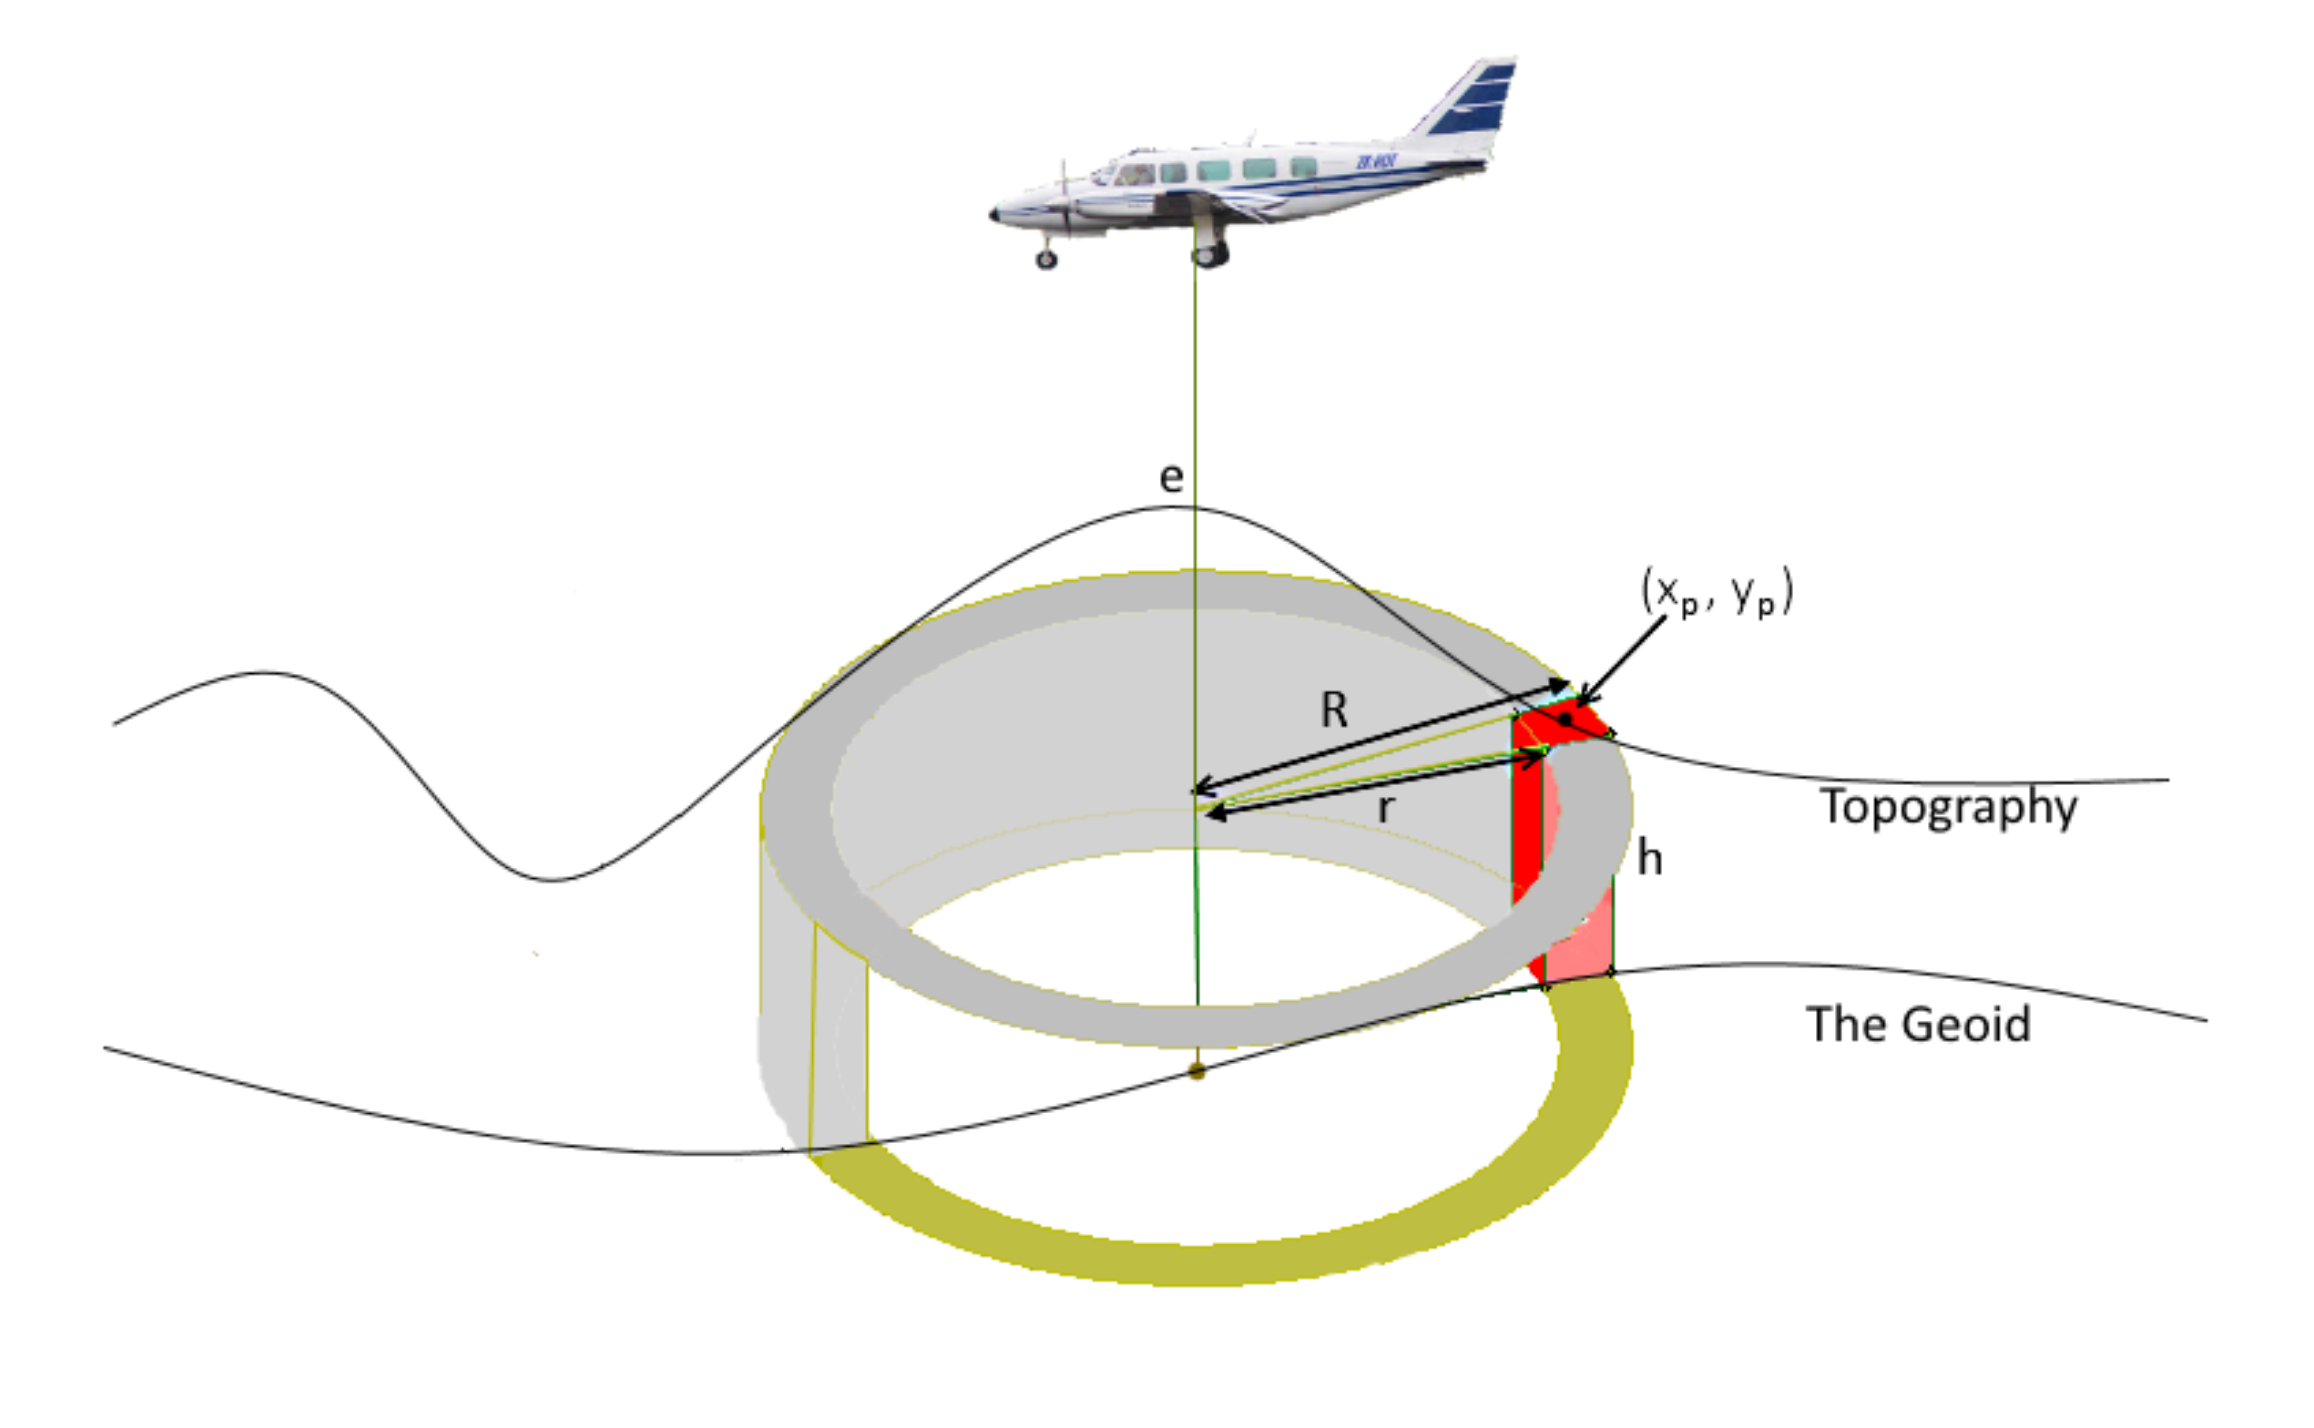
\includegraphics[width=0.7\linewidth]{figures/chp3/chp3_annulus.png}
  \caption[Annulus approximation of a vertical prism]{
    An illustration of an annulus of topography as an approximation for a vertical prism. From \citet{mccubbineairborne2016}.
  }
  \label{fig:chp3_annulus}
\end{figure}

A vertical prism can be approximated as a sector of an annulus (a cylindrical shell), as in Figure \ref{fig:chp3_annulus}. This approximation greatly simplifies the calculation of the vertical derivative of the prisms' gravity. The vertical component of gravity of an entire annulus (grey hollow cylinder in Figure \ref{fig:chp3_annulus}) is defined by

\begin{equation} \label{eq:annulus_gravity}
\delta g = 2 \pi G \rho (R - r + \sqrt{r^2 + h^2} - \sqrt{R^2 + h^2)}
\end{equation}

\noindent
where $\rho$ is the density, $G$ is the gravitational constant, $r$ and $R$ are the inner and outer radii, respectively, and $h$ is the average height of the cylinder \citep{hammerterrain1939}. $r$, $R$, and $h$ are relative to the observation point, located in the centre bottom of the annulus. \citet{mccubbineairborne2016} provides an adaption of Equation \ref{eq:annulus_gravity} which isolates the gravity of just a portion of this annulus (red section in Figure~\ref{fig:chp3_annulus}). This is accomplished by adding an additional factor $f$, relating the area of the annulus to the area of a sector of it:

\begin{equation}
f = \frac{\alpha^2}{\pi(R^2 - r^2)}
\end{equation}

\noindent
where

\begin{equation}
r = \sqrt{x^2+y^2} - \sqrt{\frac{\alpha^2}{2}}
\end{equation}

\begin{equation}
R = \sqrt{x^2+y^2} + \sqrt{\frac{\alpha^2}{2}}
\end{equation}

\noindent
where $\alpha$ is the prism width, $x$, $y$, and $z$ are coordinates of the prism centre, relative to the observation point. This factor $f$ is then multiplied by Equation~\ref{eq:annulus_gravity} to give the vertical component of gravity for a section of an annulus, $\delta g_{annulus} = f \delta g$.

Taking the derivative of this with respect to h gives

\begin{equation} \label{eq:vertical_derivative_annulus}
\dfrac{\partial g}{\partial h} = 2 f \pi G \rho h ( 
    \dfrac{1}{\sqrt{r^2 + h^2}} - \dfrac{1}{\sqrt{R^2 + h^2}} ).
\end{equation}

While the approximation of a prism as a section of an annulus introduces some errors, the calculation is efficient and simple to implement.

\paragraph*{Finite differences approximation}

Another option to calculate the vertical derivative for the Jacobian matrix is with numerical differentiation. For this, a small prism is added above each existing prism, its forward gravity is calculated and the result is divided by the small prism's height. This approximates the vertical derivative of gravity at the surface of the prism, relative to the observation point. \\

Both methods adequately determine the Jacobian. The annulus method is a more simple calculation and is thus faster, but is likely less accurate and introduces singularities. These singularities occur if the prism is directly beneath the observation point, so that either the inner or outer radii are negative (Figure \ref{fig:chp3_annulus}). These singularities are resolved by shifting the observation point to a prism edge. Conversely, the finite differences method, while it is a numerical approximation, uses analytical solutions for calculating the forward gravity \citep{nagygravitational2000, fatiandoaterraprojectharmonica2023}, and thus is valid in the entire domain, with no singularities. This increased robustness makes the computation slower. Section \ref{chp3_annulus_vs_prisms} compares the effectiveness and computation time of both of these methods.

\subsubsection{Least-squares solver}

With the Jacobian matrix and the vector of gravity residuals, Equation \ref{eq:matrix_eq} can be solved to find the set of surface correction values that minimize the fit function. Here, the matrix equation $\mathbb{J} \vv{x} = \vv{r}$ is solved with an iterative damped least squares algorithm \citep[LSQR][]{paigelsqr1982}. The algorithm gives the minimum-norm solution, where for a set of solutions that each fit the data with the same accuracy, the solution with the minimum $||p||^2$ is chosen. LSQR accepts a damping parameter, which helps regularize the problem, preventing the solution from becoming too large. The choice of the damping value is important as it directly affects the inverted results. The optimal value can be chosen with a cross-validation routine following that of \citet{uiedafast2017}, as described below.

\subsubsection{Regularization} \label{chp3:regularization}

Regularization is a series of techniques used to help constrain ill-posed inversion problems \citep{asterparameter2018}. Most potential field inversions, due to their inherent non-uniqueness, are ill-posed, containing many solutions which equally satisfy the data. Here regularization is split into \textit{smallness} and \textit{smoothness}. \textit{Smallness} deals with adhering to \textit{a priori} constraints, i.e. having the inverted surface elevation match the previous bathymetry measurements (constraint points). \textit{Smoothness} helps to achieve realistic topographic results, without major jumps or excessively steep slopes. 

\paragraph*{Smoothness}
To achieve a form of smoothness regularization, damping is applied at each iteration to the solver of the matrix equation. One method to choose an optimal damping value is cross-validation of the input gravity data \citep{uiedafast2017}. An effective inversion should produce a topography that, when forward-modelled, accurately recreates observed gravity data that weren't included in the inversion. This idea is the basis of the cross-validation routine. The observed gravity data is split into two sets, a \textit{training} and a \textit{testing} set. For an individual damping value, the inversion is run using only the training set. The final inverted bathymetry is then forward-modelled onto the observation points of the testing set. The difference between the observed and forward gravity at these testing points is calculated. The root mean square (RMS) of the differences provides a metric for the effectiveness of the damping; this is referred to as the \textit{score}. This process is then repeated for a suite of damping values, and the value which produces the lowest score is used as the optimal damping value. In this inversion, the gravity data, whether they are airborne flight lines or scattered ground stations, are interpolated onto a regular grid (see Section \ref{chp3:eq source resampled}). To create the testing set of observed gravity data, the original data are interpolated onto a grid at half the desired grid spacing. This leaves the training set with the desired number of points. This grid spacing configuration is shown in Figure \ref{fig:chp3_CV_grid_spacing}.

\begin{figure}[!ht]
    \centering
    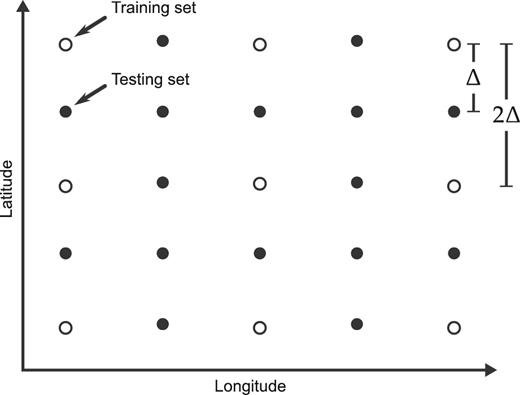
\includegraphics[width=0.5\textwidth]{figures/chp3/chp3_CV_grid_spacing.jpg}
    \caption[Training and testing set configuration]{Configuration of observed gravity data observation points, split into training and testing sets. Reprinted from \citet{uiedafast2017}.}
    \label{fig:chp3_CV_grid_spacing}
\end{figure}

\paragraph*{Smallness}
A form of smallness regularization is applied here to ensure the inversion results adhere to any \textit{a priori} bathymetry constraints. A portion of this smallness regularization is already accounted for when using the constraint point minimization method of regional-residual separation. This method minimizes the residual component of the gravity misfit at the constraint points by assigning the majority of the misfit to the regional component. However, non-zero residual values near the constraints will result in a non-zero correction of the prisms immediately surrounding the constraint. For further smallness regularization, a weighting grid (Figure \ref{fig:chp3_simple_weights}) is used to ensure the surface correction values at each iteration are 0 at constraint points. If only the prism immediately at the constraint point is fixed, a \textit{pedestal} effect commonly develops. This is where the nearby prisms' surfaces freely move during the inversion, yet the constrained prism is fixed, resulting in either a pedestal or a hole. To avoid this, the weighting grid smoothly decays from a value of 0 at the constraints, to a value of 1 at a distance. To create this grid, the minimum distance between each grid cell (prism) and the nearest constraint point is calculated. These values are then normalized from 0 to 1 (Figure \ref{fig:chp3_simple_weights}). At each iteration, the least squares solver yields a grid of surface correction values. Before being added to the prism layer, the grid is multiplied by this weighting grid. This results in surface corrections of 0 for prisms located at constraint points, unmodified surface correction values far from constraint points, and a smooth taper between these two endmembers. \\

\begin{figure}[!ht]
    \centering
    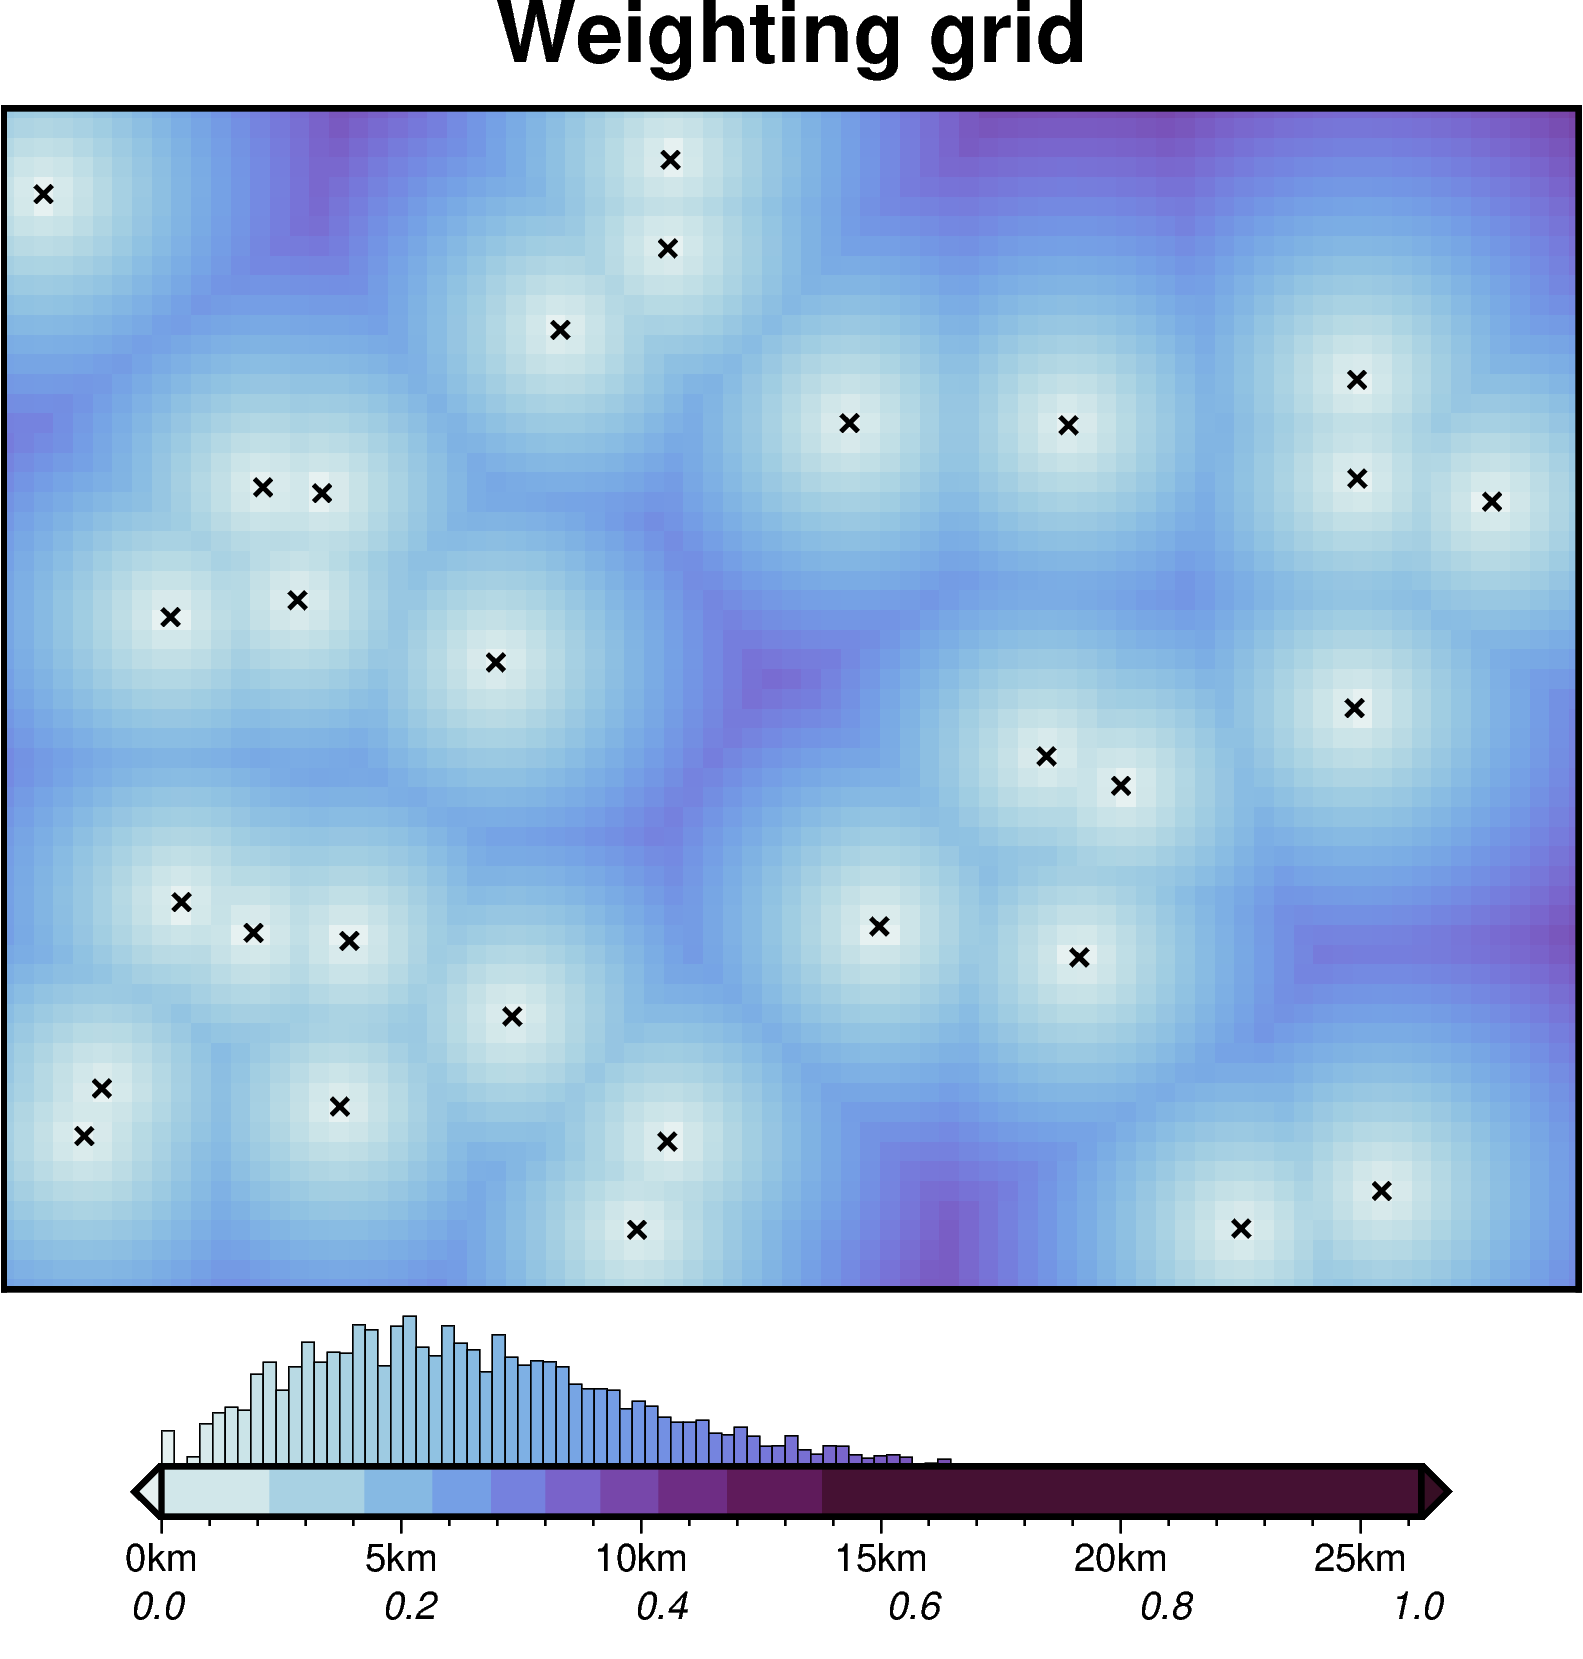
\includegraphics[width=0.5\textwidth]{chp3/chp3_simple_weights}
    \caption[Weighting grid for the simple synthetic inversion]{Weighting grid for the simple synthetic inversion, created from the minimum distance between each grid cell and the nearest constraint (black crosses). Grid values are normalized from 0 to 1 to produce the weighting grid (lower colourmap annotations).}
    \label{fig:chp3_simple_weights}
\end{figure}

The above sections outline a single iteration of the inversion. Once the surface correction is calculated and the weights are applied, these values are added to the starting bathymetry (or the last iterations inverted bathymetry). This is then re-discretized into prisms. The updated prisms are then forward modelled to create a new predicted gravity, $\vv{d}^{pred}$. This is subtracted from the observed gravity, $\vv{d}^{pred}$, to get a new misfit, $\vv{m}$. Using the same original regional component, the updated residual gravity misfit, $\vv{m}_{res}$, is calculated. This is now the input into the second iteration of the inversion. This process is repeated until a user-determined termination. Next, we outline the four criteria for ending the inversion. 

\subsection{Stopping Criteria} \label{chp3:stopping_criteria}

The inversion is terminated on one of four stopping criteria:

\begin{enumerate}
    \item when the inversion reaches a maximum number of iterations ($N$)
    \item when the $\ell^2$-norm of the residual ($||\vv{m}||_2$, Equation \ref{eq:misfit}) is less then a set $\ell^2$-norm tolerance
    \item if there is no significant variation in the $\ell^2$-norm between iterations (i.e. the $\Delta||\vv{m}||_2$ is less than a set tolerance)
    \item if the $\ell^2$-norm increases above a certain threshold of the starting $\ell^2$-norm. 
\end{enumerate}
The maximum number of iterations is set as a safety margin to avoid excessively long-running inversions. The $\ell^2$-norm tolerance is used to end the inversion before excessive over-fitting of noise in the data. This should be set to the square root of the assumed noise level of the gravity data. The $\Delta\ell$2-norm tolerance is used to end inversions that have reached their limit of reducing the $\ell^2$-norm, Finally, the upper limit of $\ell^2$-norm terminates run-away inversions, which occurred during the development of the inversion due to coding errors but is retained here as a fail-safe. 

\subsection{Software implementation}

The inversion algorithm described here is implemented within the Python programming language. The algorithm uses many open-source scientific libraries. These include Harmonica for the forward gravity modelling of prisms and equivalent sources calculations \citep{fatiandoaterraprojectharmonica2023, solergradientboosted2021}, Verde for various spatial operations \citep{uiedaverde2018}, PyGMT and Antarctic-Plots for figure creation \citep{uiedapygmt2021, tankersleyantarctic2023}, Scipy for least squares regression \citep{2020SciPy-NMeth}, and Optuna for hyperparameter optimization \citep{akibaoptuna2019}. The majority of the experiments were run in Jupyter notebooks \citep{pérezipython2007}, which are documented to explain the details of using the software. All source code, results, and figures involved in this chapter are made available in an online GitHub repository (\url{https://github.com/mdtanker/RIS_gravity_inversion}). See Section \ref{chp1_open_source} for the hardware used in this study.

\section{Synthetic models}
To assess the performance of the inversion and showcase its use, it is applied to a suite of synthetic test models. Each model has three components; 1) the `true' bathymetry surface, which the inversion is expected to model, 2) the `observed' gravity data, and 3) the `starting' bathymetry model, which is a low-resolution version of the true surface. The only inputs into the inversions are the observed gravity data and the starting bathymetry. The true bathymetry is only used to evaluate the performance of each inversion. The observed gravity data contains the forward gravity calculated from the true bathymetry, plus, in some cases, additional noise and other gravity signals such as a regional field. The starting bathymetry is created by sampling the true bathymetry at a set of points. These values are then used to re-grid the data for the entire region using a bi-harmonic spline interpolator \citep{uiedaverde2018}. This simulates the bathymetric knowledge of many ice shelves, where few direct measurements of bathymetry exist, such as drill holes, or single-point seismic surveys. These points are referred to as the constraints. The models tested here include:
\begin{enumerate}
    \item A simple model (Section \ref{chp3:simple_model}): This model sets a baseline performance expectation of the inversion, with no noise, dense gravity observation points, and no additional components included in the observed gravity. The synthetic bathymetry is created with Gaussian functions of various amplitudes and wavelengths. With this same simple model, the observed gravity data is re-gridded at a lower resolution, and random noise is added, to better simulate a gravity survey.
    \item A simple model with a regional field (Section \ref{chp3:simple_regional_model}): Using the same model as above, a `regional' component of the gravity field is added to the observed data.
    \item A semi-realistic model (Section \ref{chp3:Ross_Sea}): This last model is created from real bathymetry data from Antarctica's Ross Sea. This model tests the inversion's capabilities with more realistic bathymetric features expected for sub-ice-shelf environments.
\end{enumerate} 

\subsection{Simple model}\label{chp3:simple_model}

 \begin{figure}[!ht]
    \centering
    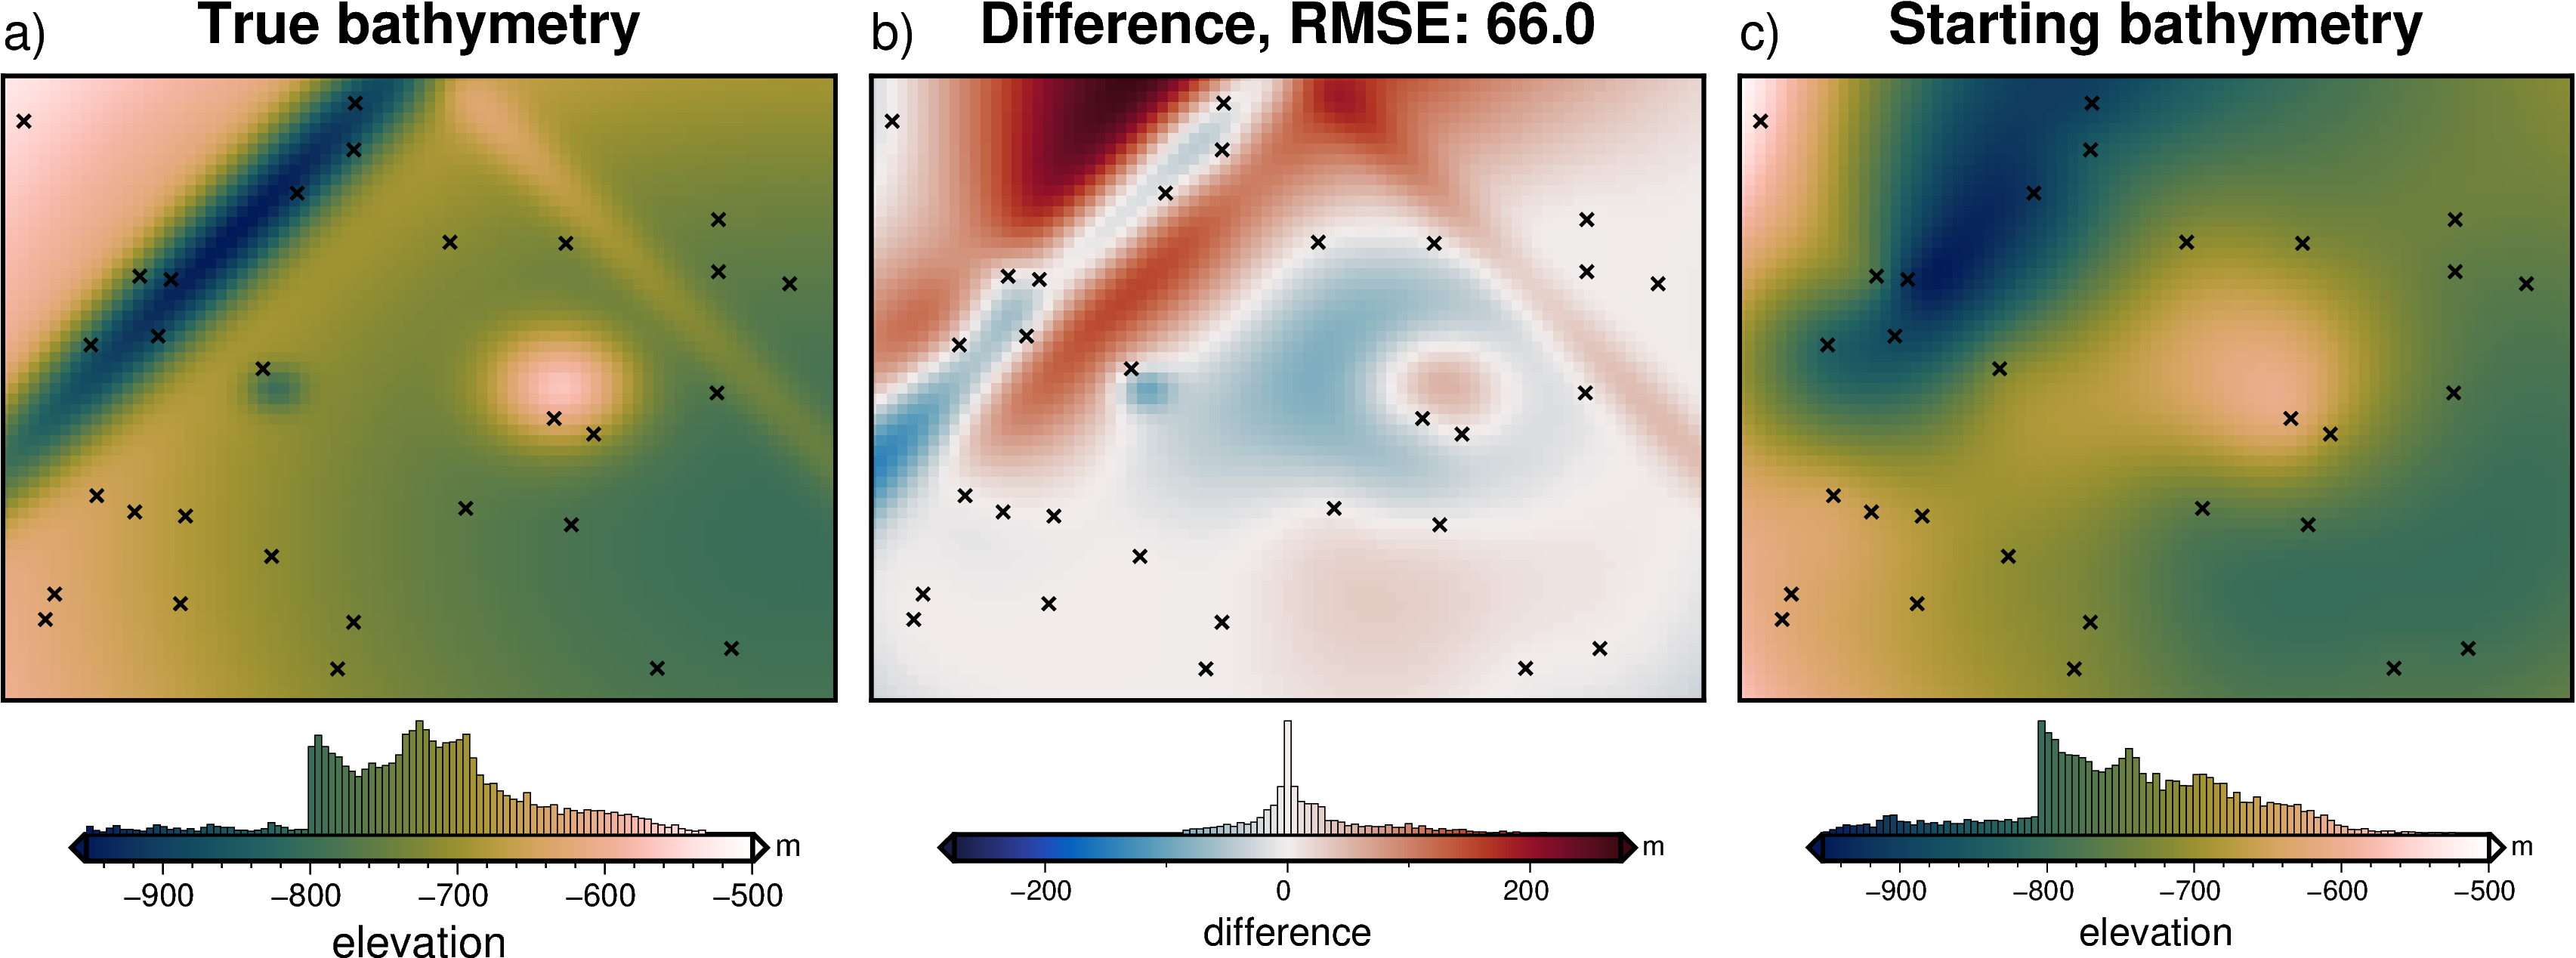
\includegraphics[width=0.95\textwidth]{chp3/chp3_simple_starting_model}
    \caption[Simple synthetic model bathymetry]{Simple synthetic model bathymetry. \textbf{a)} True bathymetry created from Gaussian functions, \textbf{b)} difference between a and c, and \textbf{c)} starting bathymetry, created from the sampling and re-gridding of the true bathymetry at 30 points (black crosses).}
    \label{fig:chp3_simple_starting_model}
\end{figure}

\subsubsection{Model setup}
Simulating typical sub-ice-shelf bathymetry, this model (Figure \ref{fig:chp3_simple_starting_model}a) has an average elevation of $\sim$ -700~m and ranges between $\sim$ -400~m and $\sim$ -1000~m. It contains features of various wavelengths, amplitudes, and shapes; namely two circular features and two linear features. Overall, the grid is eastward deepening and contains a shallow and wide E-W trough through the centre. The model domain is 80~x~60~km, with 1~km grid cells (4800 cells). A 6~km buffer zone in all directions was included to limit gravitational edge effects. 30 randomly located constraint points were used to create the starting bathymetry (Figure \ref{fig:chp3_simple_starting_model}c). The starting bathymetry has an RMS difference with the true bathymetry of 66~m. \\

To forward model the gravity of the true bathymetry, a layer of adjacent vertical right-rectangular prisms was created using the reference discretization method (Figure \ref{fig:chp3_discretization}e) with the mean elevation as the reference level. A density contrast of $\Delta\rho$ = 1276~kg~m\textsuperscript{-1} (contrast between seawater(1024~k~ m\textsuperscript{-1}) and sediment (2300~kg~m\textsuperscript{-1})), was used, with $+\Delta\rho$ for prisms above the reference, and $-\Delta\rho$ for prisms below the reference. The forward gravity of this prism layer was calculated at a constant height of 1000~m (roughly 1700~m above the bathymetry) on a regular grid at half the grid spacing (500~m) of the bathymetry. This represents the observed gravity data (Figure \ref{fig:chp3_simple_misfit}a) and consists of both the training and testing data sets used for the cross-validation (Section \ref{chp3:regularization}, Figure \ref{fig:chp3_CV_grid_spacing}). \\

The low-resolution starting layer was discretized in the same method, and the same density contrast was used. The forward gravity of these starting layer prisms results in the predicted gravity (Figure \ref{fig:chp3_simple_misfit}c). To account for any offset between the observed and predicted data, the observed data is DC-shifted to minimize the differences at the constraint points. The difference between the shifted observed and the predicted data gives the gravity misfit (Figure \ref{fig:chp3_simple_misfit}b). Since there is no regional component in this synthetic model, the input into the inversion, the residual misfit, is equal to this total misfit (Equation \ref{eq:regional_residual}). This residual misfit describes the ability of the starting model to predict the observed data. 

\begin{figure}[!ht]
    \centering
    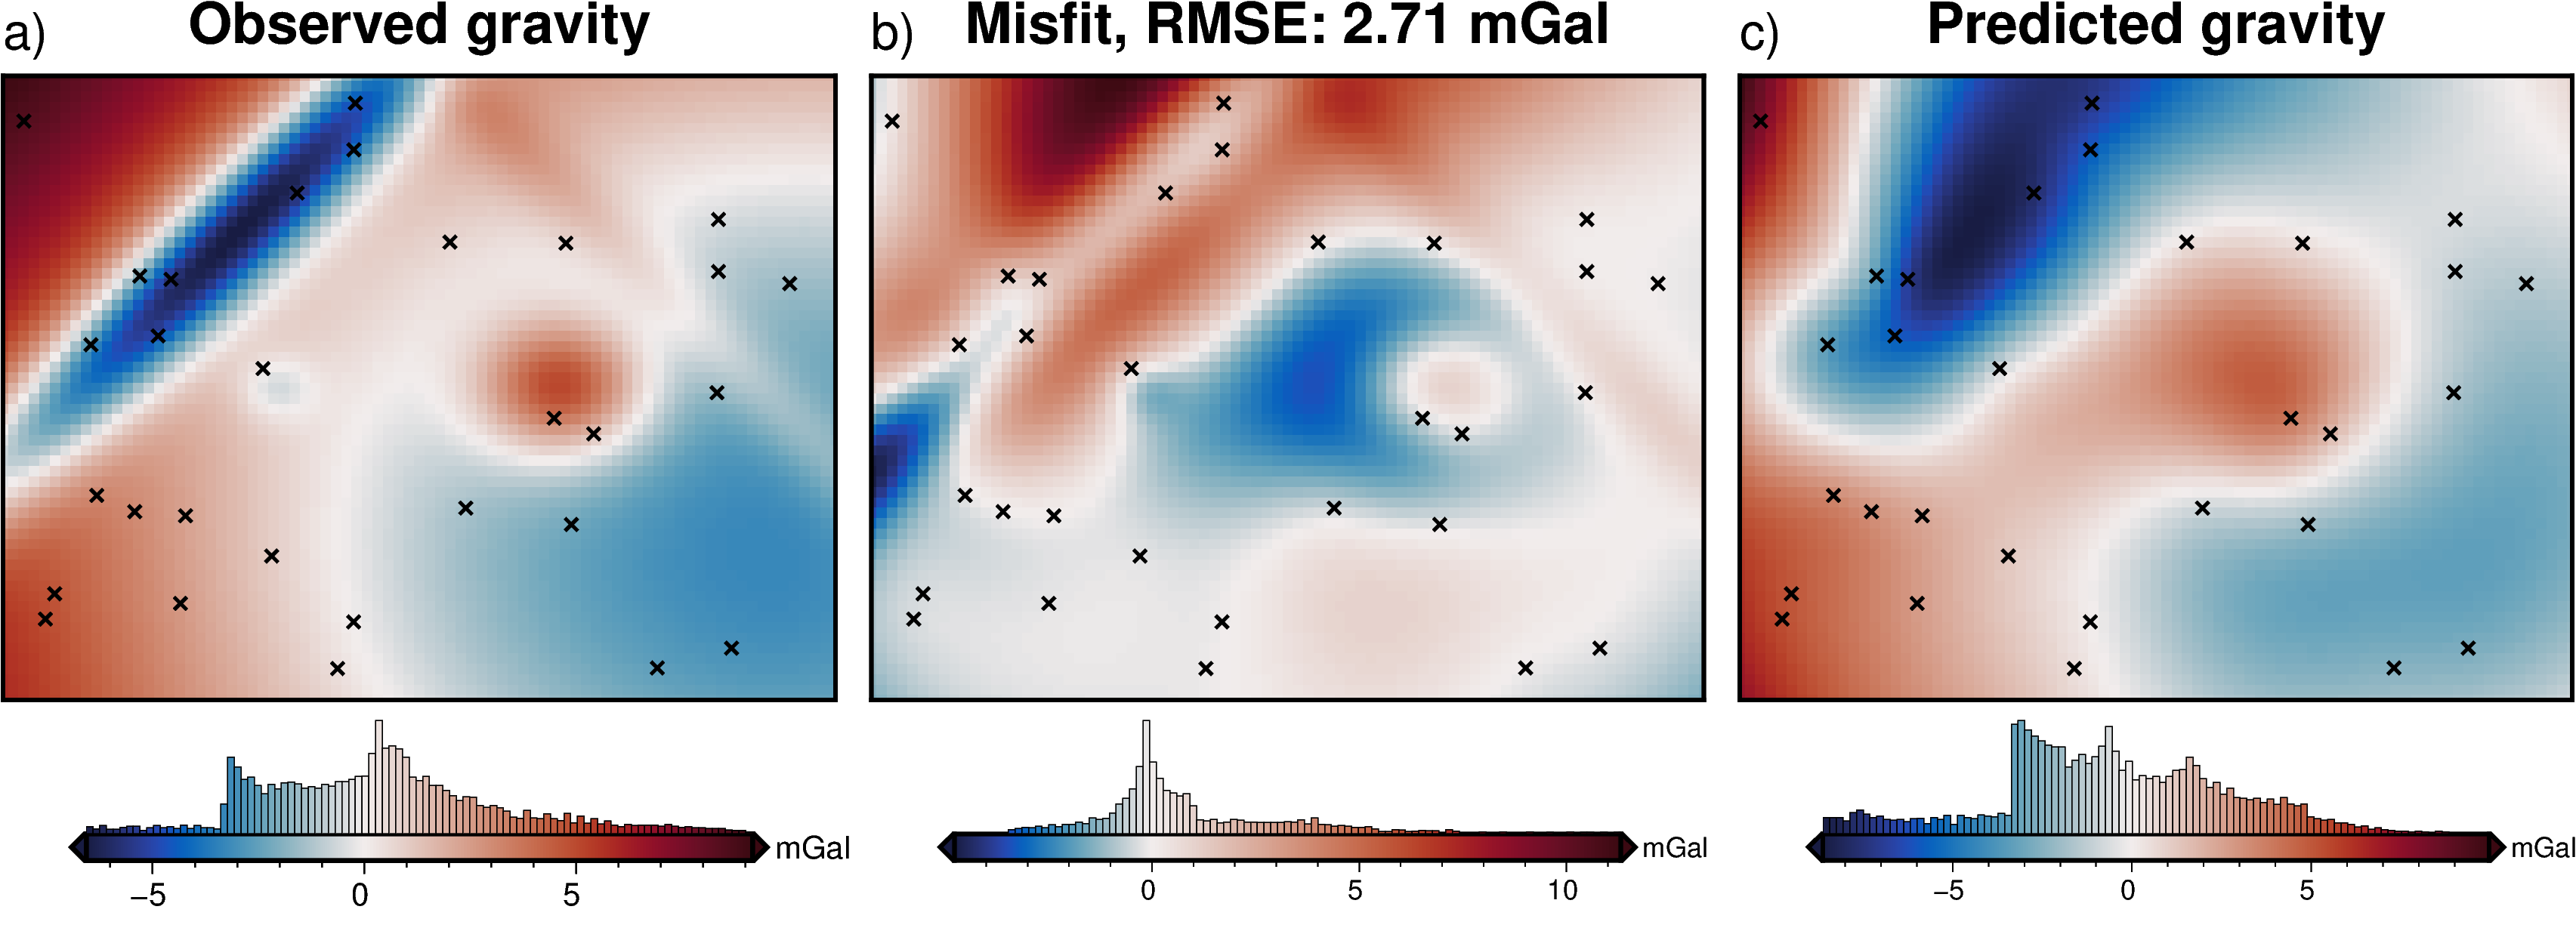
\includegraphics[width=0.95\textwidth]{chp3/chp3_simple_misfit}
    \caption[Simple synthetic gravity anomalies]{\textbf{a)} Synthetic gravity data generated from the true bathymetry, \textbf{b)} the residual anomaly, defined as the difference between a and c, and \textbf{c)} the predicted gravity from the starting bathymetry (Figure \ref{fig:chp3_simple_starting_model}c).}
    \label{fig:chp3_simple_misfit}
\end{figure}

\subsubsection{Cross validation} \label{chp3:simple_model_CV}
To find the optimal value for the regularization damping parameter, the cross-validation method of \citet{uiedafast2017} is used (Section \ref{chp3:regularization}). The full set of observed data with a 500~m spacing ($N$~=~19481), was separated into the training ($N$~=~4941) and testing set ($N$~=~14540). With the grid configuration from Figure \ref{fig:chp3_CV_grid_spacing}, the resulting training data was on a regular 1~km grid, which matches the grid of the bathymetry. This training data set was used as the input to 10 inversions. Each inversion used a different damping value between 10\textsuperscript{-4} and 10\textsuperscript{-1}. The resulting inverted bathymetry of each inversion was then forward-modelled on the observation points of the testing data set (not used in the inversion). The RMS difference between the forward-modelled gravity value and the initial residual misfit values was calculated, giving the cross-validation score (Figure \ref{fig:chp3_simple_CV_and_profile}a). Of the 10 inverted bathymetry models, the model with the lowest score is retained.

\begin{figure}[!ht]
    \centering
    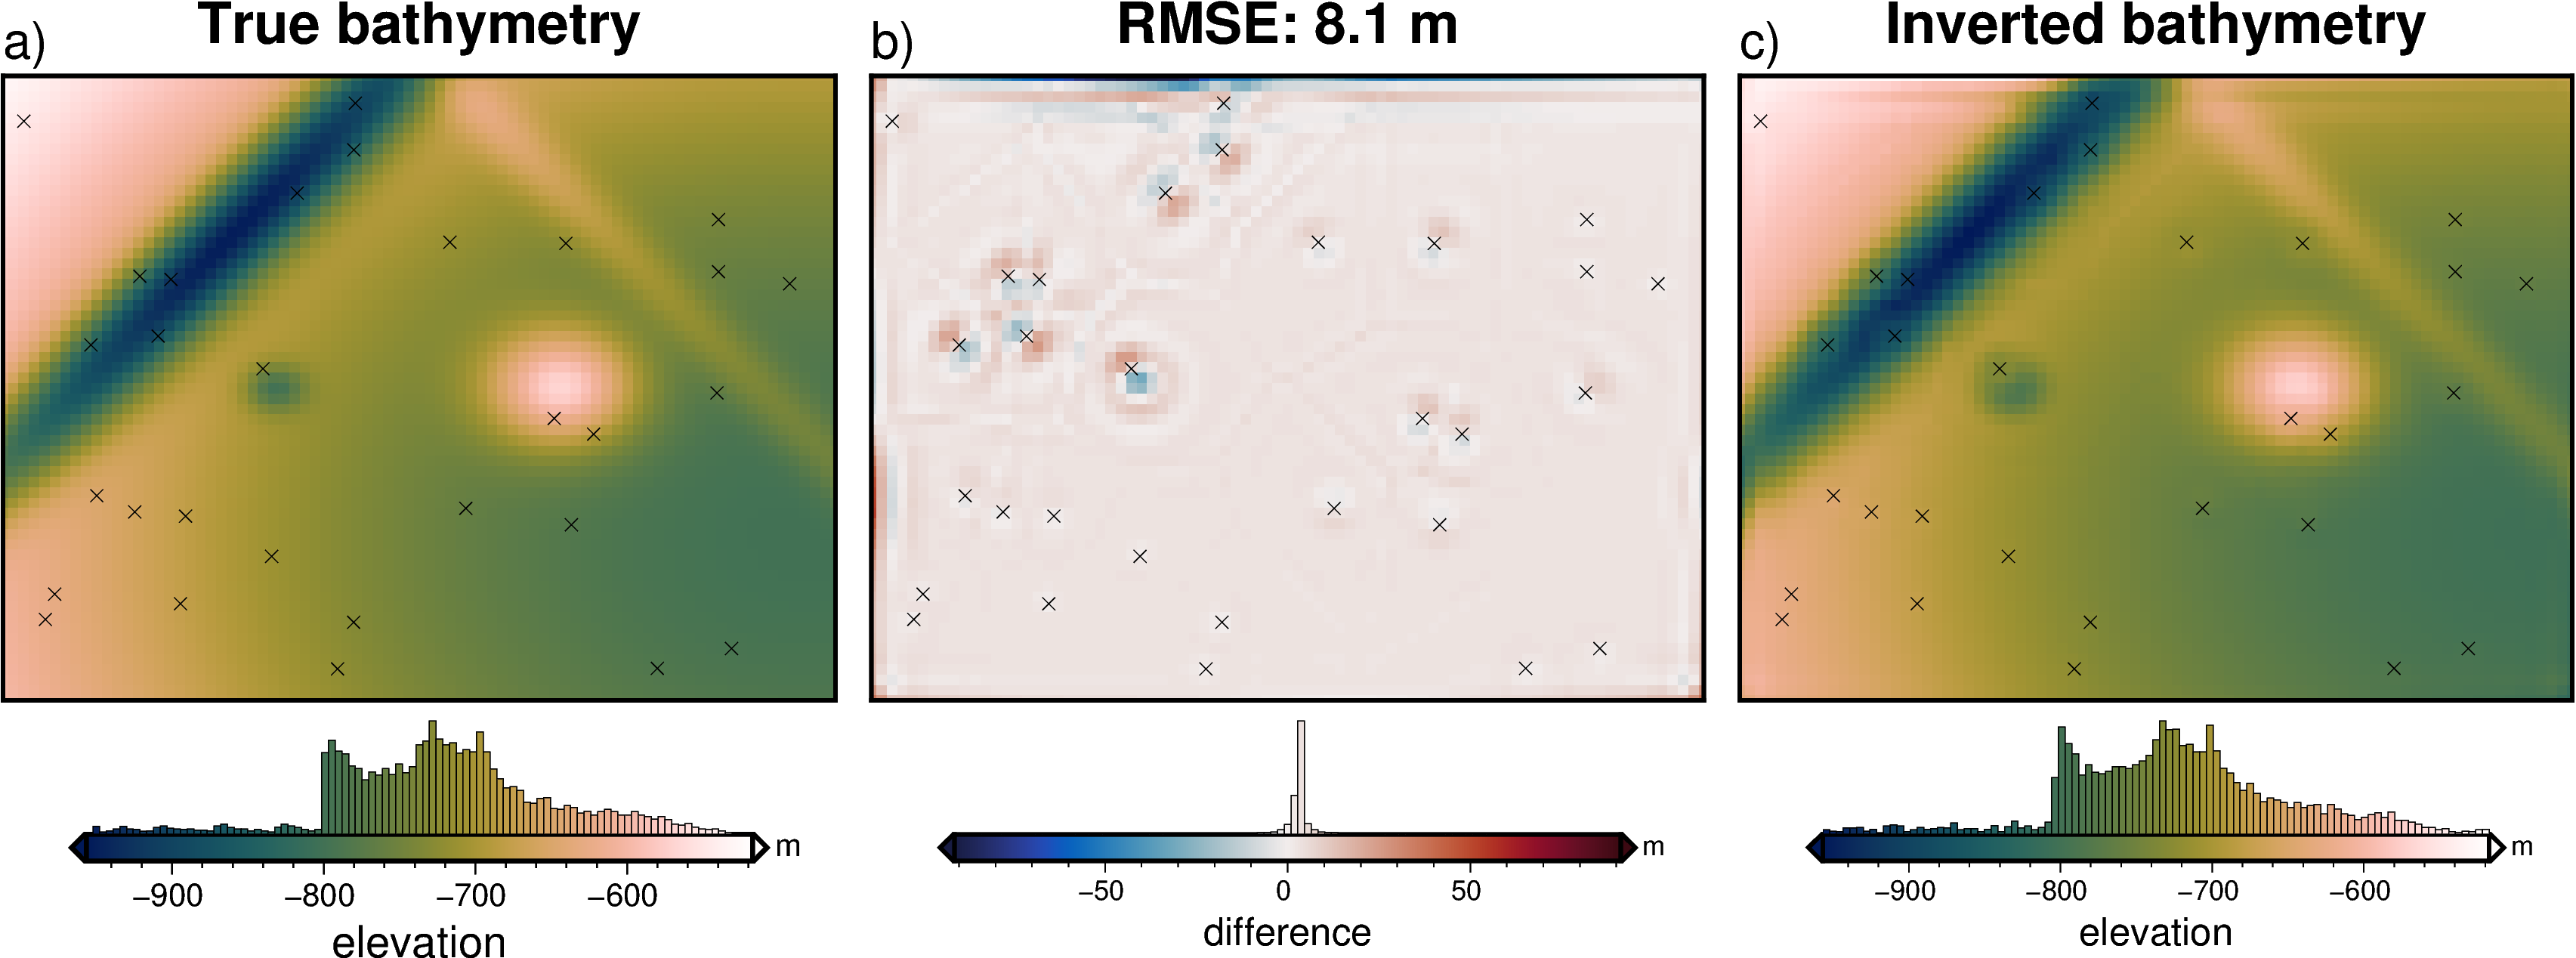
\includegraphics[width=.95\textwidth]{figures/chp3/chp3_simple_results.png}
    \caption[Annulus approximation inversion results]{Inverted results with optimized parameters, using the annulus approximation method of calculating the Jacobian matrix. \textbf{a)} True bathymetry, \textbf{b)} difference between a and c, and \textbf{c)} final inverted bathymetry. Black crosses are constraint points. The RMS difference with the true bathymetry at these constraints is 1 m}
    \label{fig:chp3_simple_results}
\end{figure}

This model is shown in Figure \ref{fig:chp3_simple_results}c, and resulted from a damping value of 10\textsuperscript{-2}. This inverted bathymetry has an RMS difference with the true bathymetry of 8~m and an RMS difference at the constraint points of 1~m. Figure \ref{fig:chp3_simple_CV_and_profile}b shows a profile across the model. The overlap of the true (red) and inverted (blue) bathymetry in the first panel shows the effectiveness of the inversion at recovering the true bathymetry. The lower panel shows the inversion's ability to minimize the misfit between the observed gravity (red) and the forward response of the inverted bathymetry (blue). The inversion was able to recover all the features of the true bathymetry, with only minor errors along the edges of the domain, and adjacent to constraint points. For this simple model, the inversion converged in 37 iterations, with a total computation time of 30~seconds and a final RMS residual misfit of 0.022~mGal. It terminated due to the $\ell^2$-norm decreasing between the set threshold of 0.15 (0.0225~mGal).

\begin{figure}[!ht]
  \centering
    \begin{subfigure}[t]{.40\textwidth}
        \centering
        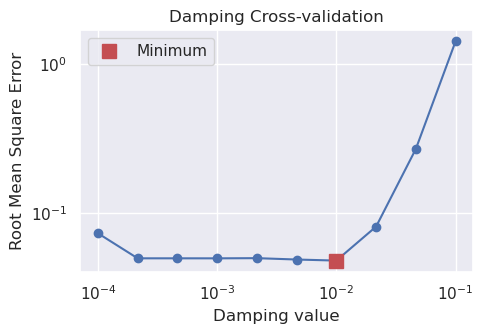
\includegraphics[width=\textwidth]{figures/chp3/chp3_simple_CV.png}
        \caption{}
    \end{subfigure}
    \begin{subfigure}[t]{.58\textwidth}
        \centering
        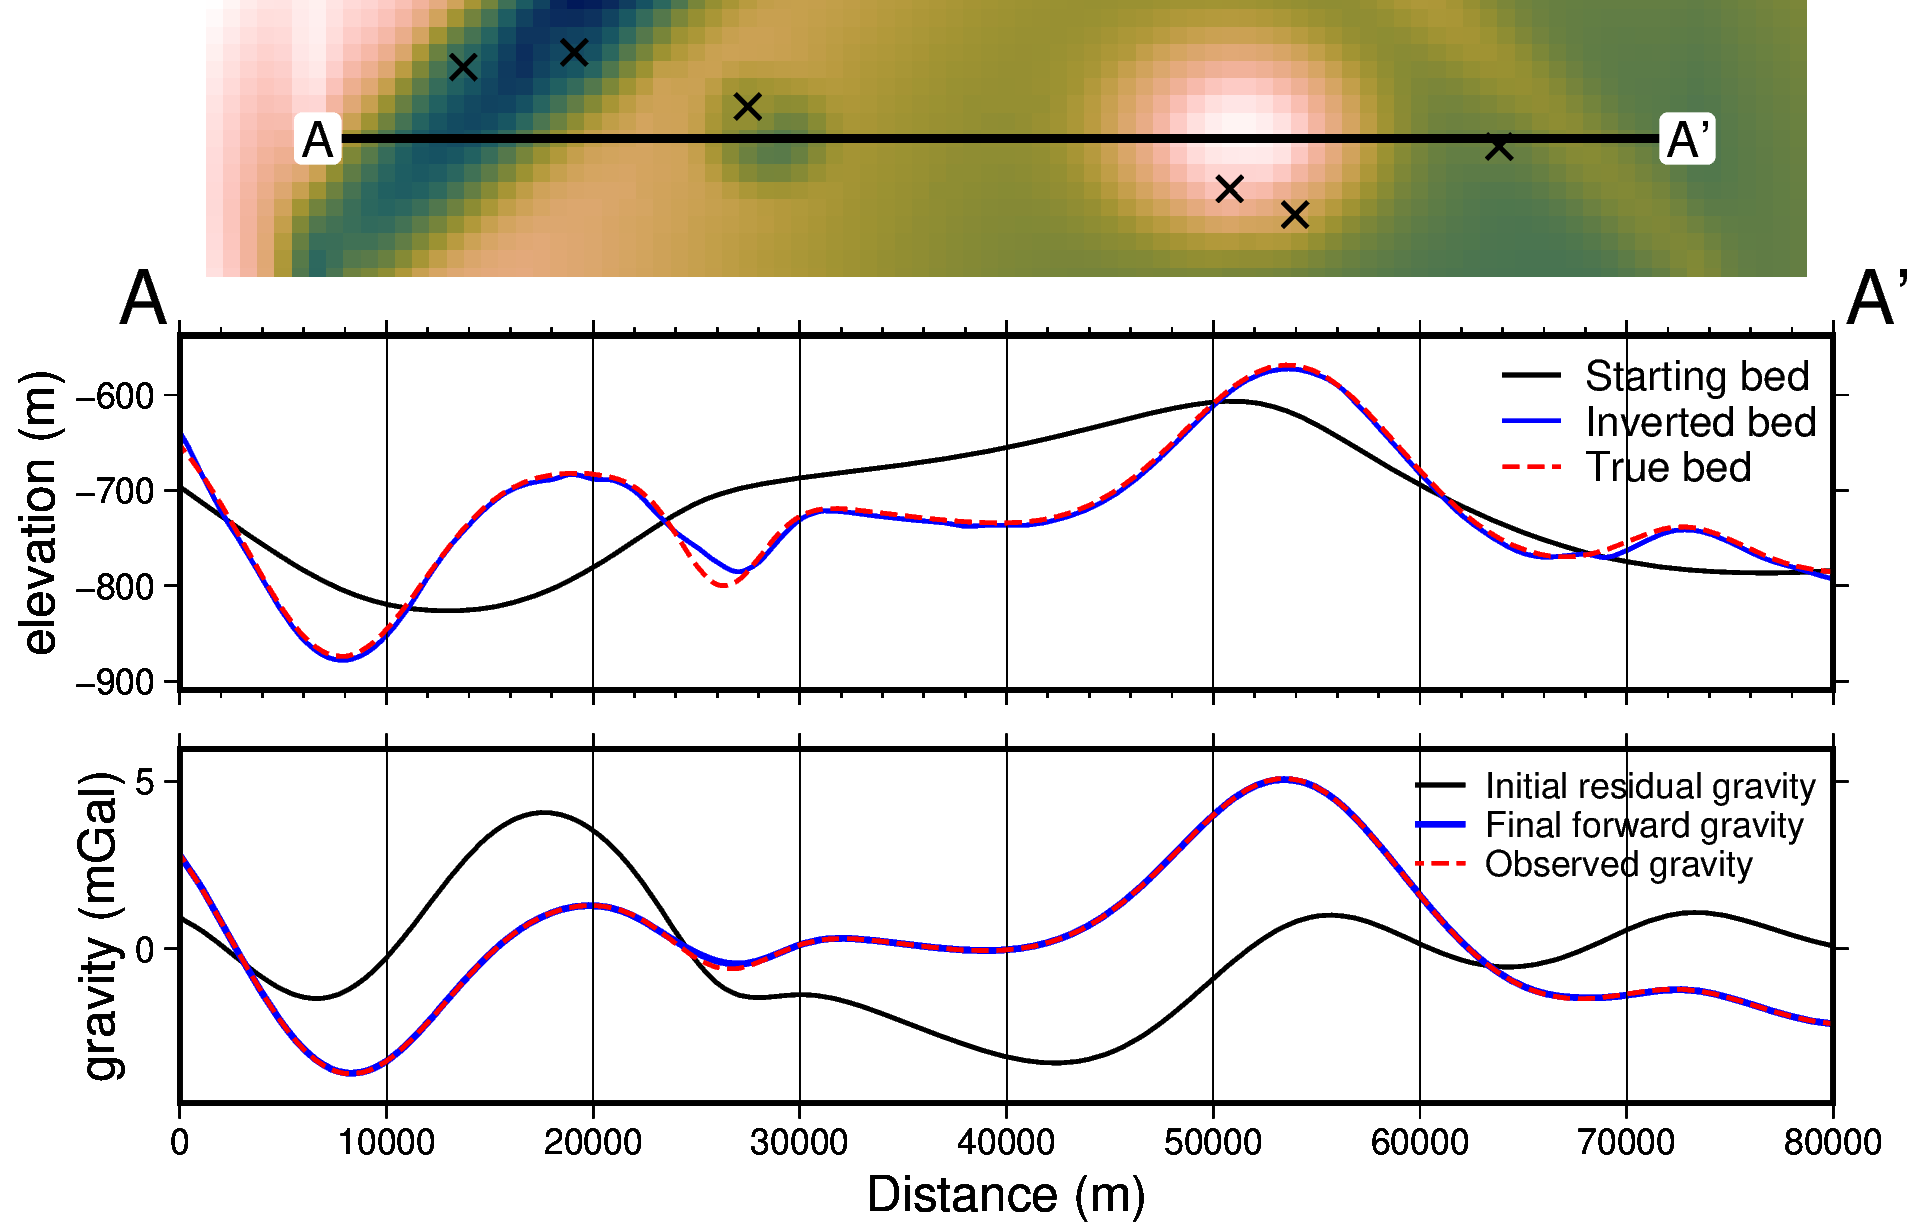
\includegraphics[width=\textwidth]{figures/chp3/chp3_simple_profile.png}
        \caption{}
    \end{subfigure}
  \caption[Annulus approximation inversion cross-validation and profile]{Cross-validation and profiles for the simple synthetic inversion. \textbf{a)} Cross-validation curve showing the optimal damping parameter (red square). Both axes are on a logarithmic scale. \textbf{b)} 2D profile of the inversion results. The top panel shows profile location and constraint points (black crosses). The middle panel contains topographic profiles of the starting, inverted, and true bathymetries. The bottom panel contains gravity anomaly profiles.}
    \label{fig:chp3_simple_CV_and_profile}
\end{figure}

\subsubsection{Comparing vertical derivative methods} \label{chp3_annulus_vs_prisms}
Section \ref{chp3:jacobian_methods} presented two methods for calculating the vertical derivative of gravity of a prism. This vertical derivative is used to create the Jacobian matrix (Equation \ref{eq:matrix_eq}) and needs to be calculated at each iteration of the inversion. The above cross-validation and inversion were performed using the \textit{annulus approximation} of the vertical derivative. Here, this process is repeated with the \textit{finite differences} method of the vertical derivative. Figure \ref{fig:chp3_simple_prisms_approx_results}) shows the results of this inversion. The optimal damping parameter was 10\textsuperscript{-2}, and the inversion resulted in an RMS difference with the true bathymetry of 9~m, compared to 8~m for the annulus approximation. Figure \ref{fig:chp3_annulus_vs_prisms_convergence} shows the inversion convergence curves for the inversion of the annulus approximation and the finite differences methods. The inversion with the annulus approximation was $\sim$500\% faster to converge than the finite differences method (30~sec vs 169~sec). Because these vertical derivatives need to be recalculated at each iteration, a large portion of the inversion time is spent performing these calculations. This comparison shows the annulus approximation is not only significantly faster, but results in comparable, or slightly more accurate, inversion results. For the remainder of this chapter, only the annulus approximation will be used.

\begin{figure}[!ht]
    \centering
    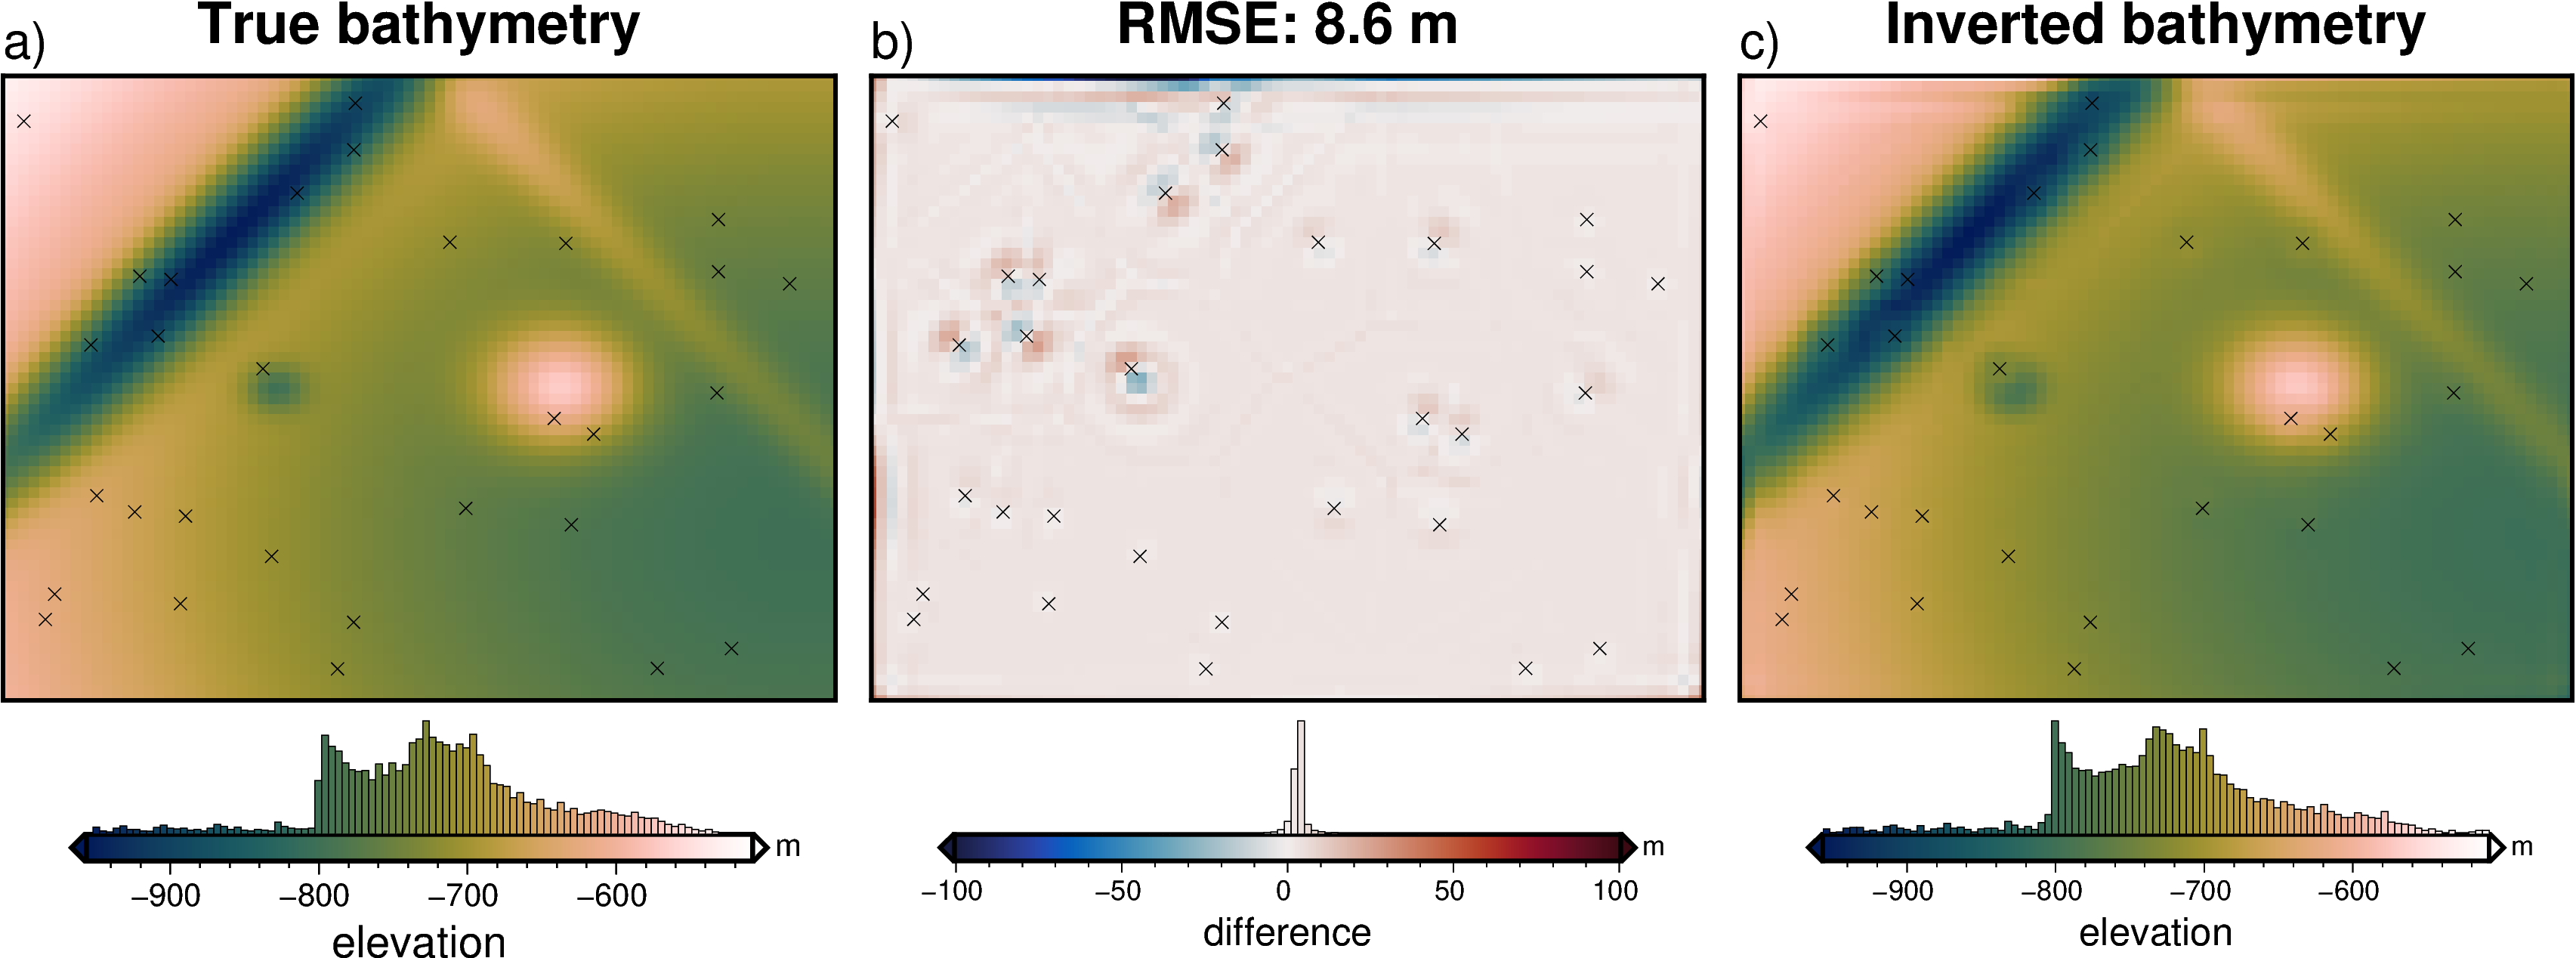
\includegraphics[width=.95\textwidth]{figures/chp3/chp3_simple_prisms_derivative_results.png}
    \caption[Finite differences inversion results]{Inversion results with optimized parameters using the finite differences method. \textbf{a)} True bathymetry, \textbf{b)} difference between a and c, and \textbf{c)} final inverted bathymetry. Black crosses are constraint points. The RMS difference with the true bathymetry at these constraints is 1~m}
    \label{fig:chp3_simple_prisms_approx_results}
\end{figure}

\begin{figure}[!ht]
  \centering
    \begin{subfigure}[t]{.48\textwidth}
        \centering
        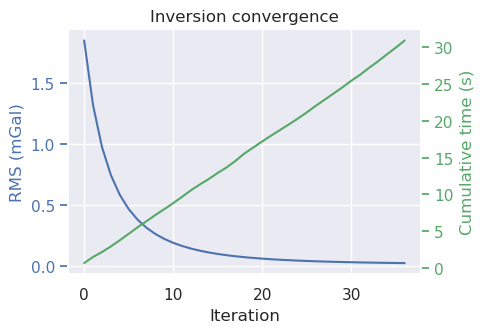
\includegraphics[width=\textwidth]{figures/chp3/chp3_simple_convergence.png}
        \caption{}
    \end{subfigure}
    \begin{subfigure}[t]{.48\textwidth}
        \centering
        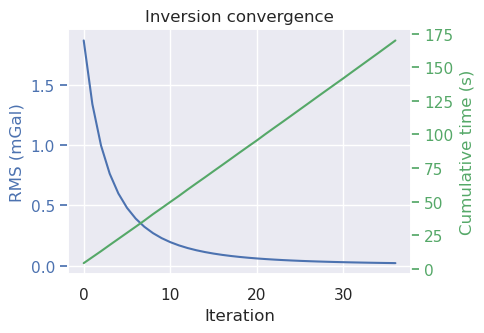
\includegraphics[width=\textwidth]{figures/chp3/chp3_simple_prisms_derivative_convergence.png}
        \caption{}
    \end{subfigure}
  \caption[Finite differences and annulus approximation convergence curves]{Inversion convergence curves for the two methods of creating the Jacobian matrix. Blue line (left y-axis) shows the RMS of the residual misfit at each iteration of the inversion. Green line (right y-axis) shows the cumulative time to complete the inversion. \textbf{a)} Results for the annulus approximation method of finding the vertical derivative. \textbf{b)} Results for the finite differences method.}
    \label{fig:chp3_annulus_vs_prisms_convergence}
\end{figure}

\subsubsection{Added noise}
To test the effect of noise in the gravity data, which is inevitable in data collection, especially so in airborne surveying, the observed gravity was contaminated with noise. The noise has a Gaussian distribution with a mean of 0~mGal and a standard deviation of 2\% of the max absolute value of the data ($\sim$ .16~mGal). Similarly, \citet{rashidifardconstraining2021} used 5\% noise in their synthetic gravity inversion while \citet{uiedafast2017} use 5~mGal of noise, which for their synthetic application equated to $\sim$~1\% of the max absolute value. Using this noise-corrupted gravity data, the same damping parameter cross-validation was run as previously (Figure \ref{fig:chp3_simple_noise_CV_and_profile}a), and the lowest score was achieved with a damping value of 10\textsuperscript{-2}. Figure \ref{fig:chp3_simple_noise_results} shows the inversion results of this noise-contaminated model. 
The inversion converged in 18 iterations, with a total computation time of 13 seconds and a final RMS residual misfit of 0.16~mGal. It terminated after the $\ell^2$-norm became lower than the set tolerance of 0.4 (0.16~mGal). This tolerance was set to match the known level of noise. The inverted bathymetry had an RMS difference of 12~m with the true bathymetry and an RMS difference of $<$~1~m at the constraint points. Figure \ref{fig:chp3_simple_noise_CV_and_profile}b shows the inversion is still able to reproduce the observed gravity (lower panel), but a component of the noise was introduced into the final bathymetry (upper panel). All major features of the true bathymetry are recovered, albeit not as accurately as the no-noise model (Figure \ref{fig:chp3_simple_results}).

\begin{figure}[!ht]
    \centering
    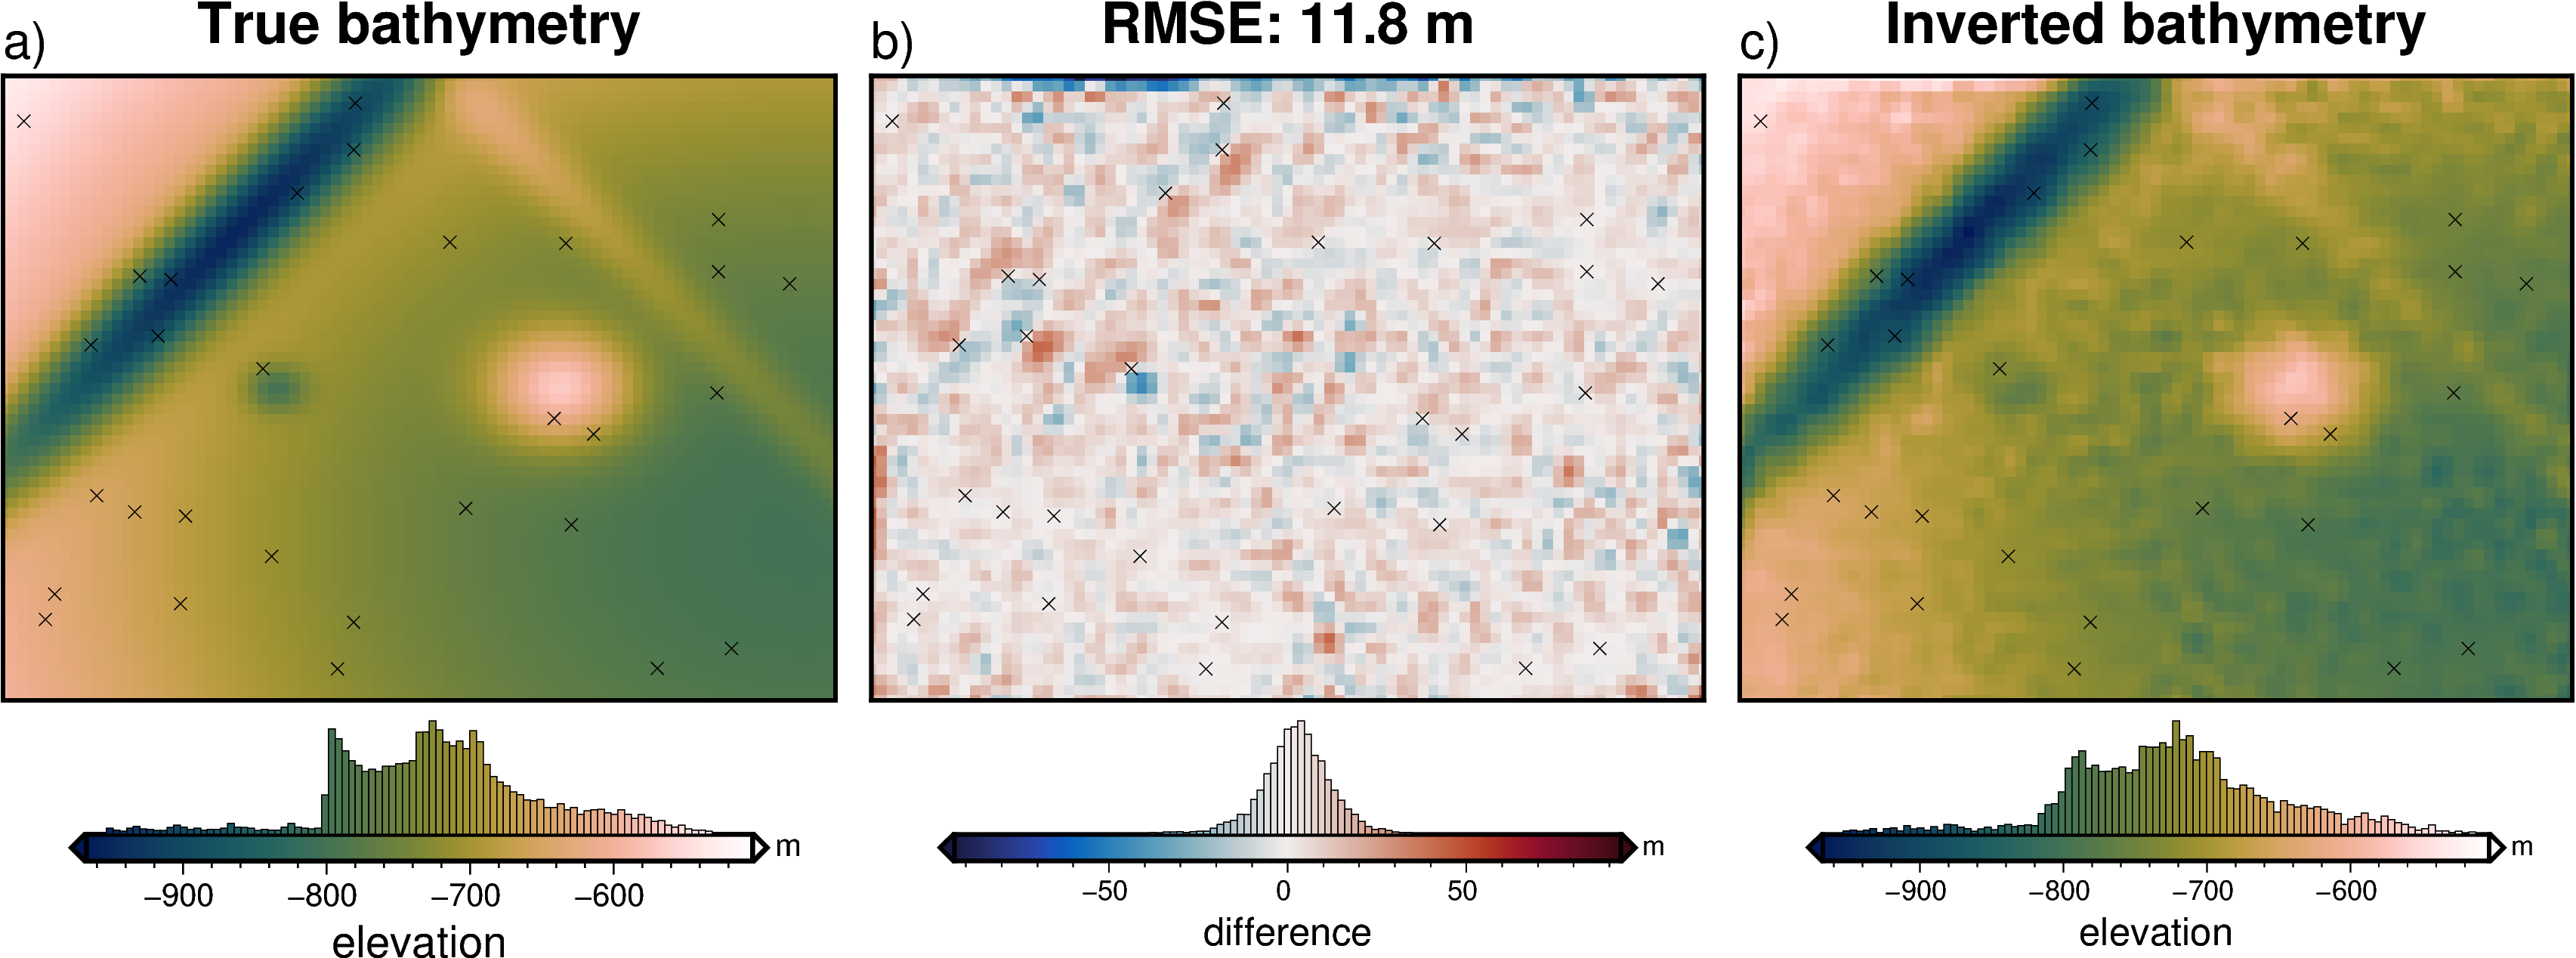
\includegraphics[width=0.95\textwidth]{chp3/chp3_simple_noise_results}
    \caption[Synthetic inversion with noise]{Simple synthetic model inversion results with 2\% added noise (0.16~mGal). \textbf{a)} True bathymetry, \textbf{b)} difference between a and c, \textbf{c)} final inverted bathymetry. Black crosses are constraint points. The RMS difference with the true bathymetry at these constraints is $<$~1~m.}
    \label{fig:chp3_simple_noise_results}
\end{figure}

\begin{figure}[!ht]
  \centering
    \begin{subfigure}[t]{.40\textwidth}
        \centering
        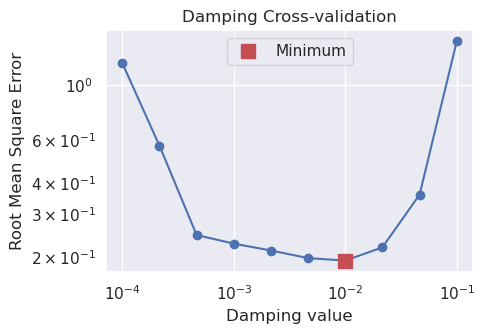
\includegraphics[width=\textwidth]{figures/chp3/chp3_simple_noise_CV.png}
        \caption{}
    \end{subfigure}
    \begin{subfigure}[t]{.58\textwidth}
        \centering
        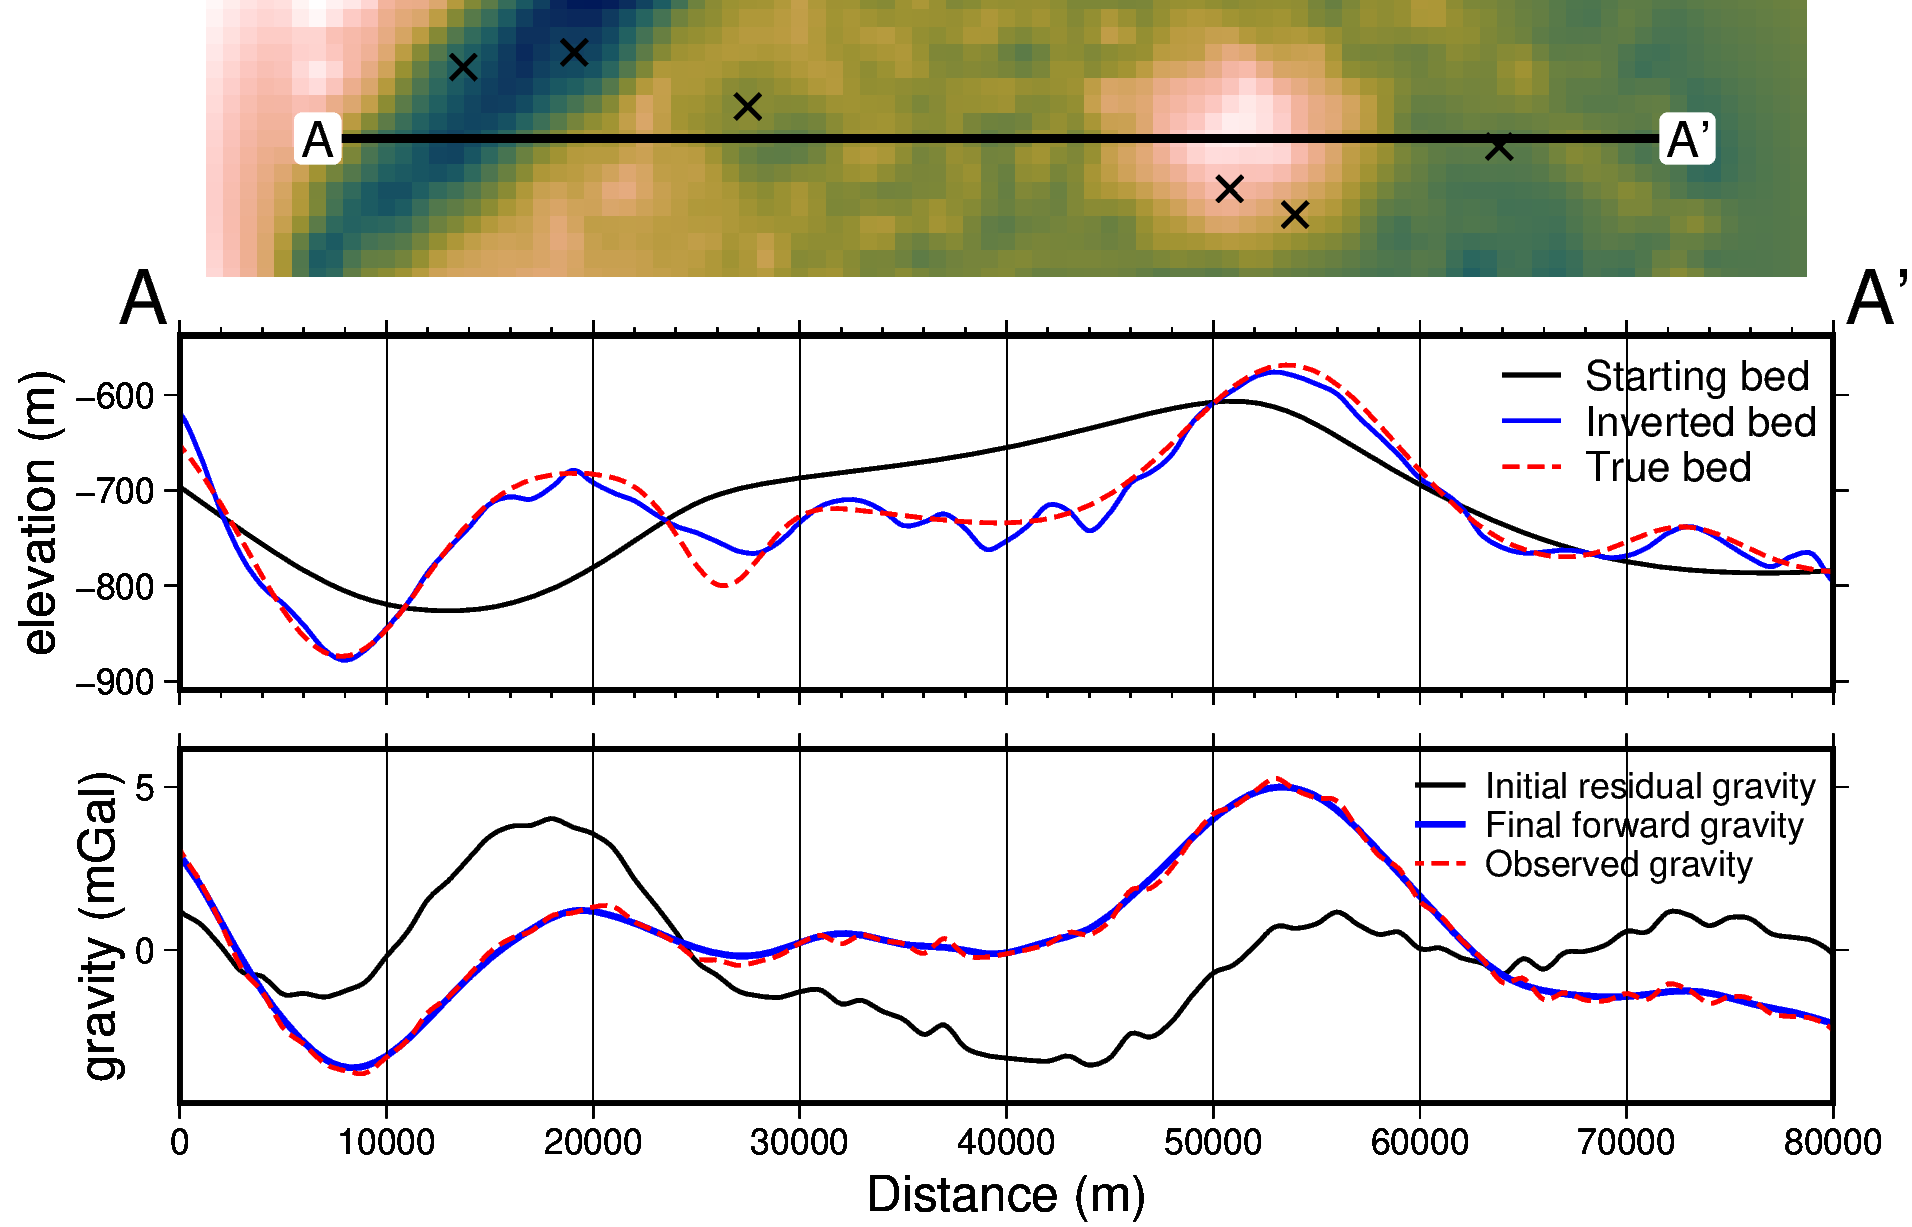
\includegraphics[width=\textwidth]{figures/chp3/chp3_simple_noise_profile.png}
        \caption{}
    \end{subfigure}
  \caption[Synthetic inversion with noise, CV and profile]{Cross-validation and profiles for the inversion with noise. \textbf{a)} Cross-validation curve showing the optimal damping parameter (red square). \textbf{b)} 2D profile of the inversion results. The top panel shows profile location and constraint points (black crosses). The middle panel contains topographic profiles of the starting, inverted, and true bathymetries. The bottom panel contains gravity anomaly profiles.}
    \label{fig:chp3_simple_noise_CV_and_profile}
\end{figure}

\subsubsection{Down-sampled data} \label{chp3:eq source resampled}
The previous two models used observed gravity data collected on a grid of observation points at the same grid spacing as the prism layer (1~km). This represents a very dense gravity survey. Gravity surveys are often relatively sparse compared to the resolution of the surface they are attempting to recover in an inversion. This section tests the effect of changing the resolution of the gravity data, to simulate a coarser gravity survey. Simply sampling the gravity data at a coarser resolution leads to a checker-boarding effect, where the inversion alters prisms nearby the gravity observations, but not prisms further away. 
For this reason, it is recommended here to re-grid the observed gravity data at a similar grid spacing to the prism layer. This can be accomplished with standard gridding techniques, such as minimum curvature or bi-harmonic splines (see section \ref{chp3_gridding_comparison}). However, these techniques aren't well suited for potential field data since they don't account for the variation in observation heights \citep{solergradientboosted2021}. An alternative method of interpolating the gravity data onto a finer resolution grid is the equivalent sources technique \citep{dampneyequivalent1969}\footnote{The equivalent sources technique is also used in this study as a means of regional separation (see section \ref{chp3_regional_seperation}, this is a similar application but for different purposes.}. \\

\begin{figure}[!ht]
\renewcommand\thesubfigure{\arabic{subfigure}}
  \centering
    \begin{subfigure}[t]{.95\textwidth}
        \centering
        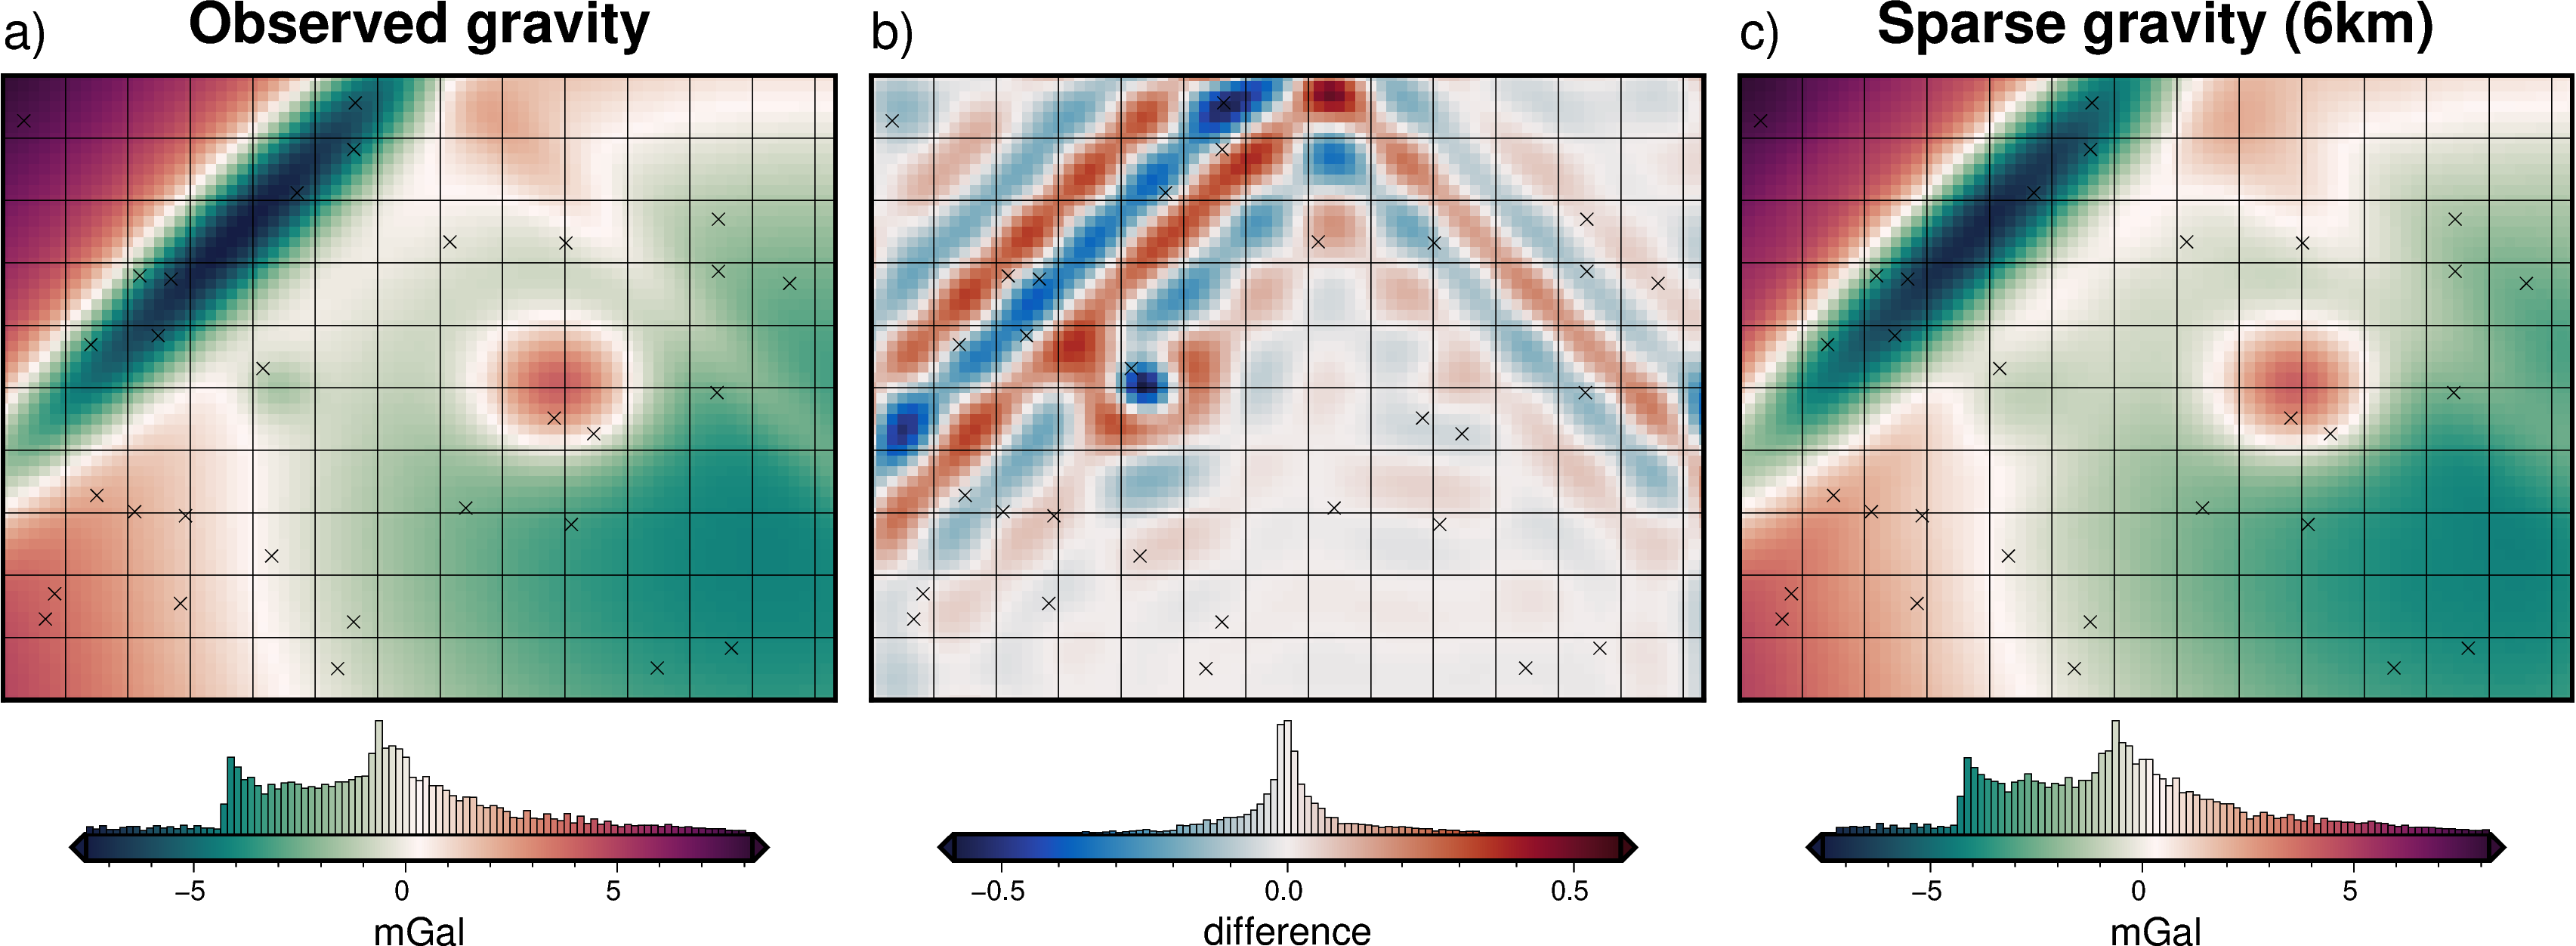
\includegraphics[width=\textwidth]{figures/chp3/chp3_simple_sampled_gravity_eq_sources.png}
        \caption{Equivalent sources re-gridding}
    \end{subfigure}
    \begin{subfigure}[t]{.95\textwidth}
        \centering
        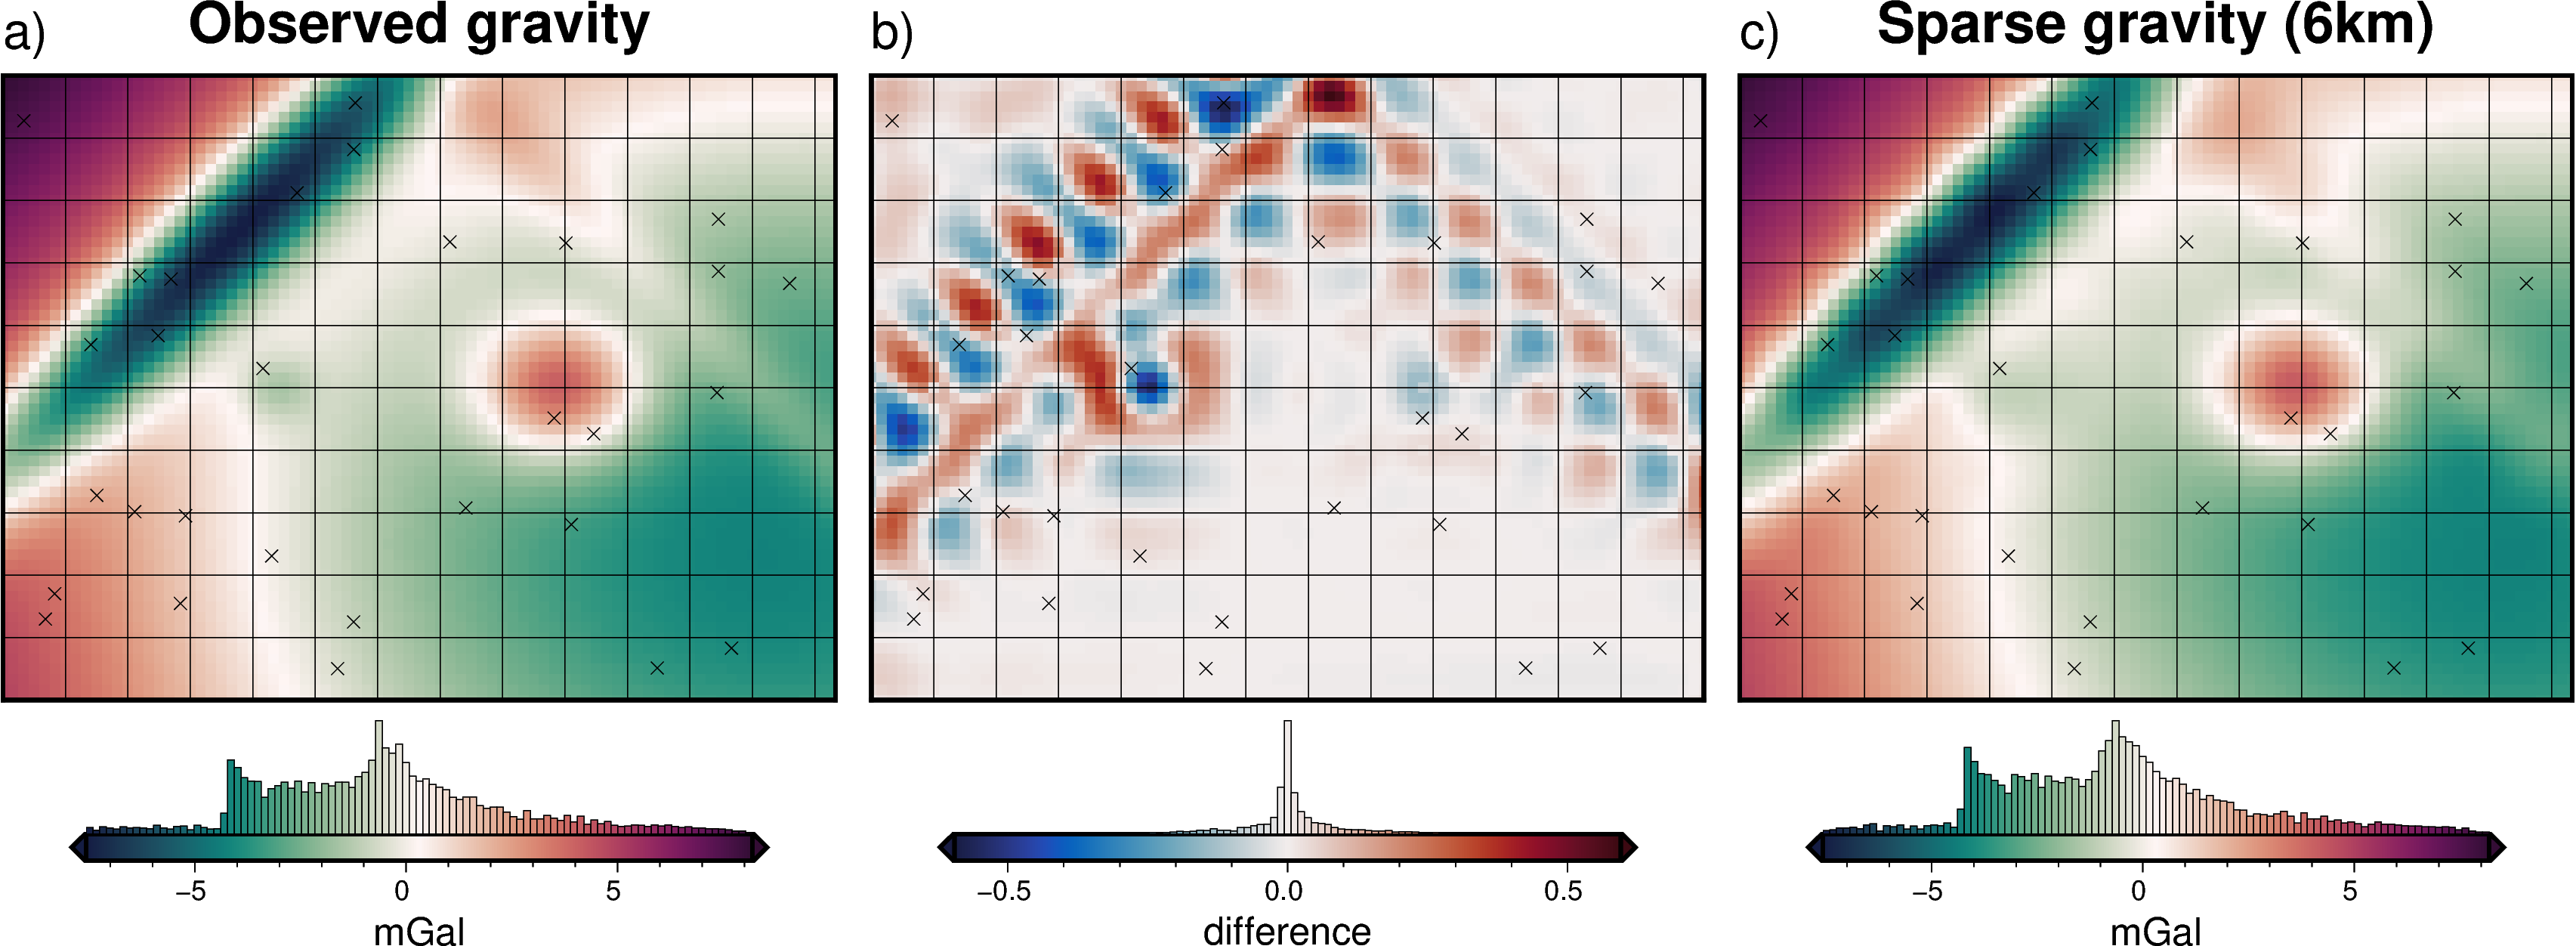
\includegraphics[width=\textwidth]{figures/chp3/chp3_simple_sampled_gravity_regular_gridding.png}
        \caption{Bi-harmonic spline re-gridding}
    \end{subfigure}
  \caption[Creating a low-resolution observed gravity survey]{Creating a low-resolution observed gravity survey. \textbf{Top panel} shows results using the equivalent source technique of gridding gravity data. \textbf{Bottom panel} shows simple gridding using a bi-harmonic spline. \textbf{a)} Original observed data on a 1~km grid, \textbf{b)} gravity signal lost due to sampling and re-gridding, \textbf{c)} the low-resolution observed gravity (6~km spacing) re-gridded at 1~km with either equivalent sources (top) or a regular gridding algorithm (bottom). Black crosses show constraint points and black lines show 6~km grid.}
    \label{fig:chp3_simple_eq_sources_regridding}
\end{figure}

Here, the original gravity data, on a 1~km grid, is sampled at a 6~km spaced grid to represent a low-resolution survey with observations every 6~km. A series of point sources are created at depth, and their densities are altered to best reproduce the observed gravity data. Once this process of fitting the source parameters to the data is accomplished, the gravity field can be predicted anywhere. For this application, the equivalent sources are predicted onto an even 1~km grid, to match the spacing of the bathymetry. Figure \ref{fig:chp3_simple_eq_sources_regridding} shows the results of this process (top panel) and the results using simple gridding without equivalent sources (bottom panel). \textit{Subplot a} shows the original observed gravity data (just training points) on a 1~km grid. This grid is sampled onto a 6~km grid (black grid lines) and re-gridded at 1~km (\textit{subplot c}). \textit{Subplot b} shows the difference, which represents the lost data resulting from the sparse survey. Typically the equivalent sources gridding technique is most beneficial to account for variations in observation heights. Here, even with constant elevations, there are noticeable differences between equivalent source gridding and simple gridding with bi-harmonic splines. \\

The equivalent-source resampled grid is used, with no added noise, in the same inversion procedure as the previous sections. The cross-validation (Figure \ref{fig:chp3_simple_sampled_CV_and_profile}a) resulted in an optimal damping value of 10\textsuperscript{-2}. The inverted bathymetry with this damping value is shown in Figure \ref{fig:chp3_simple_sampled_results}. The inversion was completed in 29~seconds and 38~iterations with a final RMS residual misfit of 0.019~mGal. The inversion was terminated due to the $\ell^2$-norm decreasing below the set threshold of 0.15~mGal\textsuperscript{1/2}. The inverted bathymetry had an RMS difference of 11 m with the true bathymetry and an RMS difference of 1~m at the constraint points. While the overall difference from the true bathymetry is low, this inversion failed to fully recover the small circular depression. Figure \ref{fig:chp3_simple_eq_sources_regridding} shows that the nearest observation point (intersection of gridlines) was on either side of this anomaly, and thus the sparse gravity survey used here failed to image the true magnitude of the feature. Figure \ref{fig:chp3_simple_sampled_results}b shows the absence of this feature in the inverted bathymetry. 

\begin{figure}[!ht]
    \centering
    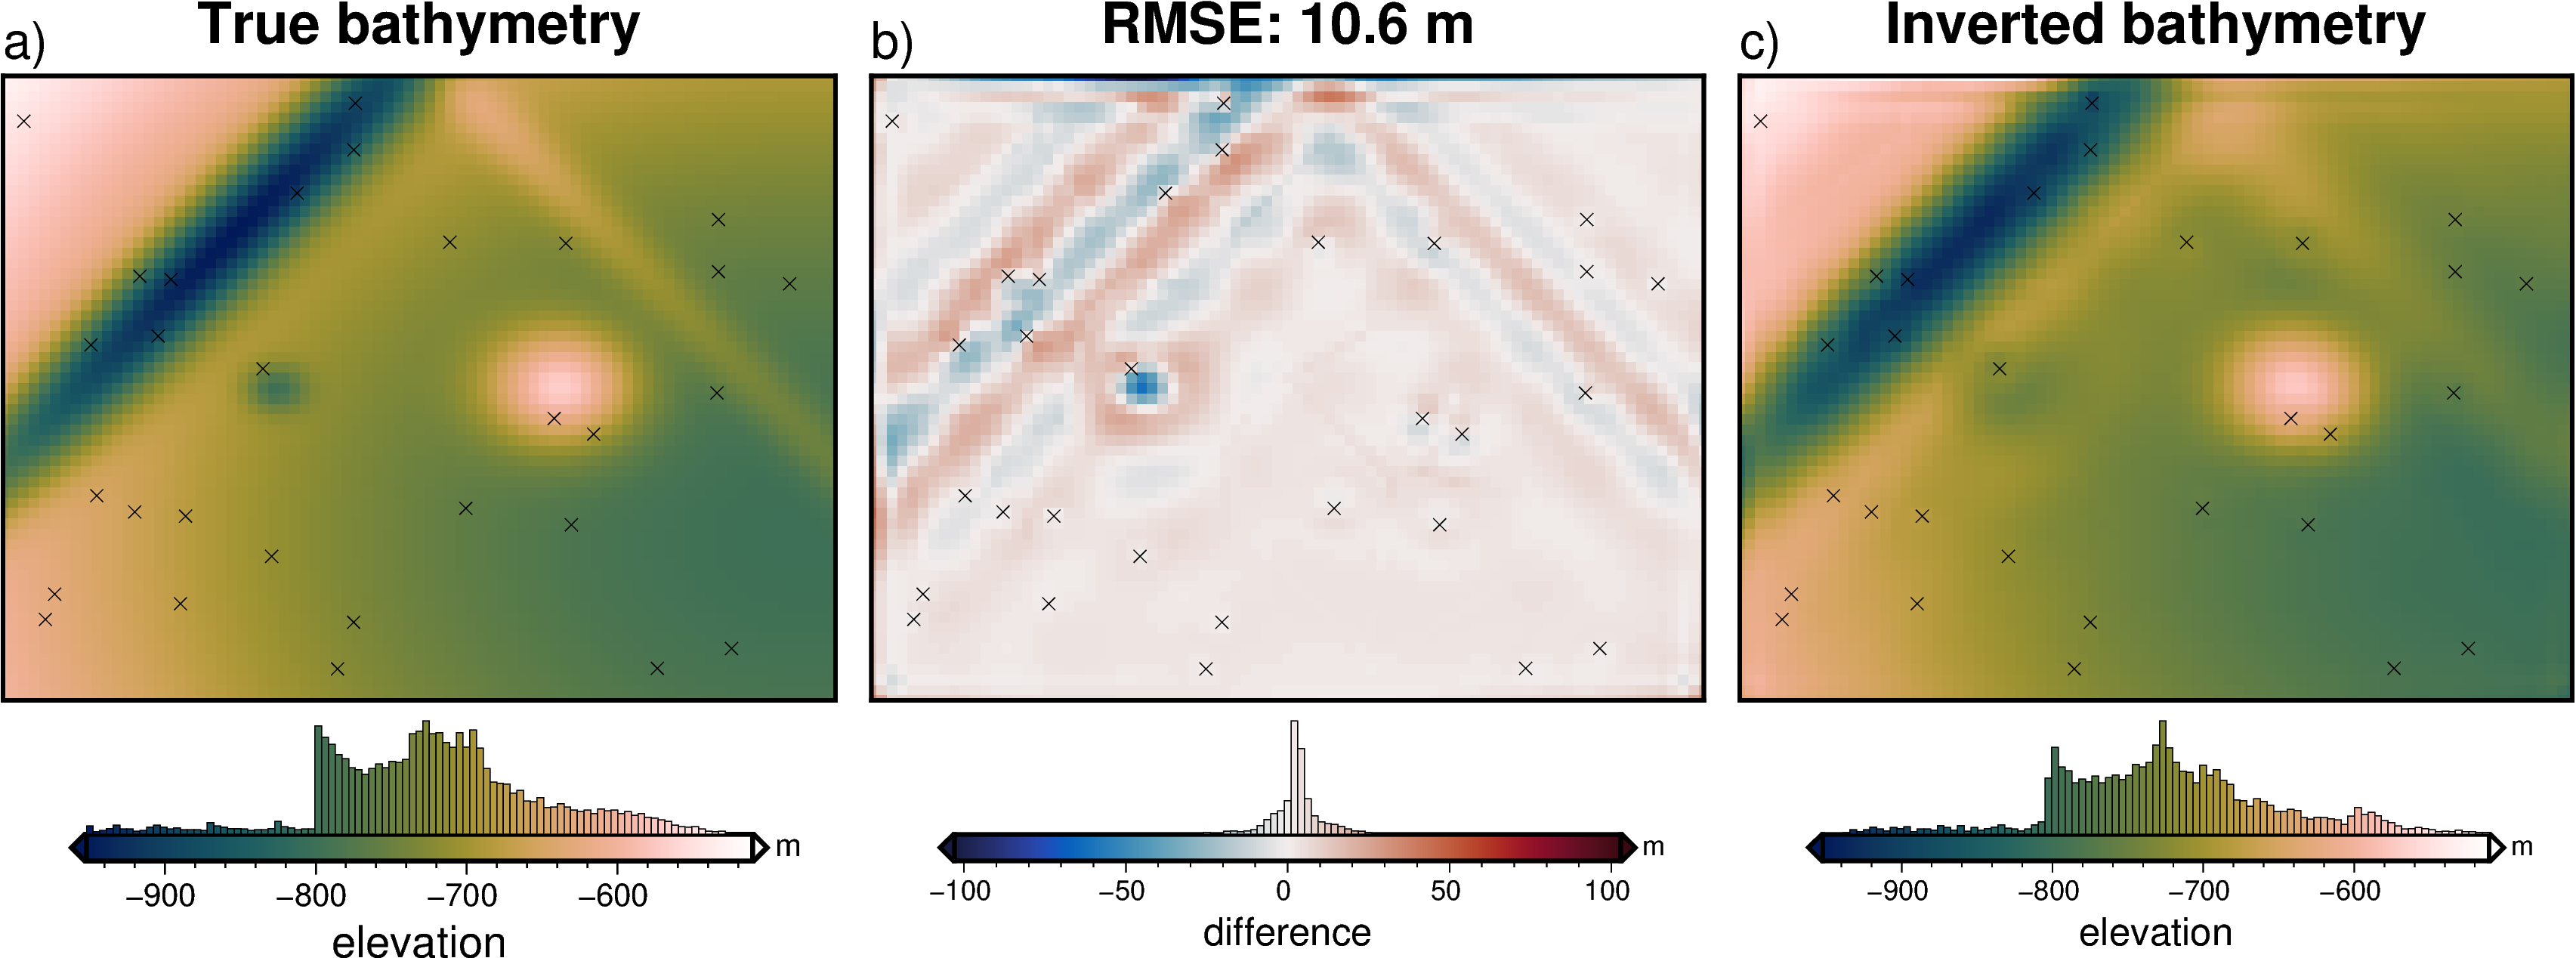
\includegraphics[width=0.95\textwidth]{chp3/chp3_simple_sampled_results}
    \caption[Synthetic inversion with sampled gravity]{Simple synthetic model inversion results with input data resampled at 6x the bathymetry grid spacing (6~km). \textbf{a)} True bathymetry, \textbf{b)} difference between a and c, and \textbf{c)} final inverted bathymetry. Black crosses show constraint points. The RMS difference with the true bathymetry at these constraints is 1~m.}
    \label{fig:chp3_simple_sampled_results}
\end{figure}

\begin{figure}[!ht]
  \centering
    \begin{subfigure}[t]{.40\textwidth}
        \centering
        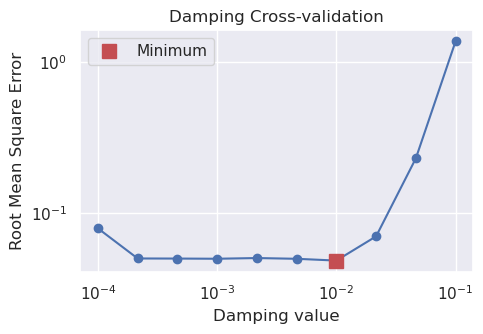
\includegraphics[width=\textwidth]{figures/chp3/chp3_simple_sampled_CV.png}
        \caption{}
    \end{subfigure}
    \begin{subfigure}[t]{.58\textwidth}
        \centering
        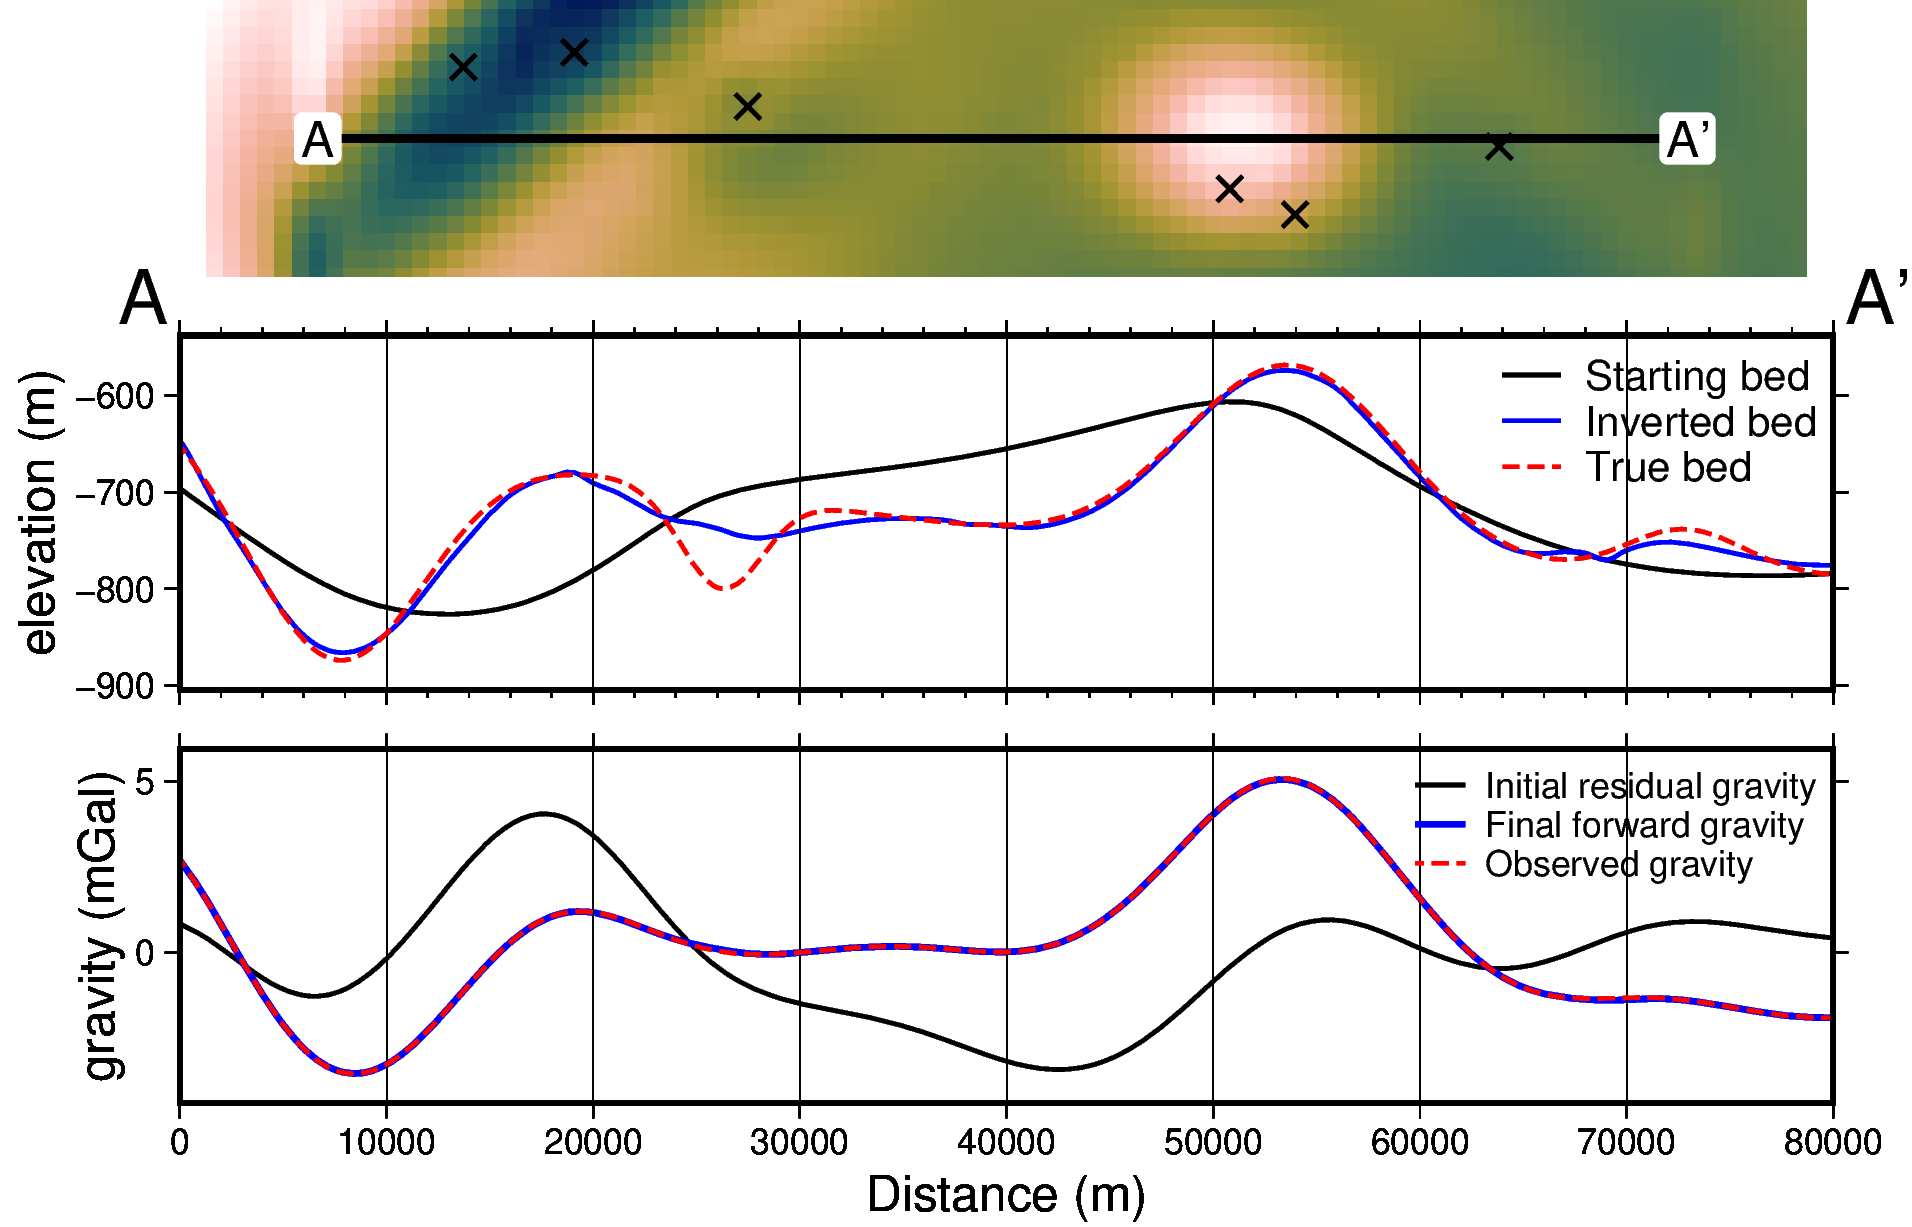
\includegraphics[width=\textwidth]{figures/chp3/chp3_simple_sampled_profile.png}
        \caption{}
    \end{subfigure}
  \caption[Synthetic inversion with sampled gravity, CV and profile]{Cross-validation and profiles for the 6~km resampled inversion. \textbf{a)} Cross-validation curve showing the optimal damping parameter. \textbf{b)} 2D profile of the inversion results. The top panel shows profile location and constraint points (black crosses). The middle panel contains topographic profiles of the starting, inverted, and true bathymetries. The bottom panel contains gravity anomaly profiles.}
    \label{fig:chp3_simple_sampled_CV_and_profile}
\end{figure}

\subsection{Ensemble of Noise and Sampling values} \label{chp3:simple_ensemble}

\begin{figure}[!ht]
    \centering
    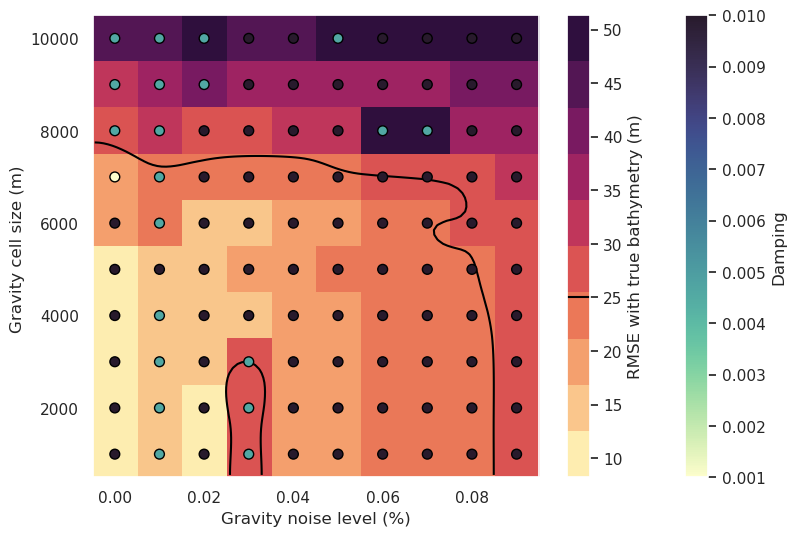
\includegraphics[width=0.9\textwidth]{figures/chp3/chp3_simple_ensemble.png}
    \caption[Gravity data ensemble for synthetic model]{Ensemble of noise levels and gravity spacing for the simple synthetic model. Grid cell colour indicates each inversion's RMS difference with the true bathymetry. The circles' colour indicates the optimal damping value found for each inversion's cross-validation. Black line shows the 25~m RMSE contour, indicative of the amplitude of the smallest amplitude features.}
    \label{fig:chp3_simple_ensemble}
\end{figure}

To test the relative importance of the level of noise and the resolution of the gravity data (i.e. station/flight line spacing), an ensemble of 100 inversions was run, with 10 noise levels between 0 and 9\%, and 10 gravity resolutions between 1 and 10~km. The noise level percentages are of the maximum absolute value of the data, equating to 10 levels between 0 and 0.85~mGal. The differing gravity resolutions were created with the sampling and re-gridding of equivalent sources outlined in the above section. For each set of noise and spacing values, the cross-validation routine was used to find the optimal damping parameters and associated inverted bathymetries. Each of these 100 inversions were then compared to the true bathymetry yielding an RMS difference for each. 

Figure \ref{fig:chp3_simple_ensemble} shows the results of this ensemble of inversion. Each grid cell represents a single inversion, with the level of noise and gravity resolution for the inversion indicated by the x and y axis, respectively. The background colour (warm colours) indicates each inversion's resulting RMS difference with the true bathymetry. Coloured circles show the optimal damping value for each inversion found through cross-validation. This shows a general decrease in the inversion's accuracy with either more noise or lower-resolution gravity data. The smallest bathymetric features which this inversion ideally should recover have amplitudes of tens of meters (small circular depression and narrow ridge). The RMSE here indicates a base-level of error in the inversions, while the error in the vicinity of the short wavelength bathymetry features is likely higher (Figure \ref{fig:chp3_simple_sampled_results}b). Inversions with RMSEs of 10's of meters will likely fail to resolve these small features. For this inversion, an RMSE of 25~m (black contour in Figure \ref{fig:chp3_simple_ensemble}) approximately equates to a gravity observation spacing greater than 8 times the prism layer spacing, and a noise level higher than 8\% of the survey's max absolute value.

\section{Adding a regional component} \label{chp3:simple_regional_model}

Now that the inversion has been demonstrated to adequately recover bathymetry with various levels of noise and resolutions of the input gravity data, an additional complexity is added. This complexity is a regional component of the observed gravity field. To account for this, the inversion remains the same, but the regional component of the gravity misfit must be removed beforehand (Equation \ref{eq:regional_residual}). In this section, first, the four methods of regional separation laid out in \ref{chp3_regional_seperation} are compared. Next, one of these methods, constraint point minimization, is further investigated. Lastly, the effects of noise and gravity survey spacing are explored. 

\begin{figure}[!ht]
    \centering
    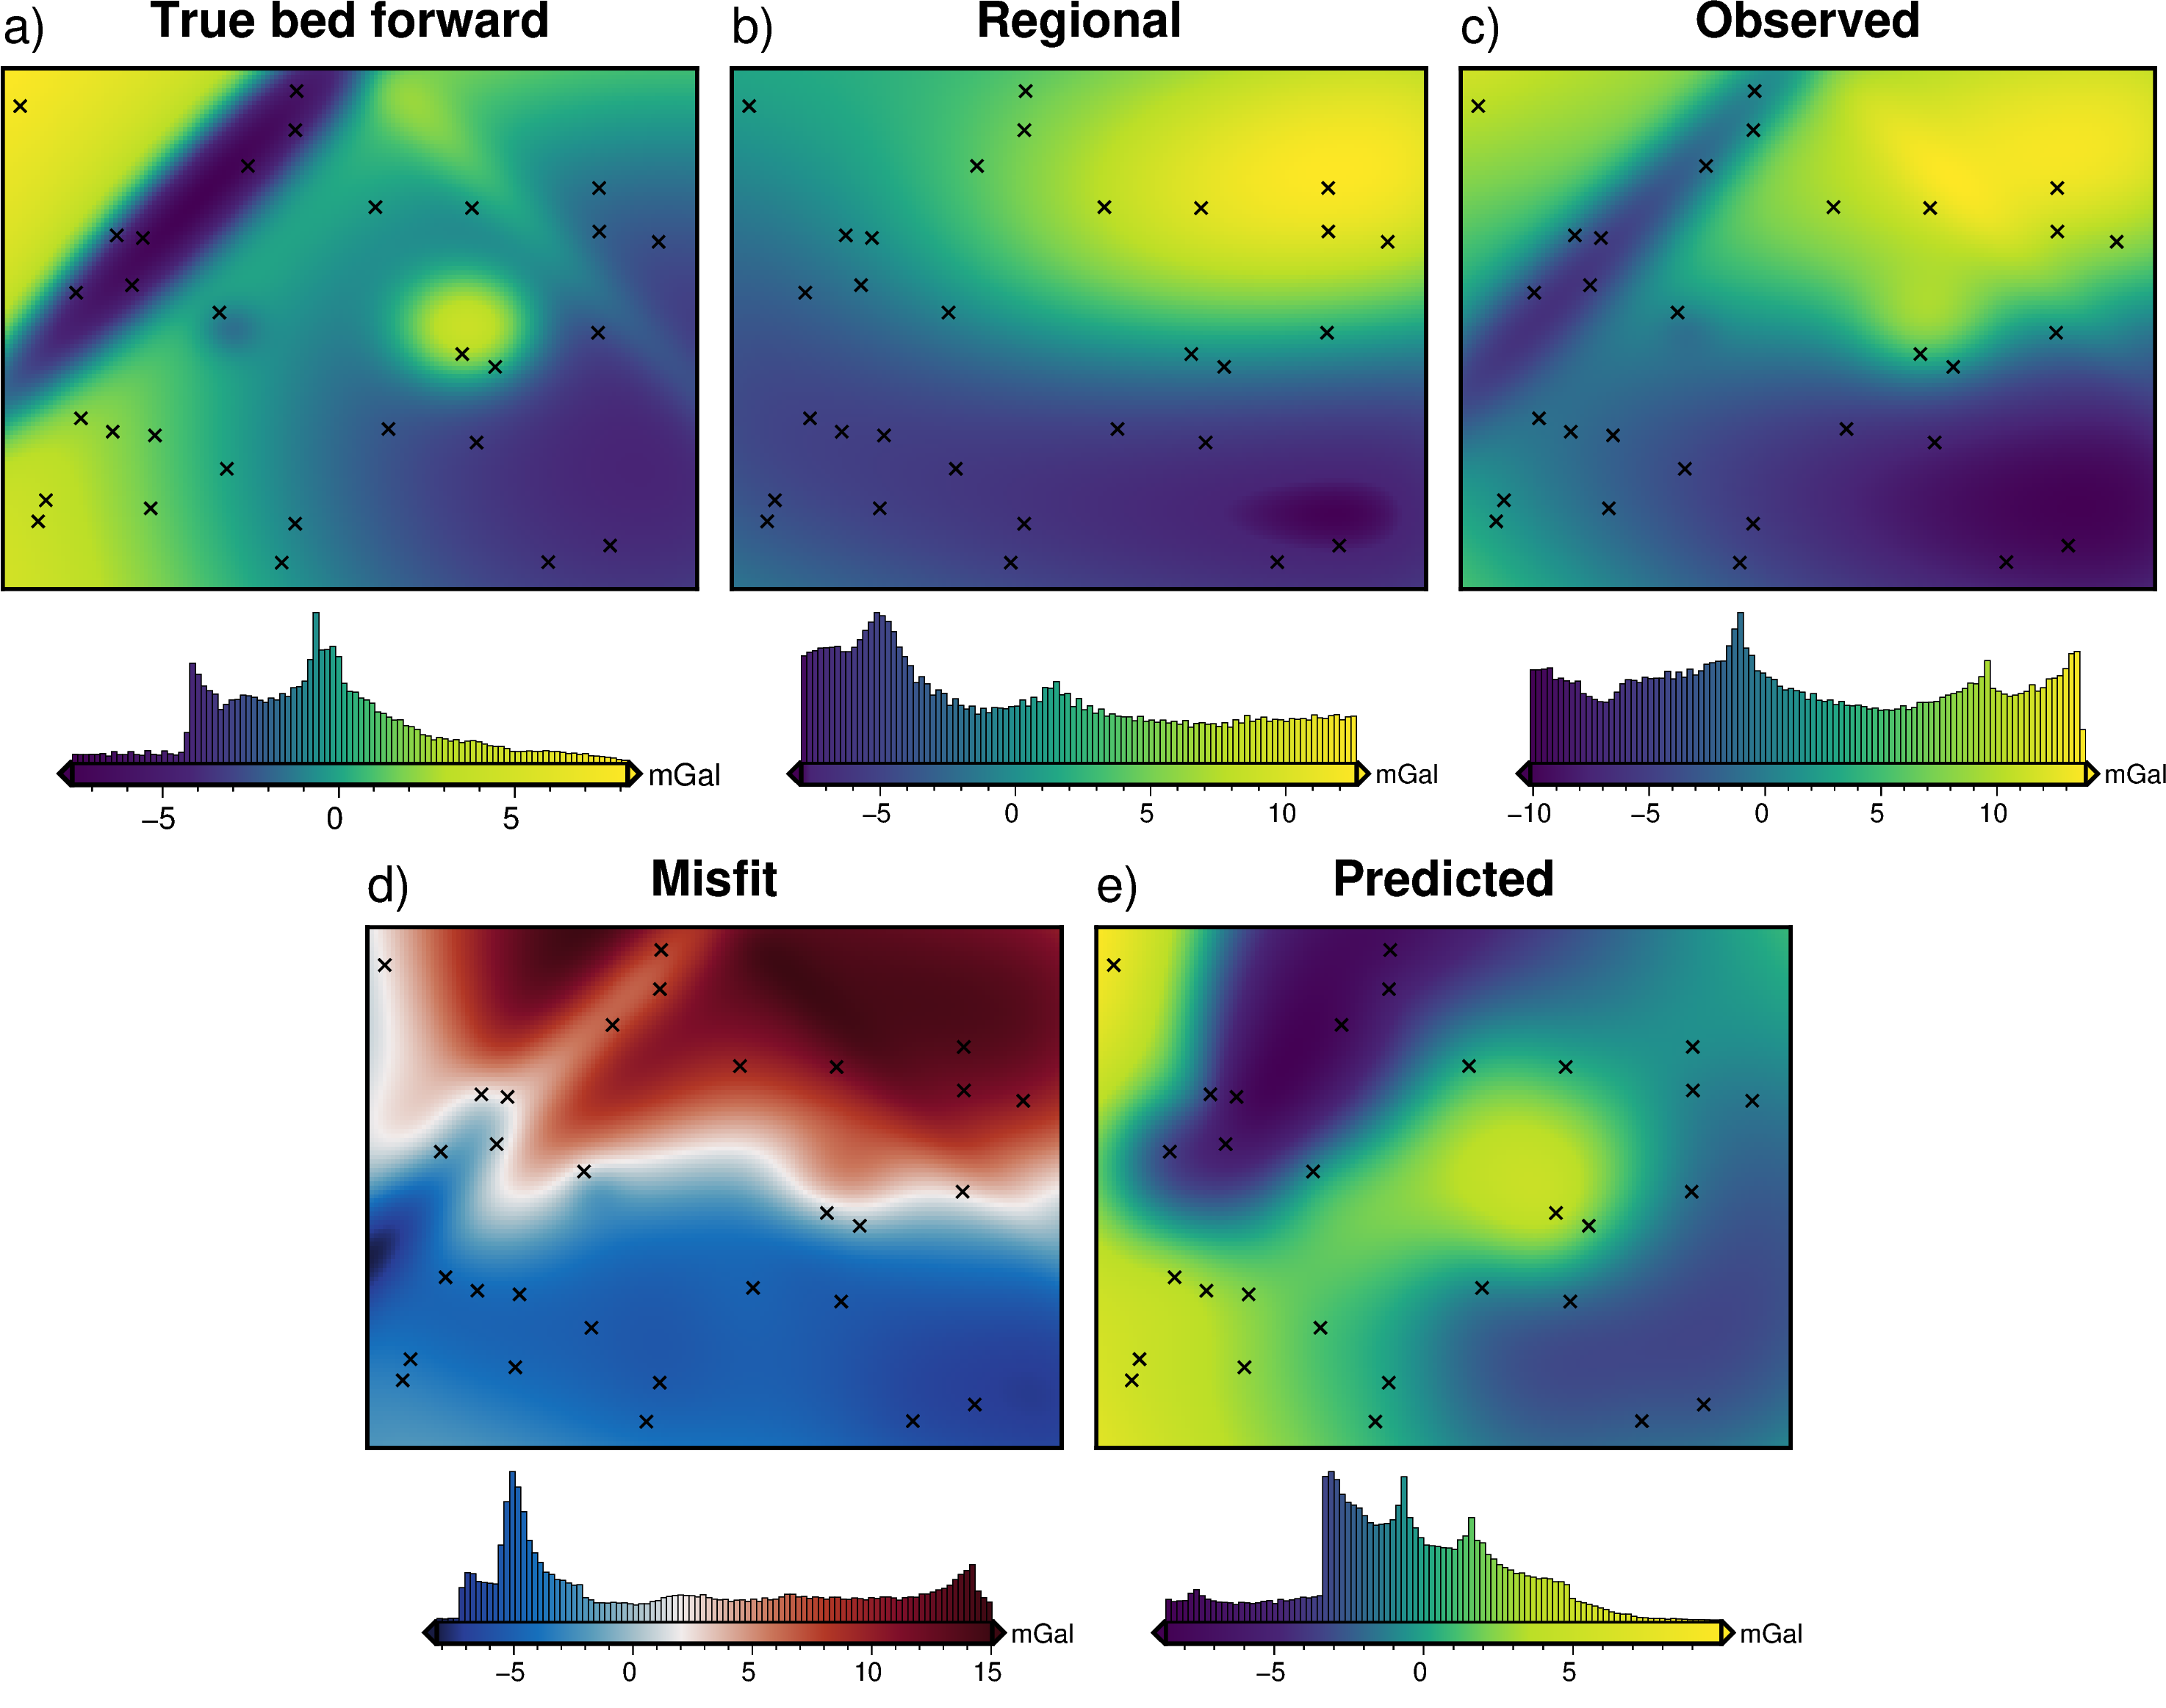
\includegraphics[width=0.95\textwidth]{figures/chp3/chp3_simple_regional_gravity.png}
    \caption[Gravity anomalies with a regional field]{Gravity components and anomalies for the simple synthetic model with the addition of a regional field. \textbf{a)} the forward gravity of the true bathymetry, \textbf{b)} the regional component of gravity, \textbf{c)} the observed gravity from the combination of a and b, \textbf{d)} the gravity misfit from the difference between c and e, and \textbf{e)} the predicted gravity from the forward calculation of the starting bathymetry.}
    \label{fig:chp3_simple_regional_gravity}
\end{figure}

This model uses the same starting bathymetry (Figure \ref{fig:chp3_simple_starting_model}) as the previous section, but the observed gravity includes a regional field, which represents the portion of observed gravity signal resulting from unknown crustal sources, such as anomalous bodies or crustal thickness variations. This component (Figure \ref{fig:chp3_simple_regional_gravity}b) is calculated from a synthetic topography with a median elevation of -4300~m and a density contrast of 700~kg~m\textsuperscript{-1}. Its range of gravity values is set to be the dominant signal in the observed gravity, but not large enough to fully mask the signal of the bathymetry signal. Figure \ref{fig:chp3_simple_regional_gravity} shows the various components of the gravity and resulting misfit for this model. 

\subsection{Regional separation methods}

The four methods of regional separation discussed in section \ref{chp3_regional_seperation} each have at least one hyper-parameter which affects their calculation of the regional field. For each method these include 
\begin{enumerate}
    \item Low-pass filter: the distance width of the Gaussian filter.
    \item Trend removal: the degree of the polynomial trend fit to the misfit.
    \item Equivalent source prediction: the depth and damping parameters of fitting sources to the data \citep{solergradientboosted2021}.
    \item Constraint point minimization: parameters for the associated gridding method, such as the tension factor for minimum curvature gridding \citep{smithgridding1990} or the minimum distance and damping parameter for bi-harmonic spline gridding \citep{uiedaverde2018}.
\end{enumerate}

\begin{figure}[!ht]
    \centering
    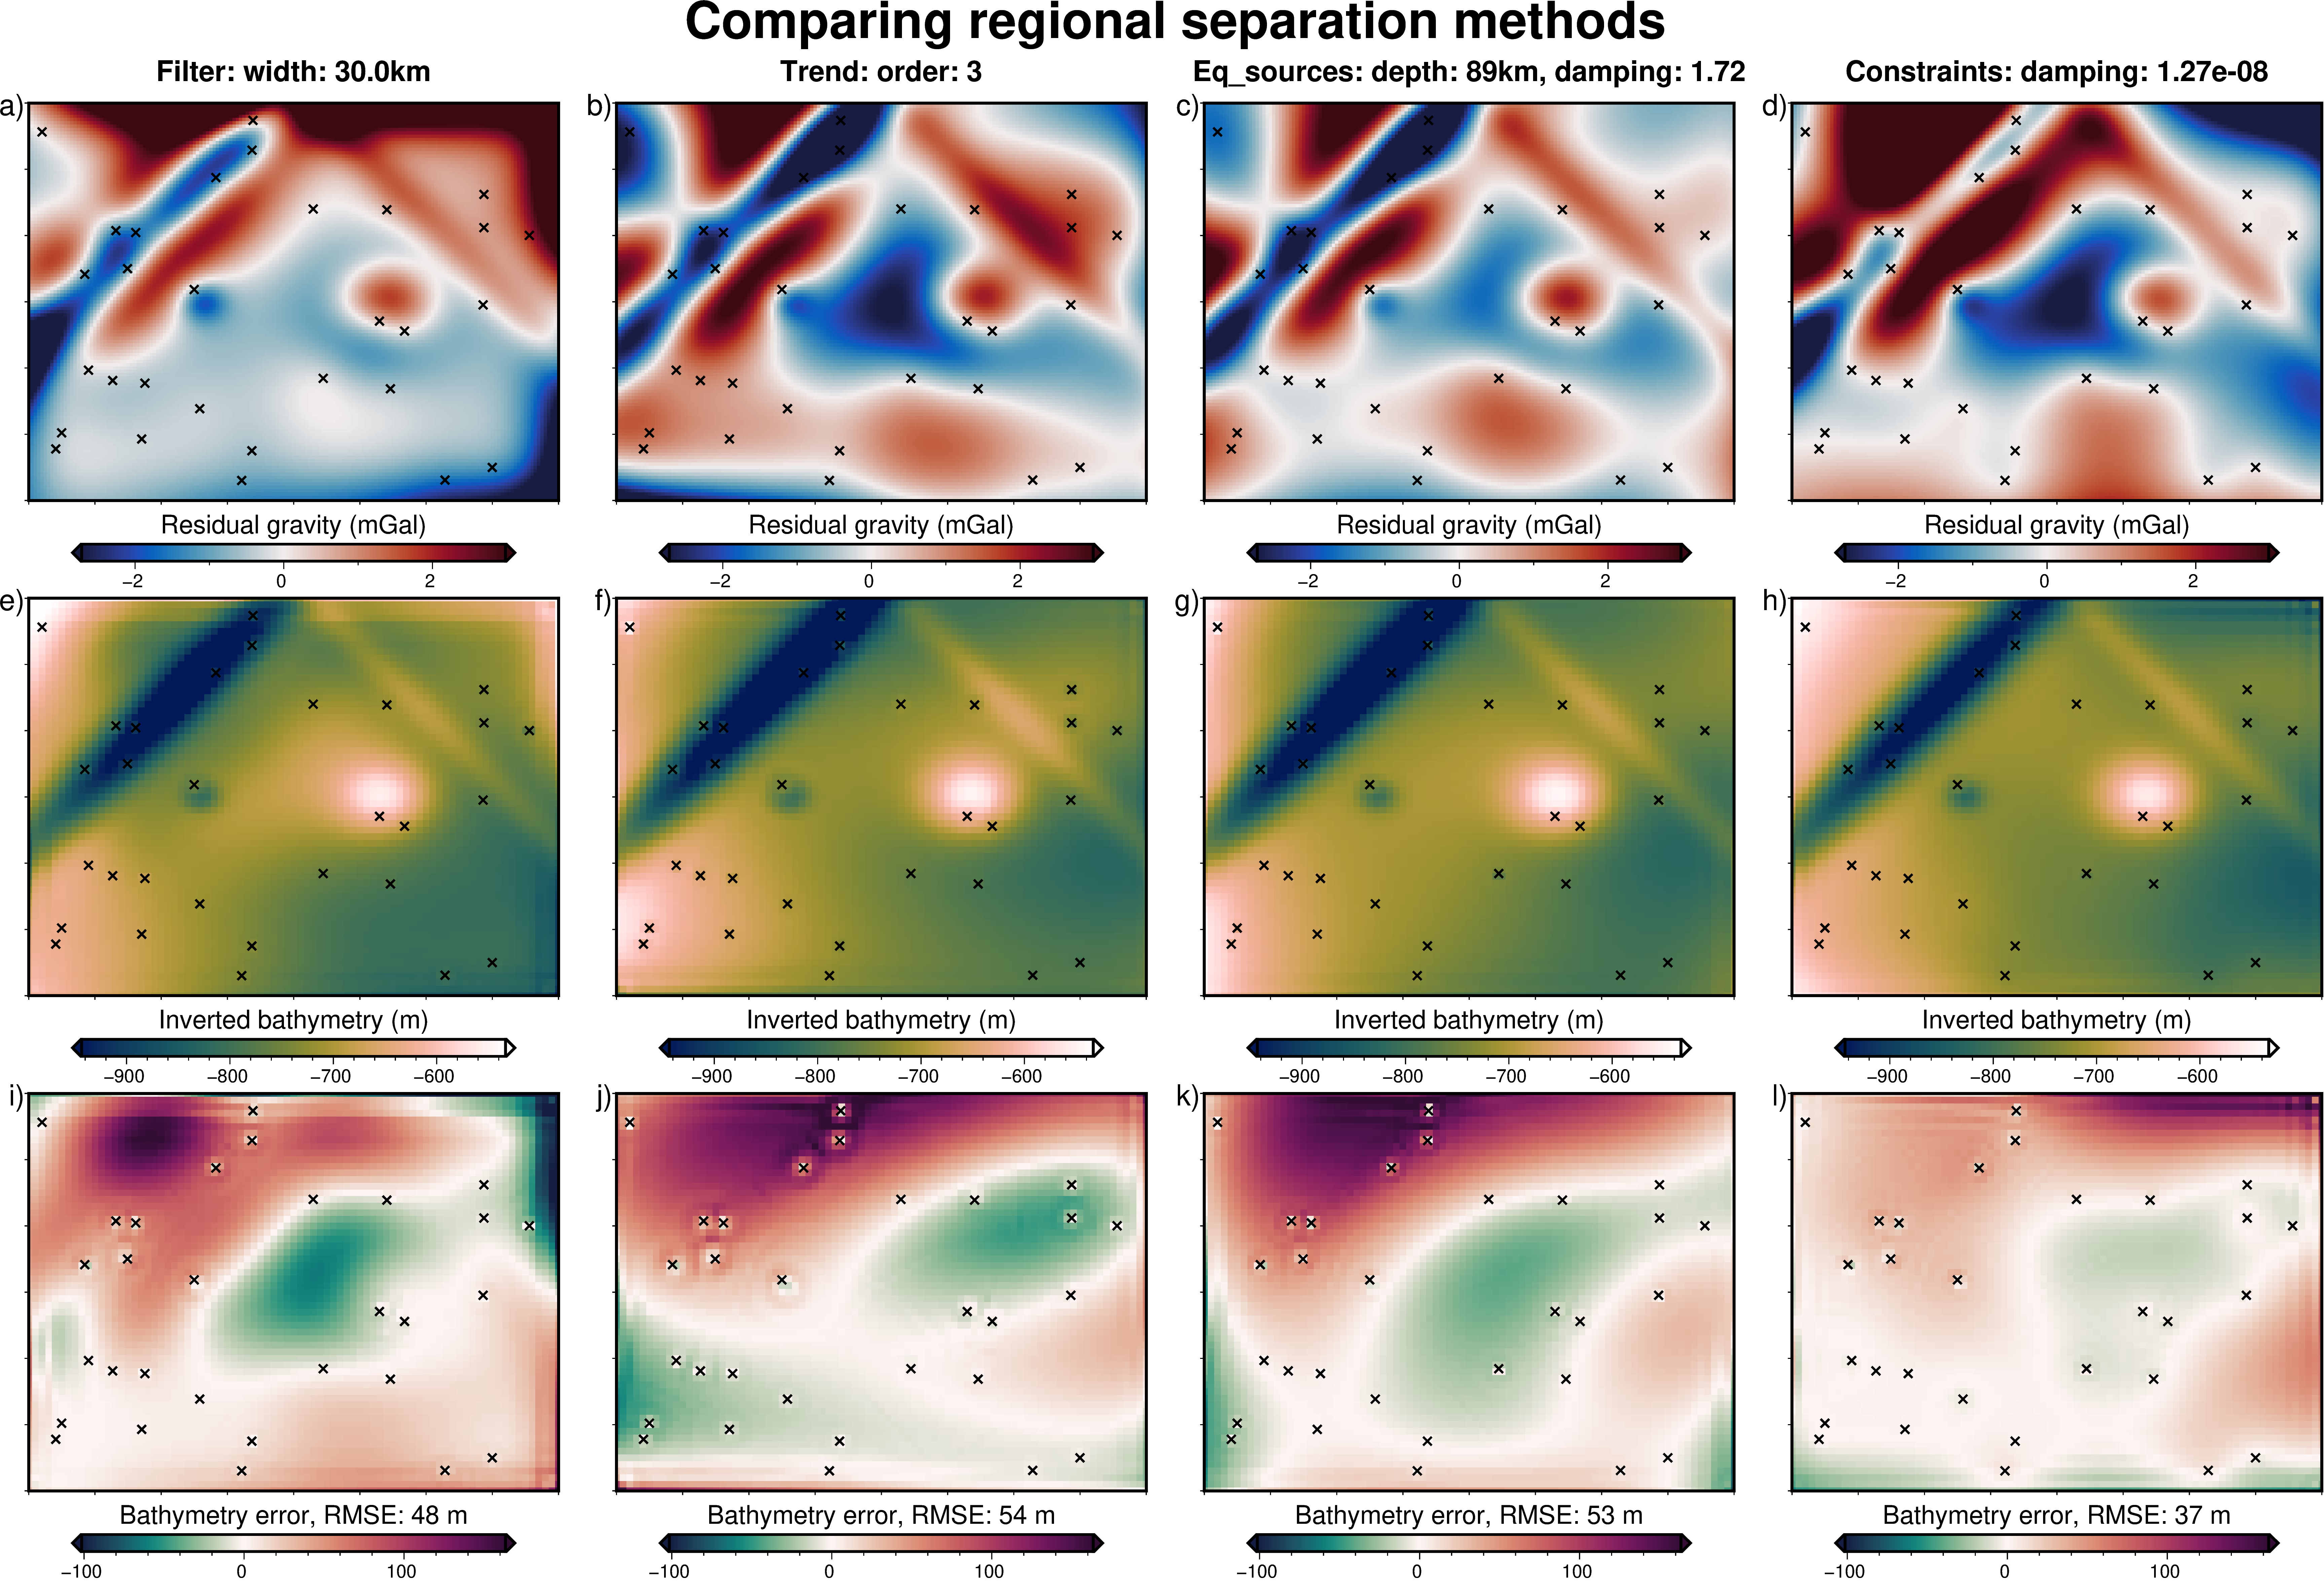
\includegraphics[width=1\textwidth]{figures/chp3/chp3_simple_regional_comparison.png}
    \caption[Regional separation methods]{Comparison of inversions with 4 regional separation methods. First row (\textbf{a-d}) shows residual gravity misfit after regional separation. Second row (\textbf{e-h}) shows the inverted bathymetry for each method. Third row (\textbf{i-l}) shows the error of the inverted bathymetries with the true bathymetry. Constraint points are shown as black crosses. Colourmaps are identical for each row. Profiles of these data are shown in Figure \ref{fig:appB_simple_regional_comparison_profile} of Appendix \ref{appendix:B}.}
    \label{fig:chp3_simple_regional_comparison}
\end{figure}

Since for this synthetic model, the true regional field is known (Figure \ref{fig:chp3_simple_regional_gravity}b), the effect of the parameters associated with each of the four methods can be explored. Excluding the constraint point minimization method, an optimization is run for each method, with the goal of finding the parameter values which minimize the RMS difference between the true and calculated regional gravity. Each optimization has 20 trials. The constraint point minimization doesn't require optimization because the various gridding parameters won't significantly affect the RMS difference between the resulting regional field and the true field. However, the gridding parameters will affect the inversion itself; this is explored in the next section. For this comparison of the regional removal method, the constraint point minimization method uses bi-harmonic spline grinding, and the gridding damping parameter is chosen with a cross-validation \citep{uiedaverde2018}. The best regional field (lowest RMS with the true regional field) of each method was found with the following parameters: 
\begin{enumerate}
    \item a 30~km filter width for the low pass filter method
    \item a 3\textsuperscript{rd} order trend for the trend removal method
    \item source depth of 89~km and a damping value of 1.72 for the equivalent source technique
    \item an interpolator damping of $1.27x10^{-8}$ for the bi-harmonic spline interpolator of the constraint point minimization method. 
\end{enumerate}

Each of these regional fields was then removed from the gravity misfit, producing the residual anomalies (Figure \ref{fig:chp3_simple_regional_comparison}a-d). These resulting residuals were then input into an inversion, resulting in the inverted bathymetries of d-h of Figure \ref{fig:chp3_simple_regional_comparison}, and the bathymetry error relative to the true bathymetry was found (Figure \ref{fig:chp3_simple_regional_comparison}i-l). For these inversions, the same damping parameter cross-validation was conducted, as described in Section \ref{chp3:simple_model_CV}. This comparison of regional separation methods shows that the constraint point minimization method (Figure \ref{fig:chp3_simple_regional_comparison}l) produces the best inverted bathymetry, both visually (Figure \ref{fig:chp3_simple_regional_comparison}h), and based on the RMS difference with the true bathymetry (37~m). Figure \ref{fig:appB_simple_regional_comparison_profile} in Appendix \ref{appendix:B} shows a profile of the resulting regional fields and inverted bathymetries of these various methods of regional separation. The remainder of this section further examines the constraint point minimization method of regional separation.

\subsection{Constraint point minimization} \label{chp3_gridding_comparison}
The constraint point minimization method assumes that at locations of known bathymetry, there is no residual component of gravity misfit, and the regional component entirely equals the misfit. To implement this, misfit values at the constraints are sampled and used to create a region-wide grid of regional values. This grid is then removed from the misfit to get the residual misfit (Equation \ref{eq:regional_residual}). This gridding can be accomplished by many techniques, which at an initial inspection appear to produce similar results. Here, two methods of gridding and their gridding parameters are compared, and the impact on the inverted bathymetry are shown. These gridding methods are tensioned minimum curvature \citep{smithgridding1990} and bi-harmonic splines \citep{sandwellbiharmonic1987}. 

\subsubsection{Tensioned minimum curvature}
Tensioned minimum curvature gridding is a commonly used technique for gridding sparse data which fits the smoothest possible surface while still matching the data \citep{wesselinterpolation1998}. It allows variation in the location of maximum curvature through the tension factor parameter. A tension factor of 0 results in the minimum curvature solution (maxima and minima allowed anywhere), while a value of 1 localizes the curvature at the data points (maxima or minima only allowed at the data points) \citep{smithgridding1990}. A tension of 0.25 is suggested for potential field data \citep{wesselgeneric2019}. Tensioned minimum curvature has been used in several bathymetric inversions for constraint point minimization \citep{yangbathymetry2021, millanconstraining2020, anbathymetry2019}. 

\subsubsection{Bi-harmonic splines}
The second method of gridding the sampled gravity misfit values uses bi-harmonic splines. This method uses Green's functions and the least squares fit to the data \citep{sandwellbiharmonic1987}. Computation time for this technique is approximately proportional to the cube of the number of data, making it computationally expensive for large datasets \citep{dengmoving2011}. There is a damping parameter value that can be adjusted, to smooth the resulting interpolation. As implemented in the \textit{SplineCV} class of the Python package Verde \citep{uiedaverde2018}, automated cross-validation of the data can be used to identify the damping value which  best predicts the data. Once the parameter is determined, and the data is interpolated, the interpolation can be predicted at any location, such as on the nodes of a uniform grid. \\

Despite its slow run time with large datasets, bi-harmonic spline gridding has several advantages over tensioned minimum curvature gridding. It allows the incorporation of data uncertainties into the fitting via a weighting parameter. With the use of cross-validation, there are no subjective parameters that can significantly alter the results. Lastly, the predicted data don't need to be on a regular grid, which is useful for irregularly shaped domains that don't adhere to a rectangular region. In their bathymetry inversion, \citet{millanconstraining2020} point out features in their inverted bathymetry which likely result from the minimum curvature gridding technique. Apart from this, there appears to be little work related the how the gridding procedure affects this aspect of a bathymetry inversion.

\begin{figure}[!ht]
    \centering
    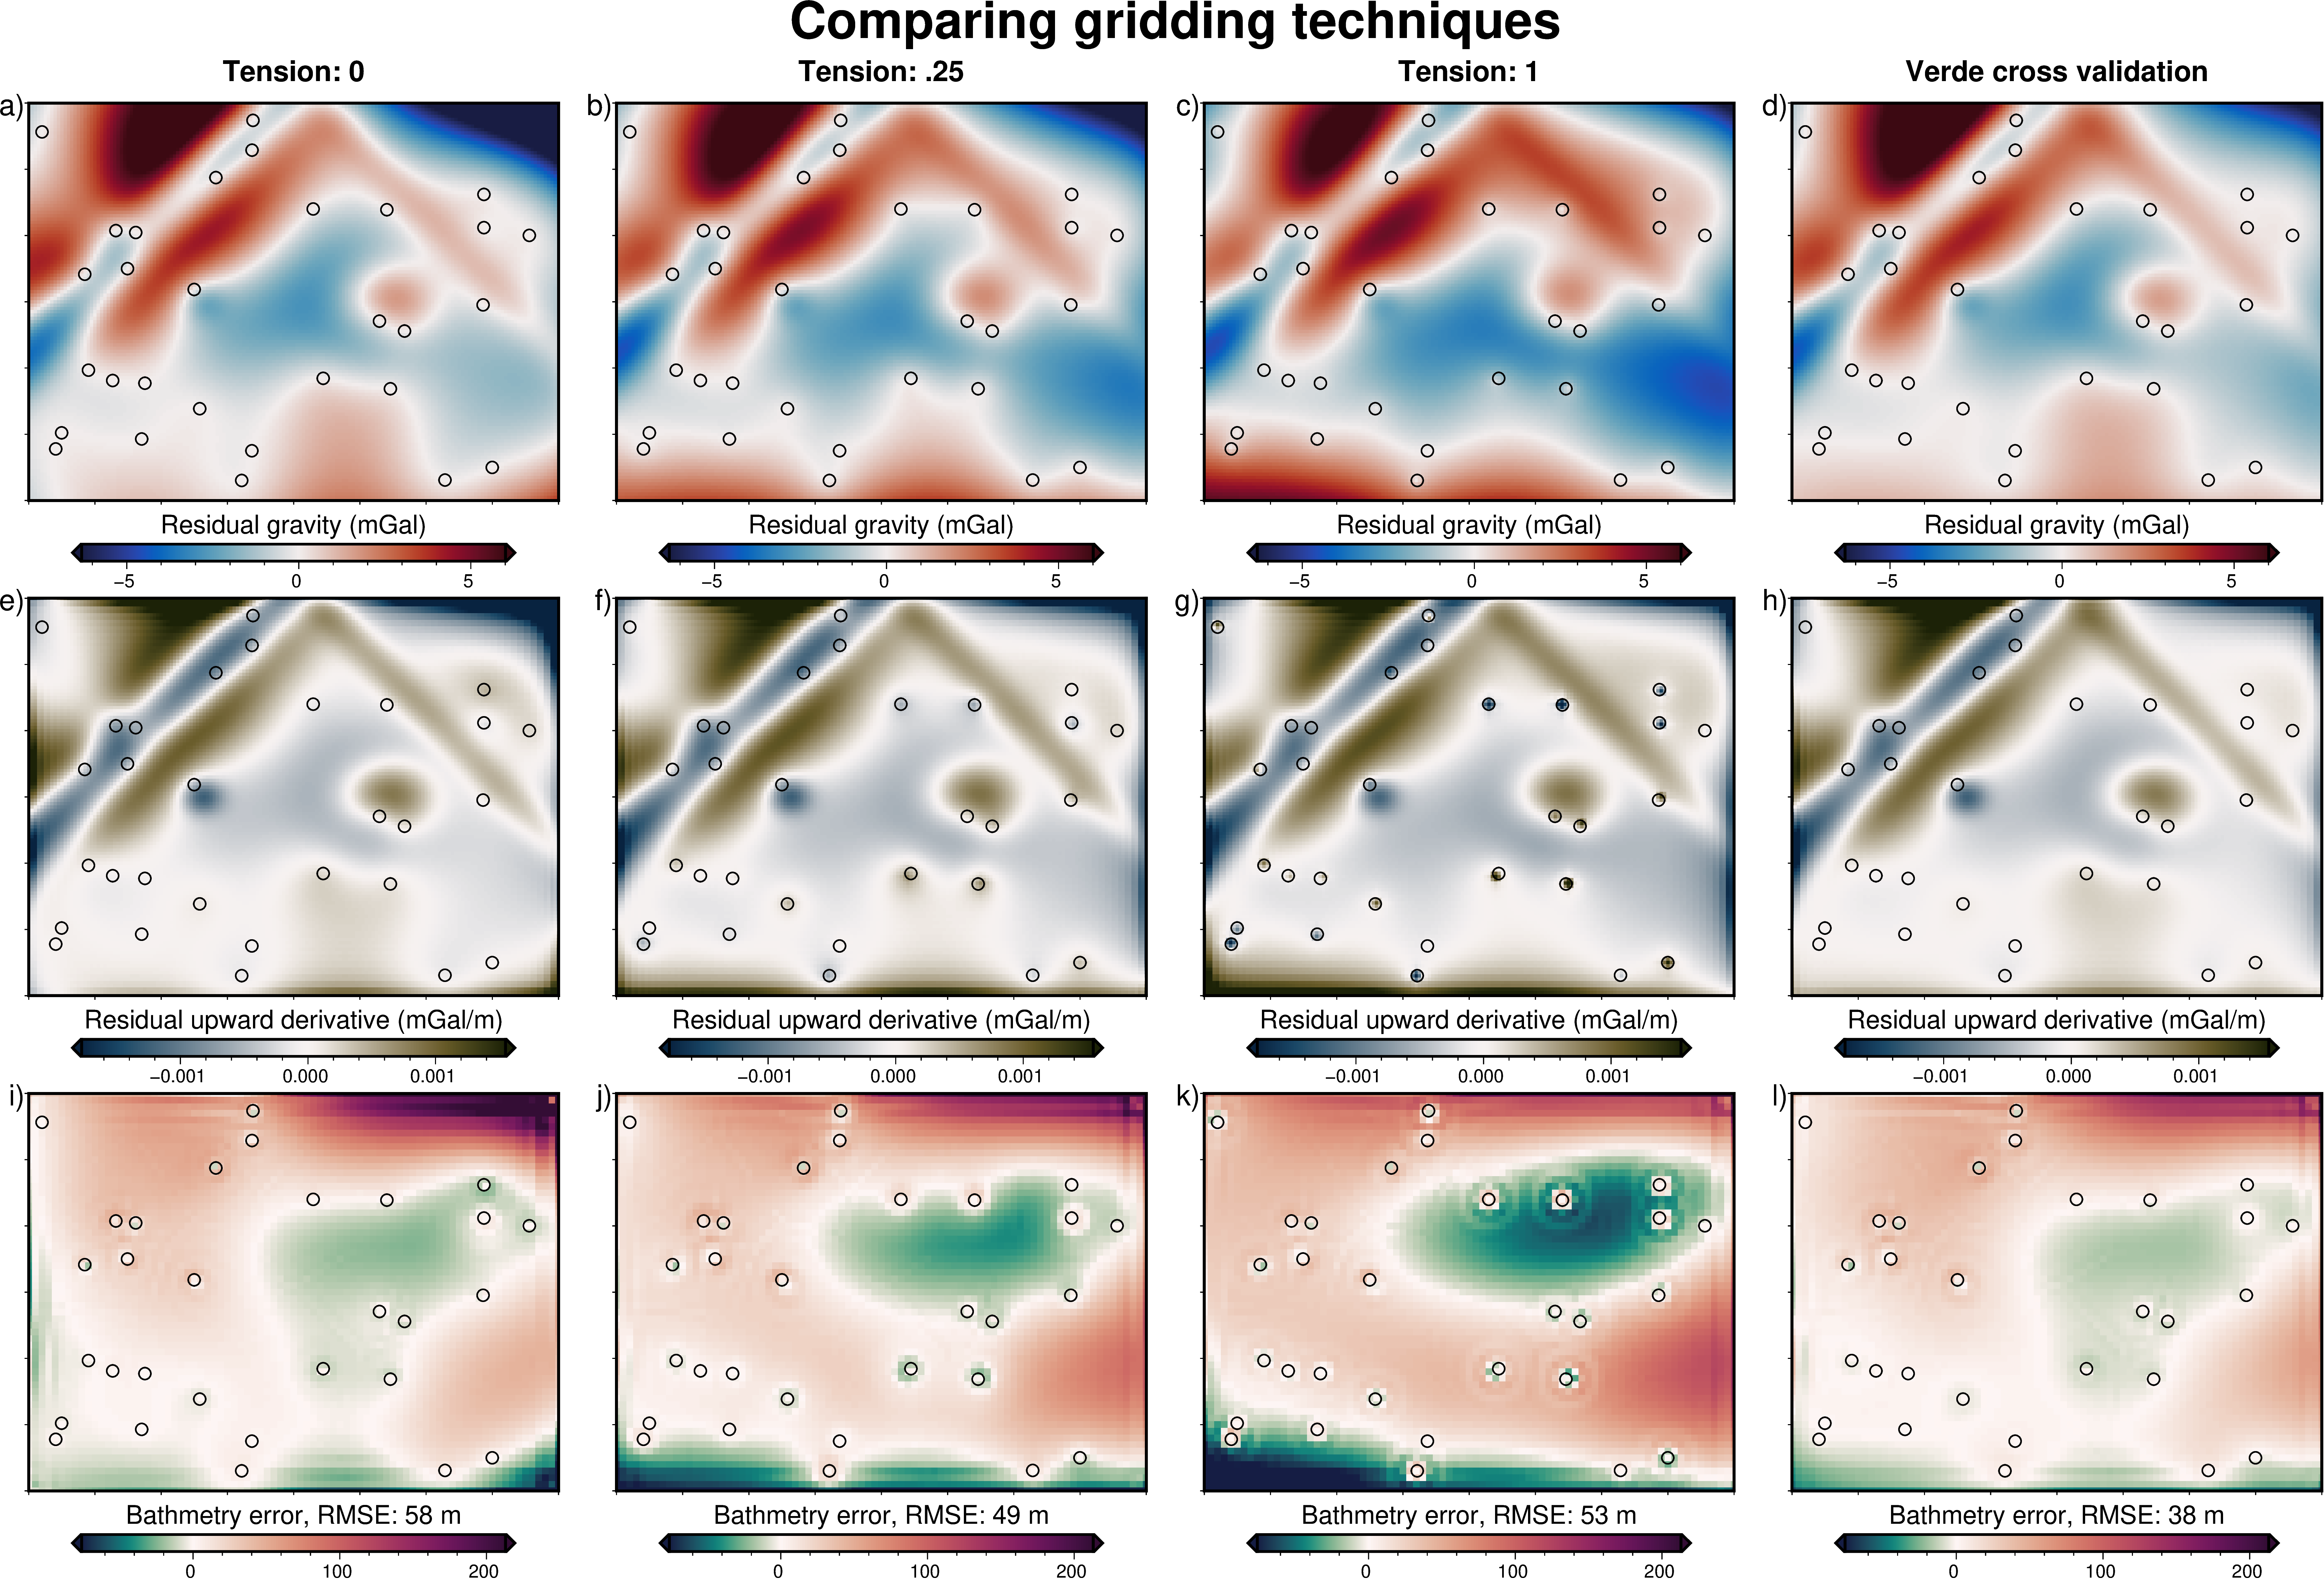
\includegraphics[width=1\textwidth]{figures/chp3/chp3_simple_regional_gridding_comparison.png}
    \caption[Constraint point minimization gridding techniques]{Comparison of gridding techniques for the constraint point minimization method of regional-residual separation. By sampling the misfit at constraints, and re-gridding over the entire domain, the regional component of the misfit is estimated. Gridding methods include minimum curvature gridding with tension factors of 0 (\textbf{column 1}), 0.25 (\textbf{column 2}), 1 (\textbf{column 3}), and cross-validated bi-harmonic spline gridding (\textbf{column 4}). Resulting gridded regional components were removed from the misfit grids to produce the residual grids (\textbf{a-d}). Second row (\textbf{e-h}) shows the vertical derivative of the residual, to highlight the gridding variations. Third row (\textbf{i-l}) shows the error of the inverted bathymetries with the true bathymetry. Constraint points are shown as open circles. Colourmaps are identical across all columns. Profiles of these data are shown in Figure \ref{fig:appB_simple_regional_gridding_comparison_profile} of Appendix \ref{appendix:B}.}
    \label{fig:chp3_simple_regional_gridding_comparison}
\end{figure}

\subsubsection{Gridding comparison}

In this section, the effect which the gridding process has on the inverted bathymetry is analyzed. Four sets of regional separations were conducted, three using the tensioned minimum curvature technique, and one using the bi-harmonic spline technique. For the three minimum curvature separations, the tension factors used were the end members, 0 and 1, and the suggested value for geopotential data, 0.25. For the bi-harmonic spline, a cross-validation with 20 varying damping values was conducted, and the best resulting damping value was used. For each of the four calculated regional fields, the resulting residual fields (Figure \ref{fig:chp3_simple_regional_gridding_comparison}a-d) were used as inputs to an inversion. All four residual anomaly data were included in an inversion damping parameter cross-validation, as described in Section \ref{chp3:simple_model_CV}. The difference between the resulting inverted bathymetry and the true bathymetry of each model is shown in Figure \ref{fig:chp3_simple_regional_gridding_comparison}i-l. To help visualize the difference in the resulting residual grids, \ref{fig:chp3_simple_regional_gridding_comparison}e-h shows the vertical derivative of the residual fields. This highlights that while the residual values at the constraints are all similar, the slope of the residual in the vicinity of the grids is strongly dependent on the gridding method \footnote{Note that the gridding process creates the regional field (not shown in Figure \ref{fig:chp3_simple_regional_gridding_comparison}), which when subtracted from the total misfit gives the residual field. The residual grid is affected by these gridding effects through the removal of the regional field.}. Additionally, the minimum curvature gridding is shown, in subplots a-c, to create large artificial anomalies away from constraint points (low values in upper right corners). These gridding artifacts result in large errors in the resulting bathymetry \ref{fig:chp3_simple_regional_gridding_comparison}i-k. The bi-harmonic spline interpolator (last column in \ref{fig:chp3_simple_regional_gridding_comparison}) is shown to produce a residual field that adheres to the constraints, has smooth curvature near constraints, and doesn't create large artificial anomalies. The effectiveness of this interpolator is confirmed by the low RMS difference between the inverted and true bathymetry (38~m). Figure \ref{fig:appB_simple_regional_gridding_comparison_profile} in Appendix \ref{appendix:B} shows a profile of the resulting regional fields and inverted bathymetries of these various gridding methods. With the bi-harmonic spline gridding techniques shown to be the most effective, the remainder of this chapter uses this gridding technique for the constraint point minimization method of regional separation.

\begin{figure}[!ht]
  \centering
    \begin{subfigure}[t]{.40\textwidth}
        \centering
        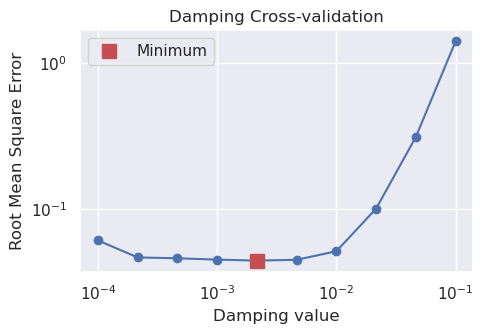
\includegraphics[width=\textwidth]{figures/chp3/chp3_simple_regional_CV.png}
        \caption{}
    \end{subfigure}
    \begin{subfigure}[t]{.58\textwidth}
        \centering
        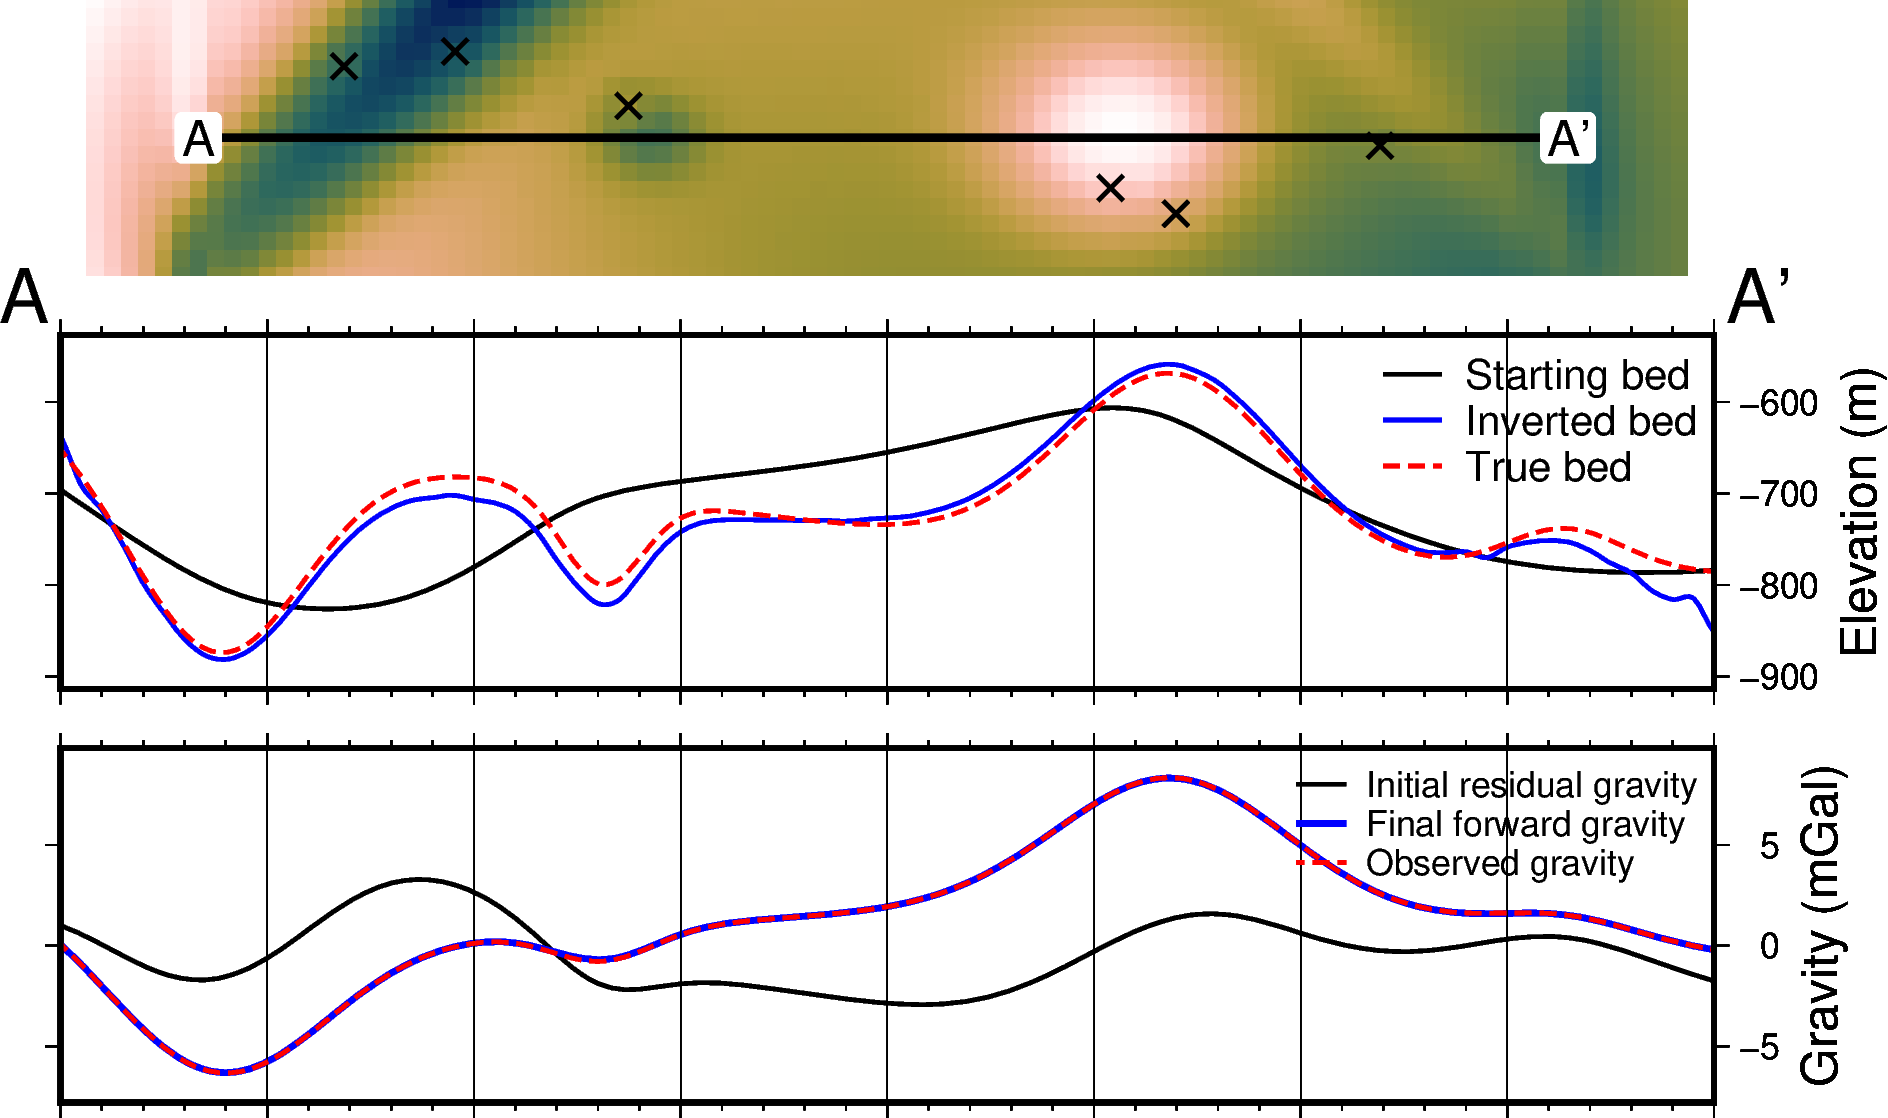
\includegraphics[width=\textwidth]{figures/chp3/chp3_simple_regional_profile.png}
        \caption{}
    \end{subfigure}
  \caption[Synthetic inversion with regional component, CV and profile]{Cross-validation and profiles for the simple synthetic inversion with a regional component removed. \textbf{a)} Cross-validation curve showing the optimal damping parameter (red square). \textbf{b)} 2D profile of the inversion results. The top panel shows profile location and constraint points (black crosses). The middle panel contains topographic profiles of the starting, inverted, and true bathymetries. The bottom panel contains gravity anomaly profiles.}
    \label{fig:chp3_simple_regional_CV_and_profile}
\end{figure}

\subsection{Inversion results}

\begin{figure}[!ht]
    \centering
    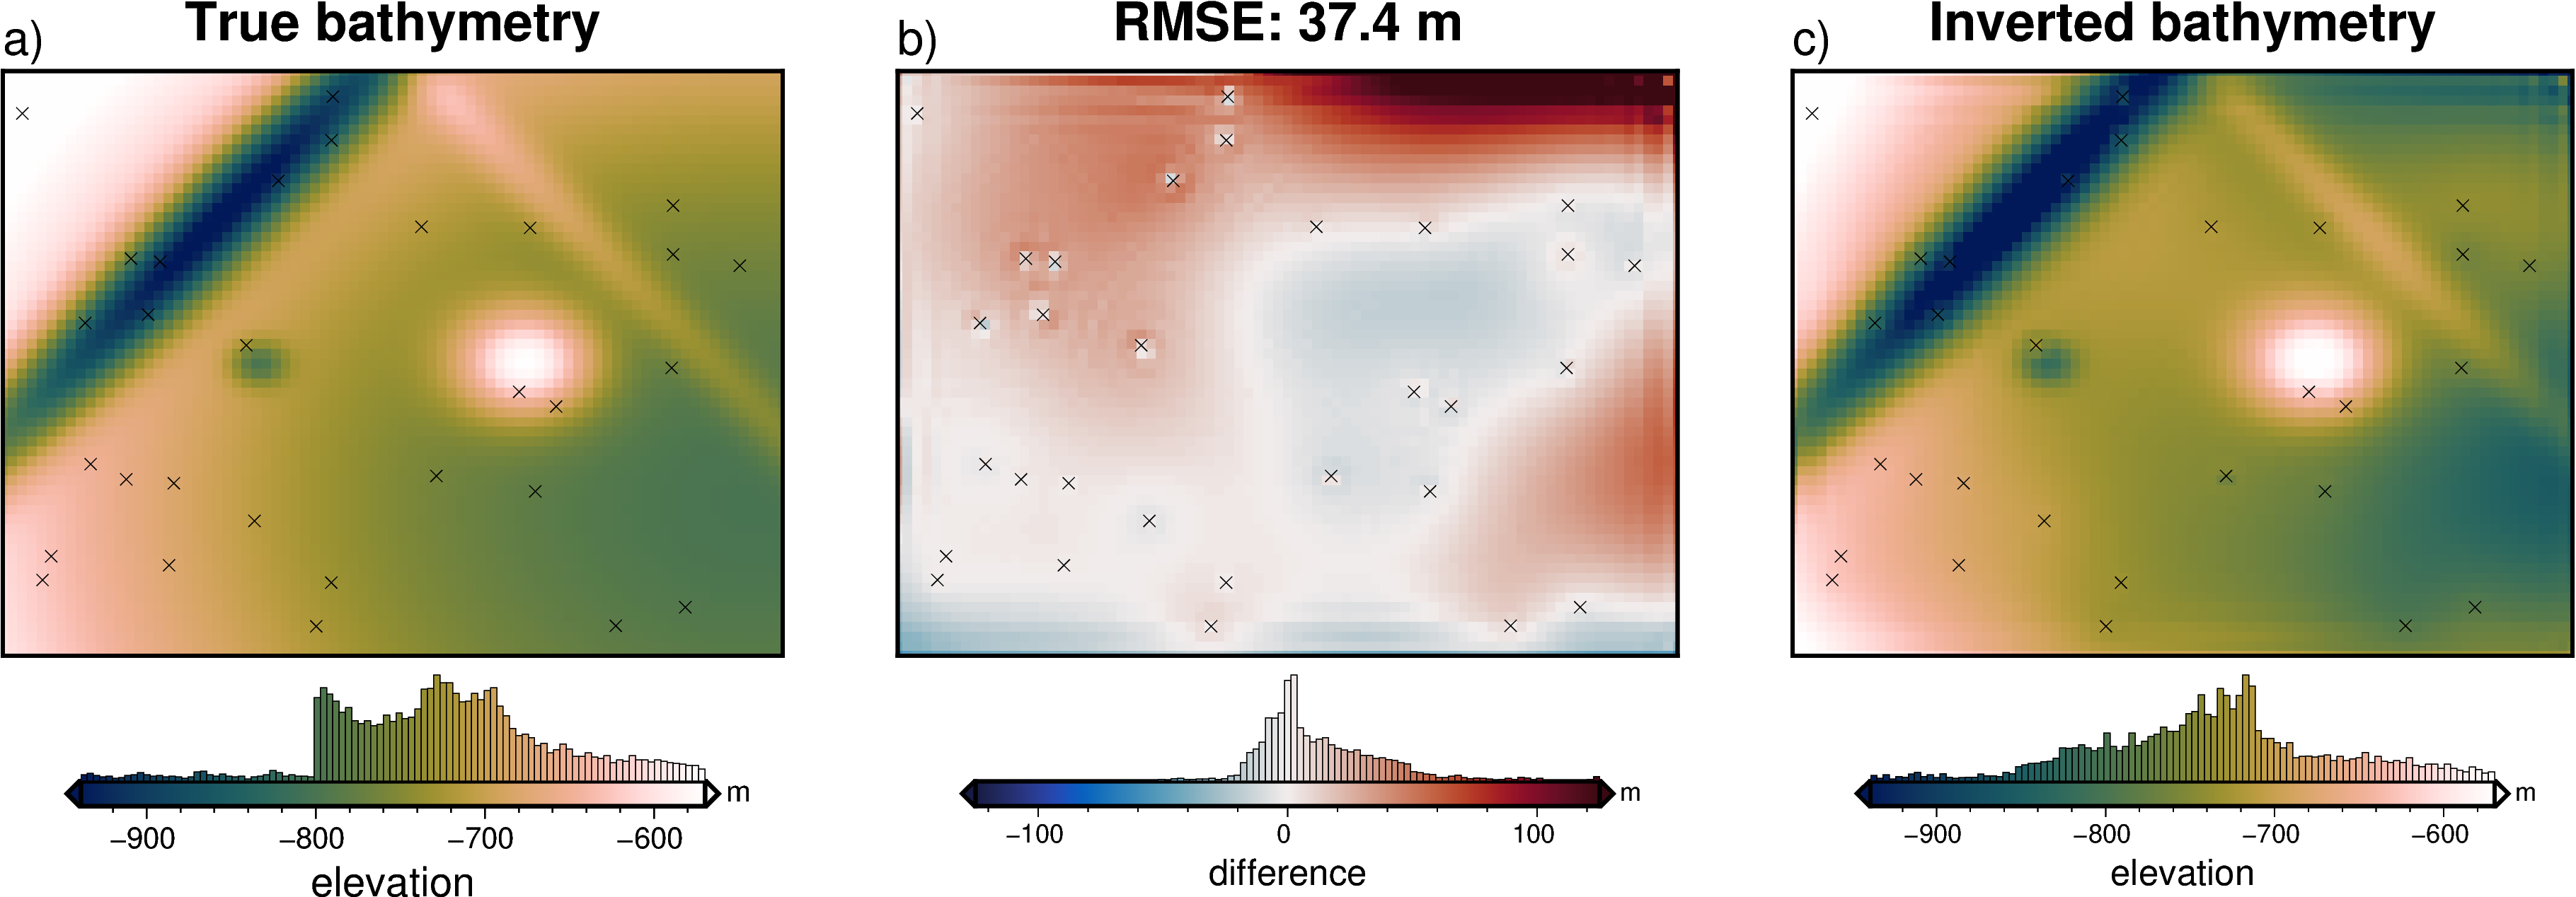
\includegraphics[width=.95\textwidth]{figures/chp3/chp3_simple_regional_results.png}
    \caption[Synthetic inversion with regional component results]{Simple synthetic model inversion with a removed regional component. \textbf{a)} True bathymetry, \textbf{b)} difference between a and c, \textbf{c)} final inverted bathymetry. Black crosses are constraint points. The RMS difference with the true bathymetry at these constraints is 2~m.}
    \label{fig:chp3_simple_regional_results}
\end{figure}

Using the cross-validated bi-harmonic gridding method to separate the regional component of the gravity misfit, the resulting residual misfit was used in an inversion. The same gravity data cross-validation method of determining the optimal damping parameter is used (Figure \ref{fig:chp3_simple_regional_CV_and_profile}). The optimal damping parameter was found to be $\sim10^{-2.6}$. The resulting inversion is shown in Figure \ref{fig:chp3_simple_regional_results}. The inverted bathymetry had an RMS difference with the true bathymetry of 37~m and an RMS difference at the constraints of 2~m. The inversion was completed in 66 seconds, with 39 iterations and a final RMS residual of 0.022~mGal. The inversion was terminated due to the $\ell^2$-norm decreasing below the set threshold of 0.15~mGal\textsuperscript{1/2}. All four bathymetric features were recovered, but a lack of constraints in a few regions (the upper-right corner) lead to a miscalculation of the regional field and a subsequent over-deepening of the bathymetry. 

The regional separation, parameter cross-validation, and inversion were repeated with additive noise and re-sampling of the gravity data to a coarser resolution (Appendix \ref{appendix:B:simple_regional_inversion}). As in section \ref{chp3:simple_ensemble}, this above workflow was also repeated for an ensemble of noise levels and gravity data grid spacings, as discussed next. 

\subsection{Ensemble of Noise and Sampling values} \label{chp3:simple_regional_ensemble}

Following the method outlined in Section \ref{chp3:simple_ensemble}, an ensemble of 100 inversions with varying levels of noise and gravity observation spacings was conducted. The noise and gravity spacing changes were applied to the original observed data, and the forward calculation of the starting model, initial misfit calculation, and regional field removal were all repeated. Each model was then inverted with a cross-validation, and the resulting RMS differences with the true bathymetry are shown in Figure \ref{fig:chp3_simple_regional_ensemble}. 

\begin{figure}[!ht]
    \centering
    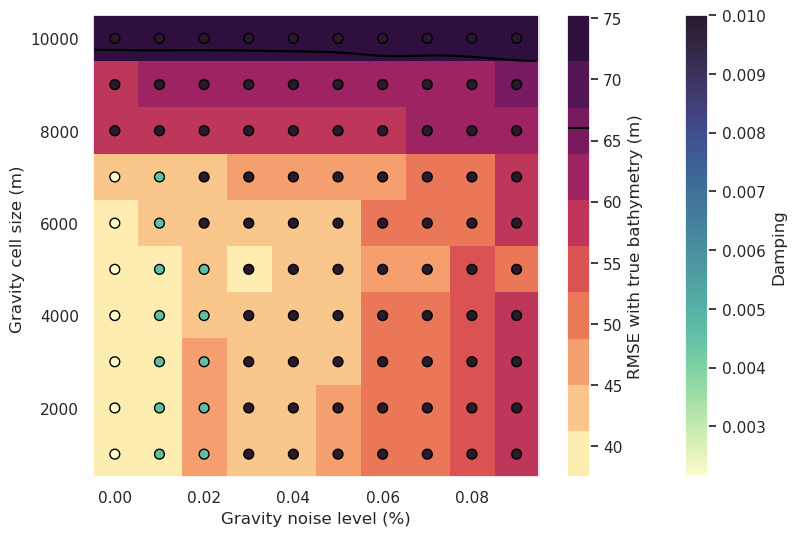
\includegraphics[width=0.9\textwidth]{figures/chp3/chp3_simple_regional_ensemble.png}
    \caption[Gravity data ensemble with regional component]{Ensemble of noise levels and gravity spacing for the simple synthetic model with a regional field. Grid cell colour indicates each inversion's RMSE with the true bathymetry. The circles' colour indicates the optimal damping value found for each inversion's cross-validation. Black line shows the 66~m contour, representing the RMS difference between the true and starting bathymetry.}
    \label{fig:chp3_simple_regional_ensemble}
\end{figure}

\subsection{Simple model comparison}

Table \ref{table:chp3_simple_synthetic_stats} compares the performance of each of the above inversions. The four inversions without a regional component of the gravity data (annulus approximation, prism approximation, with noise, and resampled), all recovered the bathymetry with an RMSE of $\sim$~10~m. With the regional component, the lowest RMS was raised to 37~m. The constraint point minimization method of regional separation produced significantly more accurate bathymetry models than the other methods. With these optimal methods and baseline performance standards, a new synthetic model is introduced which was created to emulate the expected bathymetry features and gravity anomalies associated with a sub-ice-shelf environment.

% Please add the following required packages to your document preamble:
% \usepackage{graphicx}
\begin{table}[]
\resizebox{\textwidth}{!}{%
\begin{tabular}{l|ccccc}
\multicolumn{1}{c|}{}            & \begin{tabular}[c]{@{}c@{}}RMS \\ (m)\end{tabular} & \begin{tabular}[c]{@{}c@{}}RMS at constraints \\ (m)\end{tabular} & \begin{tabular}[c]{@{}c@{}}Total time \\ (hr:min:sec)\end{tabular} & \# iterations        & \begin{tabular}[c]{@{}c@{}}Final residual RMS \\ (mGal)\end{tabular} \\ \hline
\textbf{No regional component}   & \multicolumn{1}{l}{}                               & \multicolumn{1}{l}{}                                              & \multicolumn{1}{l}{}                                               & \multicolumn{1}{l}{} & \multicolumn{1}{l}{}                                                 \\
Starting bathymetry              & 66                                                 & 0.04                                                              & –                                                                  & –                    & 2.7                                                                  \\
annulus                          & 8                                                  & 1                                                                 & 00:00:30                                                           & 37                   & 0.022                                                                \\
finite differences               & 9                                                  & 1                                                                 & 00:02:49                                                           & 37                   & 0.022                                                                \\
2\% noise                        & 12                                                 & $< 1$                                                             & 00:00:13                                                           & 18                   & 0.16                                                                 \\
6~km re-grid                     & 11                                                 & 1                                                                 & 00:00:29                                                           & 38                   & 0.019                                                                \\ \hline
\textbf{With regional component} &                                                    &                                                                   &                                                                    &                      &                                                                      \\
Starting bathymetry              & 66                                                 & 0.04                                                              & –                                                                  & –                    & 7.4                                                                  \\
filter                           & 48                                                 & –                                                                 & –                                                                  & –                    & –                                                                    \\
trend                            & 54                                                 & –                                                                 & –                                                                  & –                    & –                                                                    \\
equivalent sources               & 53                                                 & –                                                                 & –                                                                  & –                    & –                                                                    \\
constraint point minimization    & 37                                                 & 2                                                                 & 00:01:06                                                           & 39                   & 0.022                                                                \\
2\% noise                        & 45                                                 & 2                                                                 & 00:00:12                                                           & 13                   & 0.23                                                                 \\
4~km re-grid                     & 38                                                 & 2                                                                 & 00:00:51                                                           & 38                   & 0.022                                                               
\end{tabular}%
}
\caption[Simple synthetic model summary]{Summary of the simple synthetic model inversion results.}
\label{table:chp3_simple_synthetic_stats}
\end{table}



\section{Ross Sea model} \label{chp3:Ross_Sea}

Here a semi-realistic model is introduced. In the past section, two synthetic topographies (bathymetry and a crustal layer) were used in forward modelling to create synthetic gravity data. Here, real topographic data are used to create the synthetic gravity. This model is termed semi-realistic since the gravity is synthetically calculated, but it results from geologically real surfaces. This model uses data from Antarctica's Ross Sea (Figure \ref{fig:chp3_ice_shelves}, north of Ross Ice Shelf). The bathymetry data are from the IBCSO v2 data compilation \citep{dorschelinternational2022}, resampled at a 5~km resolution (Figure \ref{fig:chp3_Ross_Sea_layers_and_forwards}a). This data are mostly from shipborne multi-beam echo sounding. To create the regional component of gravity, basement depths from the ANTOSTRAT compilation of shipborne seismic data have been used \citep{brancolinidescriptive1995}, at a 5 km resolution (Figure \ref{fig:chp3_Ross_Sea_layers_and_forwards}b). The inversion domain is 320~$\times$~420~km and a buffer zone of 40~km was included in all directions, resulting in 8000 grid cells per surface. \\

\begin{figure}[!ht]
    \centering
    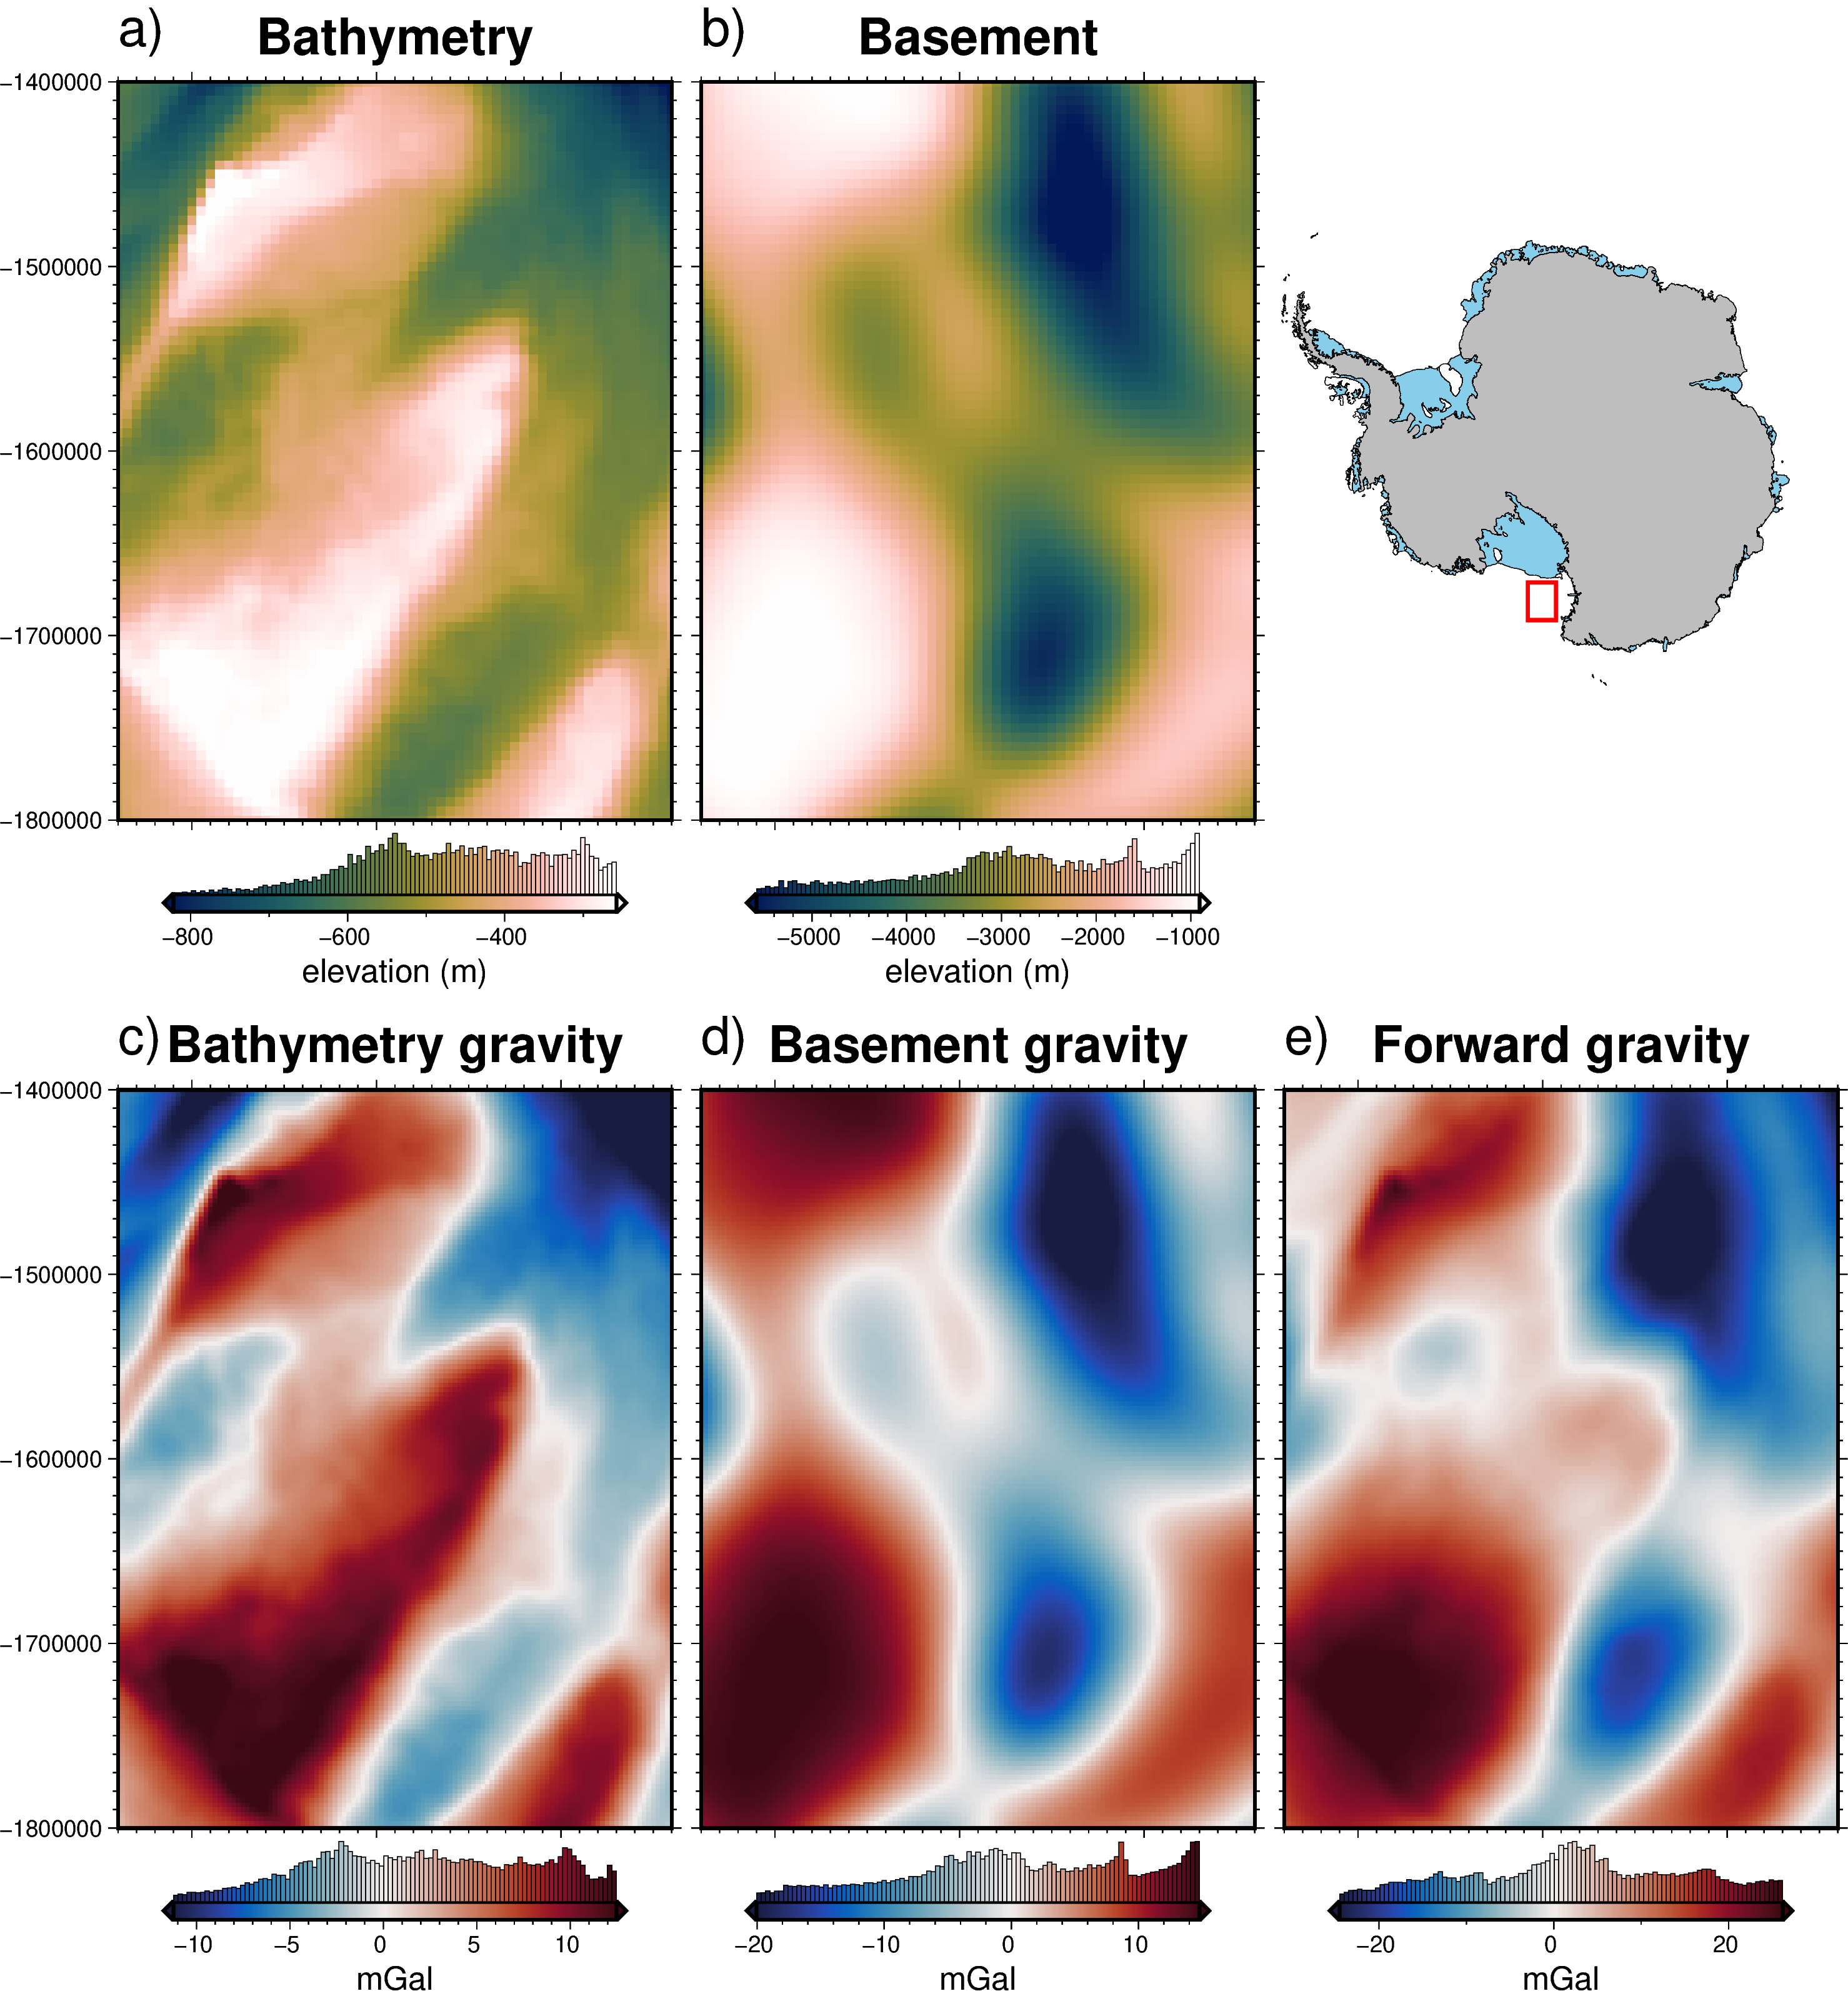
\includegraphics[width=0.95\textwidth]{chp3/chp3_Ross_Sea_layers_and_forwards.png}
    \caption[Ross Sea semi-synthetic model]{Ross Sea semi-synthetic model. \textbf{a)} Bathymetry data at 5~km resolution from IBCSO v2 \citep{dorschelinternational2022}, \textbf{b)} basement topography from the ANTOSTRAT project at 5~km resolution \citep{brancolinidescriptive1995}, \textbf{c)} forward gravity calculated at a regular 5~km grid at 1~km altitude for the bathymetry and \textbf{d)} for the basement. \textbf{e)} Total forward gravity from the combinations of c and d. Location of Ross Sea inversion domain shown as red box.}
    \label{fig:chp3_Ross_Sea_layers_and_forwards}
\end{figure}

\subsection{Observed gravity}

The bathymetric and crustal surfaces were discretized with the reference discretization method (Figure \ref{fig:chp3_discretization}e) with the mean elevation of each surface as its reference level. A density contrast of $\Delta\rho$ = 1276~kg~m\textsuperscript{-1} (contrast between seawater(1024~kg~m\textsuperscript{-1}) and sediment (2300~kg~m\textsuperscript{-1})), was used, with $+\Delta\rho$ for prisms above the reference, and $-\Delta\rho$ for prisms below the reference. For the basement, a density contrast of $\Delta\rho$ = 200~kg~m\textsuperscript{-1} was used, representing the contrast between sediment (2300~kg~m\textsuperscript{-1}) and low-density basement rock (2500~kg~m\textsuperscript{-1}). This contrast was set so that the resulting forward gravity of the basement was slightly greater in magnitude than that of the bathymetry. The forward gravity of each layer was calculated at a regular grid of observation points with a 5 km spacing, at a constant elevation of 1~km (Figure \ref{fig:chp3_Ross_Sea_layers_and_forwards}c-d). This created the full-resolution synthetic observed gravity dataset. To represent an airborne gravity survey, this grid is sampled along synthetic flight lines. \\

This synthetic survey (Figure \ref{fig:chp3_Ross_Sea_survey}b) consisted of five N-S and 24 E-W flight lines. Spacing between lines was 50~km for the N-S lines and 15~km for the E-W lines. One N-S line and 3 E-W were omitted to represent missed flights. Along line spacing of data was 5~km. This survey configuration is similar to other Antarctic airborne surveys \citep{tintoross2019}. The full resolution gravity (Figure \ref{fig:chp3_Ross_Sea_survey}a) was sampled at these flight line locations, and the resulting values were fitted with equivalent sources. Gravity observations were then predicted from these sources on an even 5~km grid\footnote{The gravity observations were actually interpolated onto a 2.5~km grid to account for the testing data.} over the whole domain (Figure \ref{fig:chp3_Ross_Sea_survey}c). Lastly, the survey data were contaminated with noise from a Gaussian distribution, with a mean of 0 and a standard deviation of 0.6~mGal (2\% of the max absolute value of the full-resolution data). The difference between the true gravity and this noise-contaminated synthetic survey (Figure \ref{fig:chp3_Ross_Sea_survey}b) represents the typical loss of data resulting from a sparse airborne survey. The RMS difference is 0.75~mGal. The largest differences are located within the flight line data gaps. \\

\begin{figure}[!ht]
    \centering
    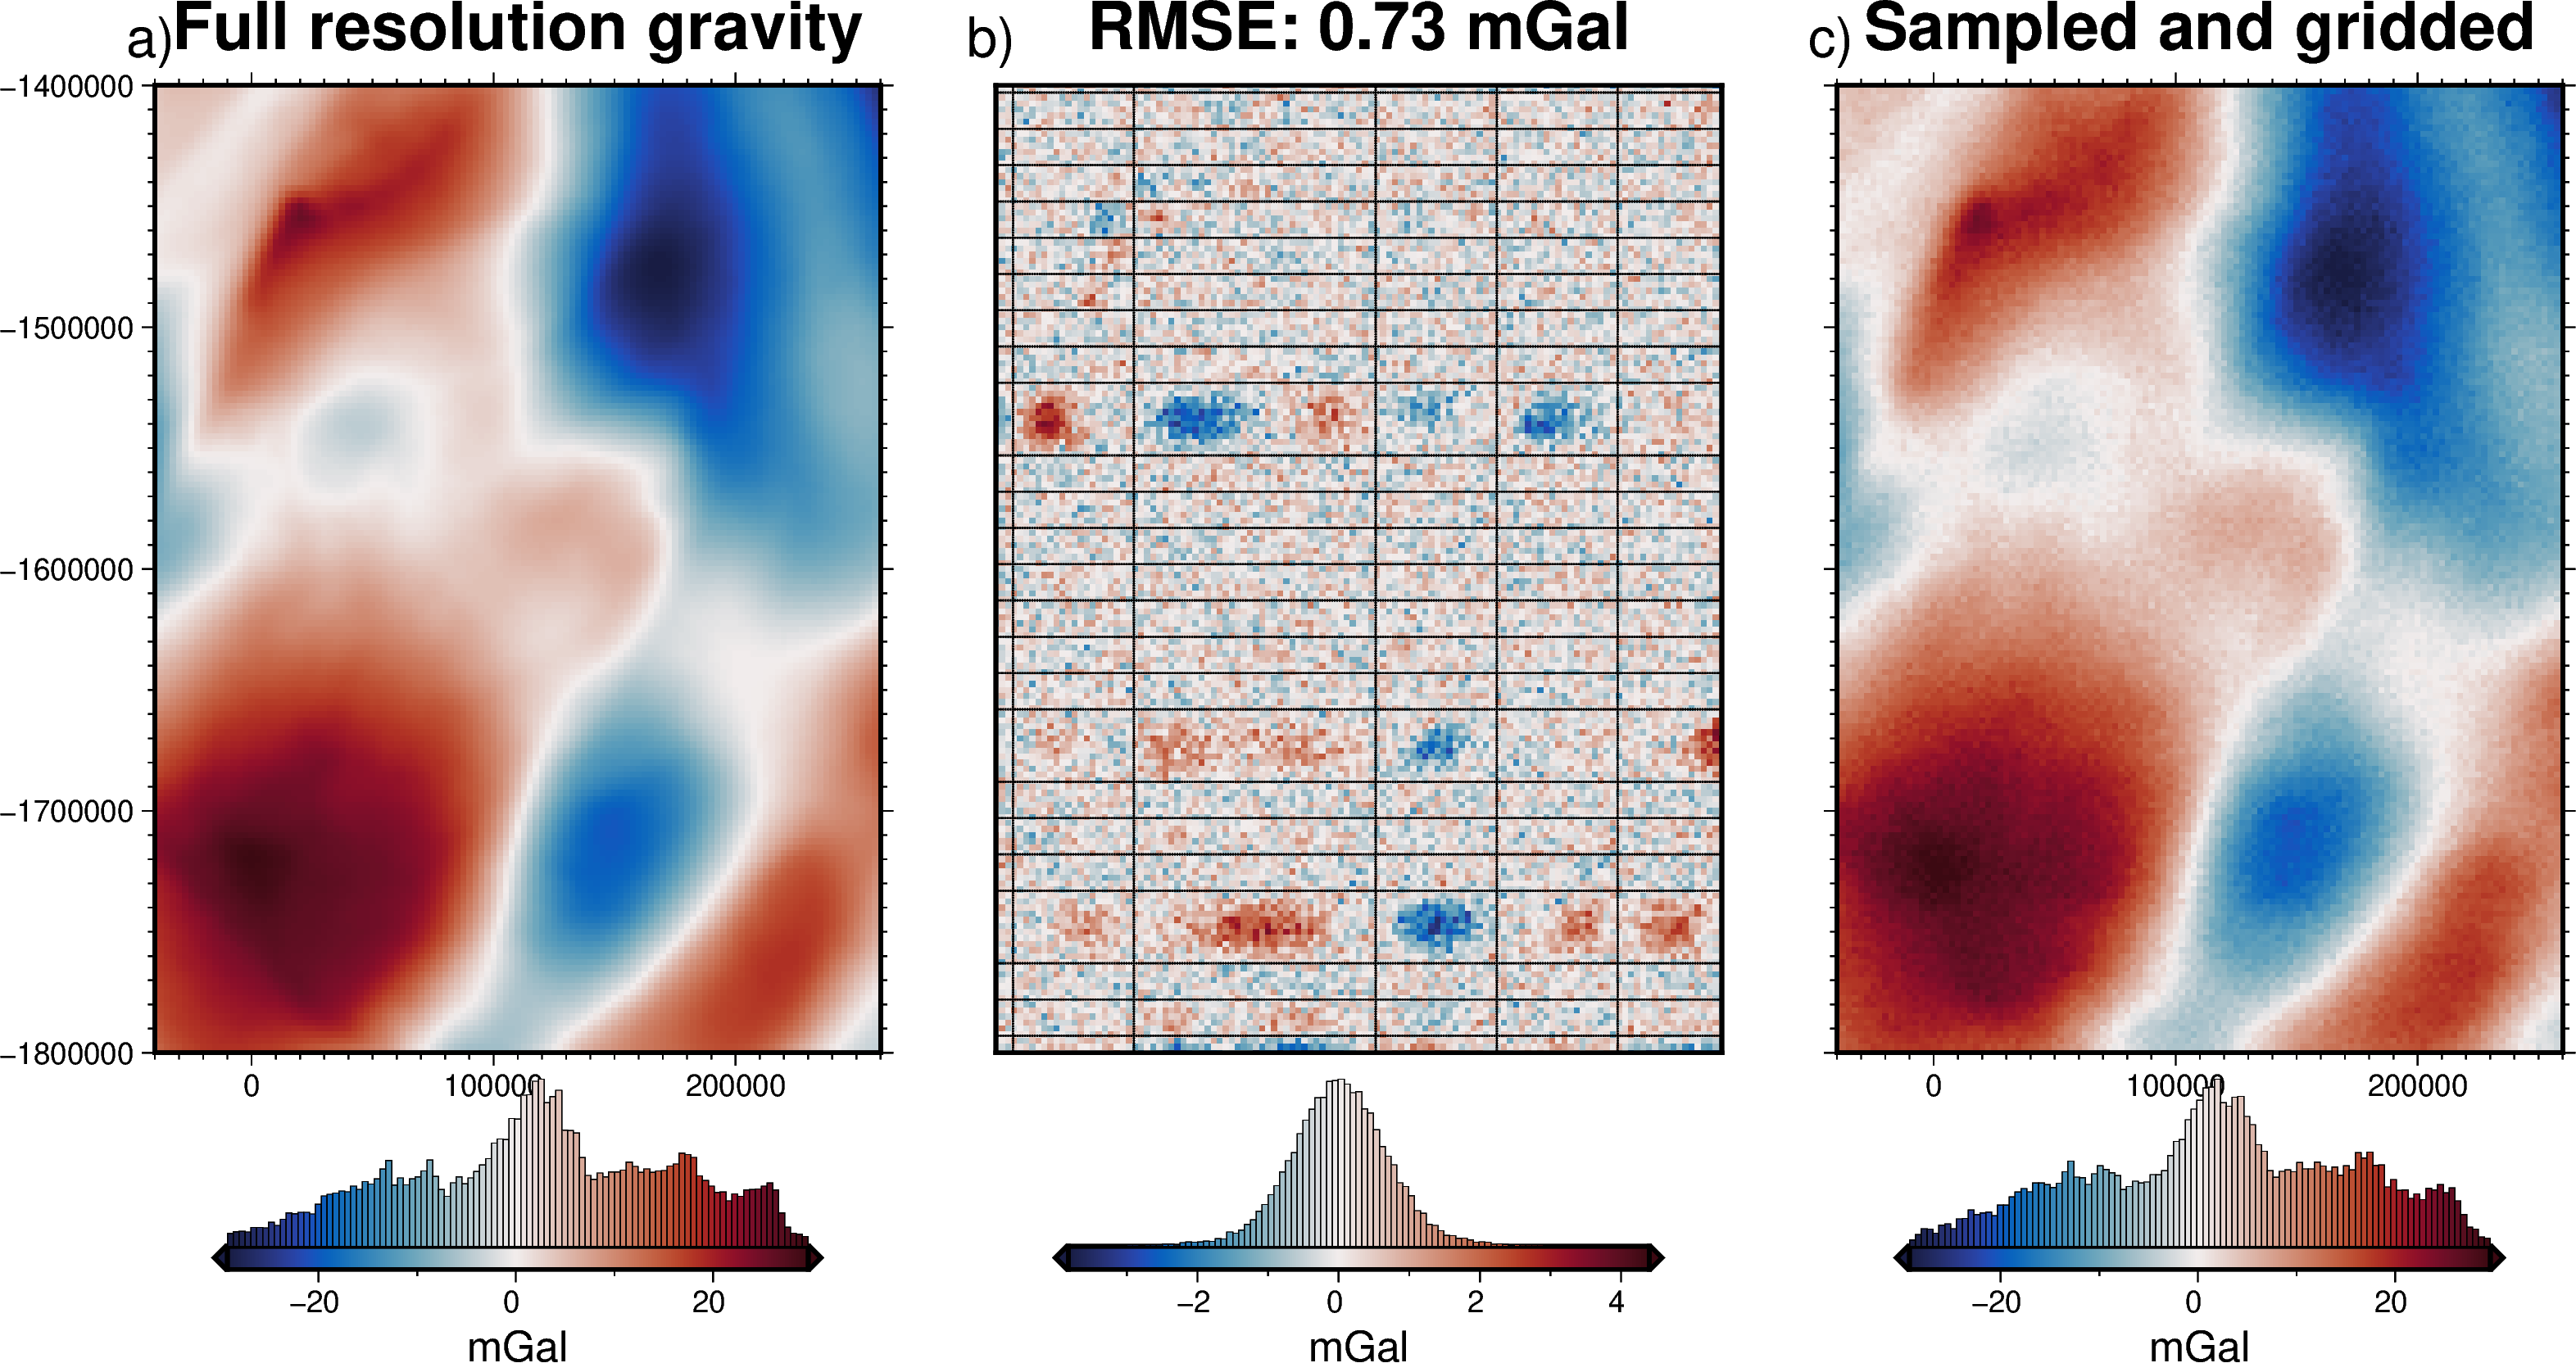
\includegraphics[width=0.8\textwidth]{figures/chp3/chp3_Ross_Sea_survey.png}
    \caption[Ross Sea synthetic airborne survey]{Ross Sea synthetic airborne survey. \textbf{a)} Full-resolution gravity data from the forward calculation of the bathymetry and basement. \textbf{b)} Difference between a and b, with black lines showing the synthetic airborne survey points. \textbf{c)} Gravity data from sampling along flight lines and re-gridded with equivalent sources.}
    \label{fig:chp3_Ross_Sea_survey}
\end{figure}

\subsection{Starting bathymetry}

The bed elevations around the borders of ice shelves are generally well-constrained. Bathymetry depths from the open ocean portion of the ice shelf border can be found through satellite altimetry or multi-beam sonar surveys. The remainder of the ice shelf border consists of grounded ice. Bed elevations beneath grounded ice can be efficiently imaged or modelled with methods such as airborne radar or mass-conservation modelling \citep{morlighemdeep2020}. Many Antarctic ice shelves also contain sparse direct measurements of bathymetry from seismic surveying. This resulting configuration for many ice shelves is generalized by a very well-constrained border with sparse constraints located within. Here, this configuration is mimicked for a hypothetical ice shelf in the Ross Sea. \\

Within the model domain, a polygon is created to represent the ice shelf border (Figure \ref{fig:chp3_Ross_Sea_starting_model}). Outside this border, constraint points are placed in each grid cell of the model ($N = 3503$, small black dots in Figure \ref{fig:chp3_Ross_Sea_starting_model}). Within the border, constraints are placed on a semi-regular grid. To represent a spatial constraint density similar to other Antarctic ice shelves\footnote{The Ross Ice Shelf has $\sim$1 constraint per 2200~km\textsuperscript{2}}, 1 constraint per 2500~km\textsuperscript{2} is used. This equates to 39 constraints. In the previous models, the true bathymetry was sampled at the constraints and the resulting values were gridded for the entire domain. Here, to represent measurement uncertainties for attaining the constraint point depths, after each point is sampled, Gaussian noise is added to the values before gridding. \\

\begin{figure}[!ht]
    \centering
    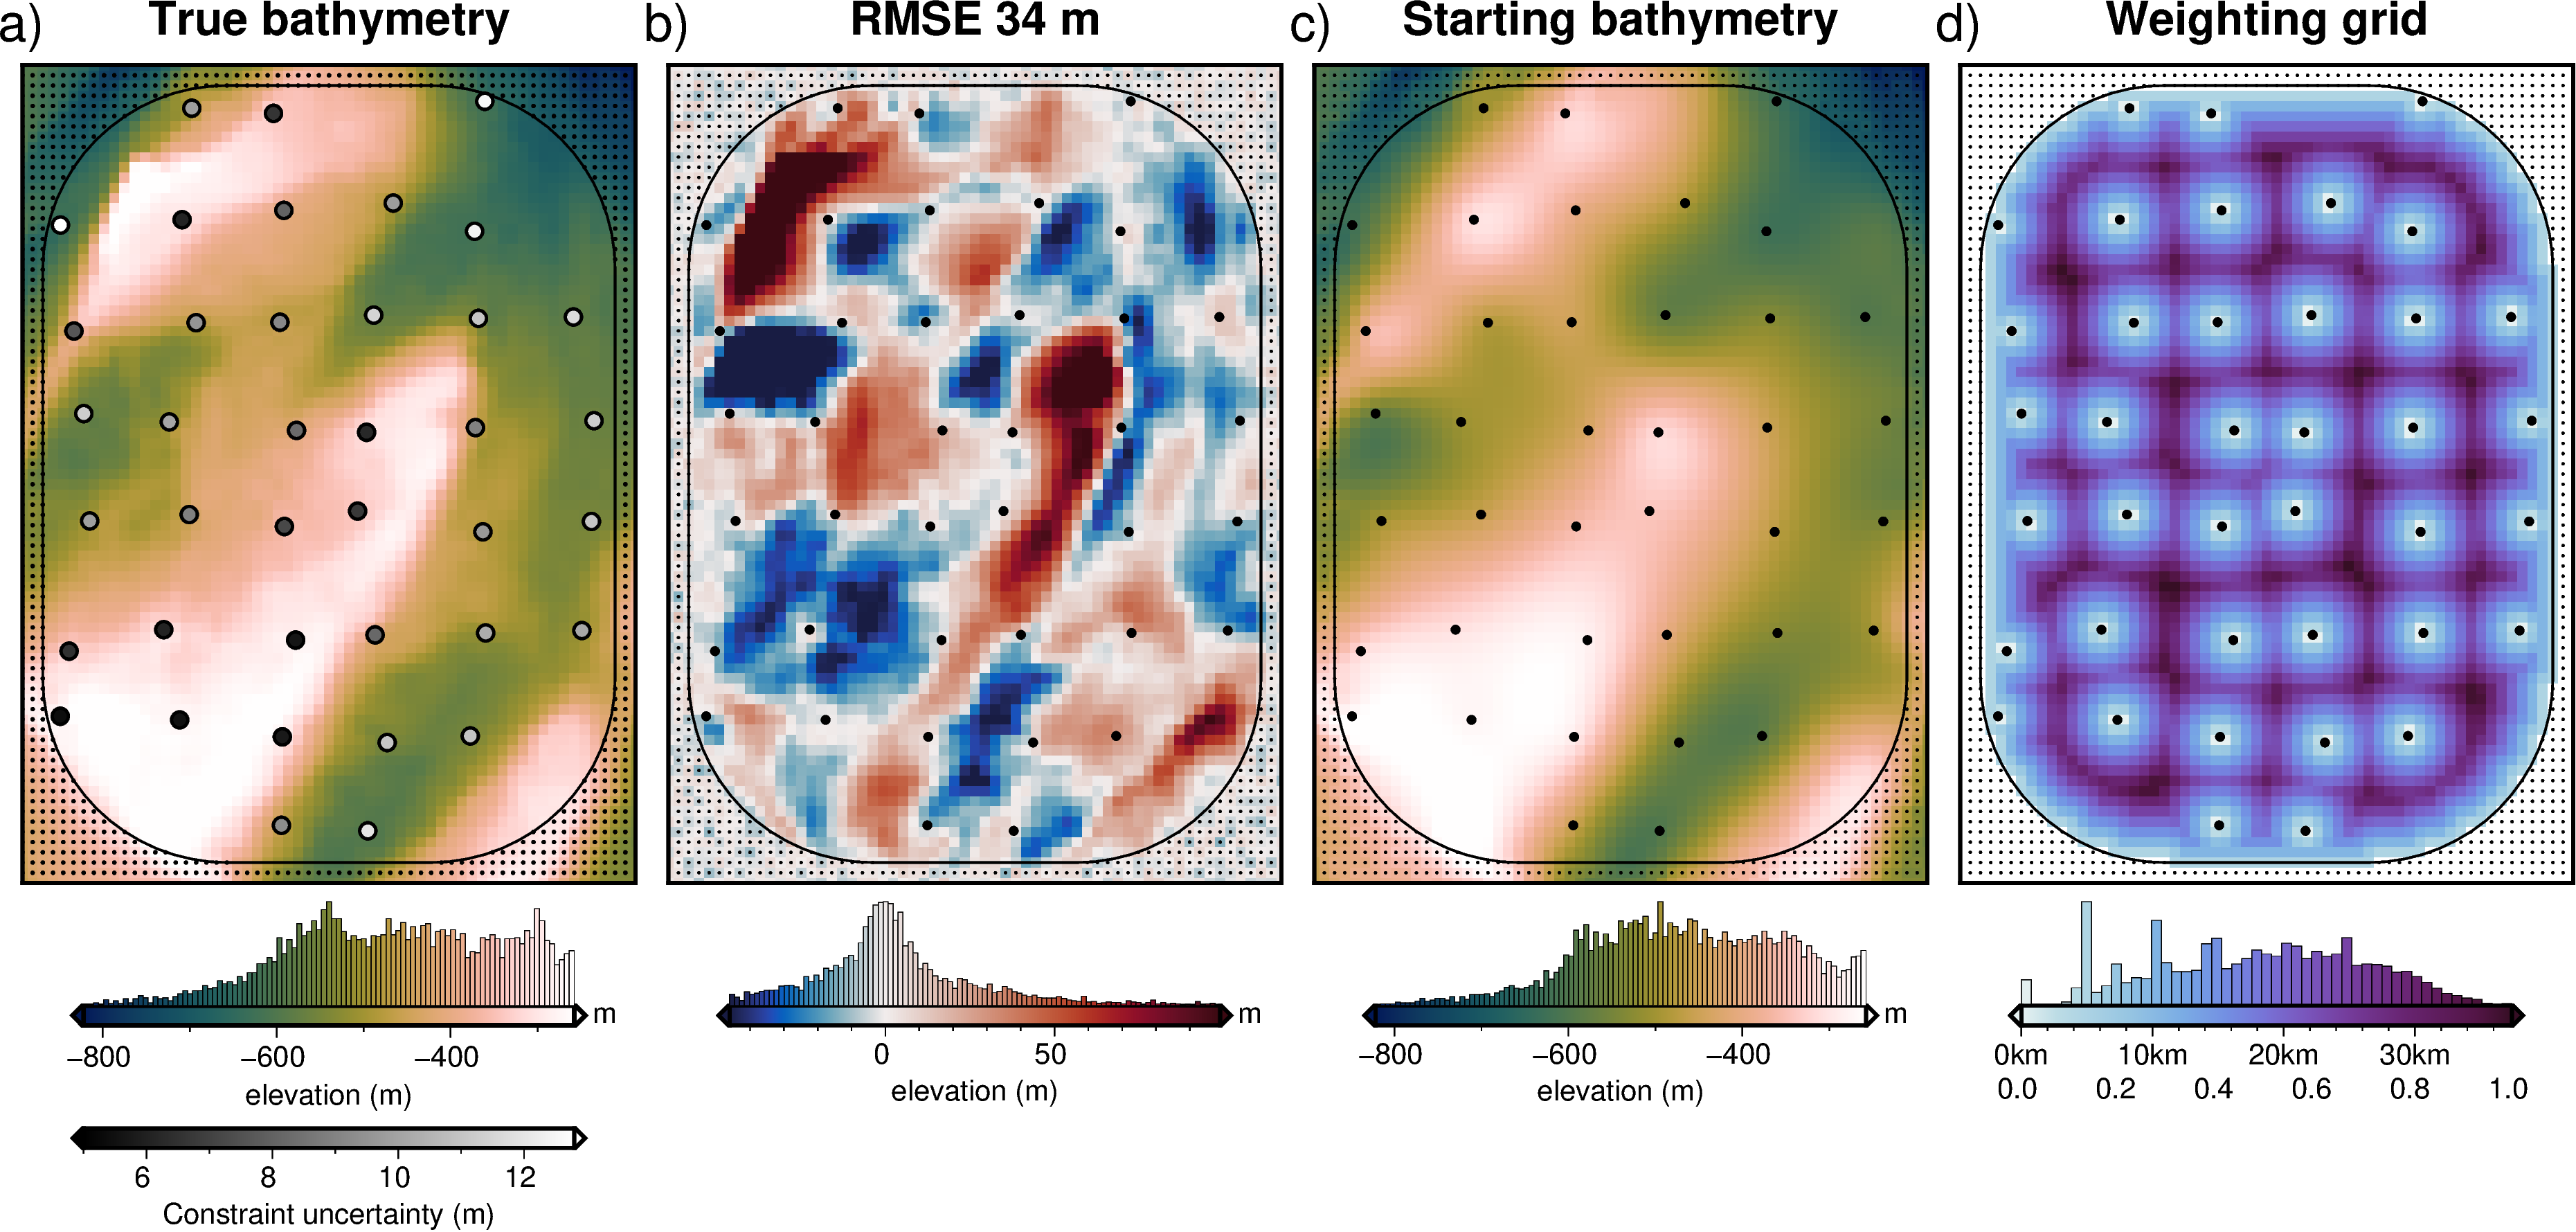
\includegraphics[width=0.95\textwidth]{figures/chp3/chp3_Ross_Sea_starting_model_semiregular.png}
    \caption[Ross Sea starting bathymetry]{Gridding of the Ross Sea starting bathymetry. \textbf{a)} True bathymetry at 5~km resolution from the IBCSO v2 compilation \citep{dorschelinternational2022}. Constraint points (coloured dots), show the uncertainty values of each point. These uncertainties were used as the standard deviations of the Gaussian function for contaminating the sampled data with noise before re-gridding. \textbf{b)} Difference between a and b, \textbf{c)} starting bathymetry from the sampling and gridding of the constraint points with added noise. \textbf{d)} Weighting grid used in the inversion. Grid colours show both the distance between each grid cell and the nearest constraint point and the weight values (0 - 1) from the normalization of these distances. Small black dots and large black dots indicate constraints outside and inside of the ice shelf border, respectively. Semi-rounded black line shows the outline of the synthetic ice shelf.}
    \label{fig:chp3_Ross_Sea_starting_model}
\end{figure}

Points outside of the ice shelf are contaminated with noise from a Gaussian distribution with a standard deviation of 5~m. This represents the well-constrained methods associated with bed observations on either grounded ice or in the open ocean. Points within the shelf are contaminated with noise based on their depth. The Gaussian distribution used has a standard deviation of 2\% of each point's depth. This simulates increasing measurement uncertainty with depth. \citet{brisbourneupdated2020} provide depth uncertainties for seismically imaged bathymetry beneath the Larsen C ice shelf, which have an average uncertainty as the percentage of depth from the surface of $\sim$2~\%. For our points, this equates to an RMS noise value of $\sim$~10 m for the ice shelf constraints. The uncertainty (the standard deviation of the Gaussian function used, not the actual value of the noise) of each point is shown in Figure \ref{fig:chp3_Ross_Sea_starting_model}a. This noise-contaminated sparse data is then gridded with a cross-validated bi-harmonic spline yielding the starting bathymetry. This interpolator takes the uncertainties of each point into account so that highly uncertain points don't introduce a bias into the interpolation \citep{uiedaverde2018}. The difference between the true and starting bathymetries had an RMS of 34~m over the whole grid, and an RMS at the constraint points of 10~m.

\subsection{Gravity misfit}

The starting bathymetry was discretized and forward modelled at the observation points with a density contrast of 1276~kg~m\textsuperscript{-1}. This forward gravity was then subtracted from the observed gravity to get the gravity misfit (Figure \ref{fig:chp3_Ross_Sea_misfit}a). Using the constraint point minimization method, the regional field was estimated with a bi-harmonic spline interpolator (Figure \ref{fig:chp3_Ross_Sea_misfit}b), which was subsequently removed, leaving the residual misfit (Figure \ref{fig:chp3_Ross_Sea_misfit}c). As in the above section, the interpolator takes the uncertainty of each constraint point into account to avoid overfitting the regional field to highly-uncertain constraint points. \\

% \begin{figure}[h]
%     \centering
%     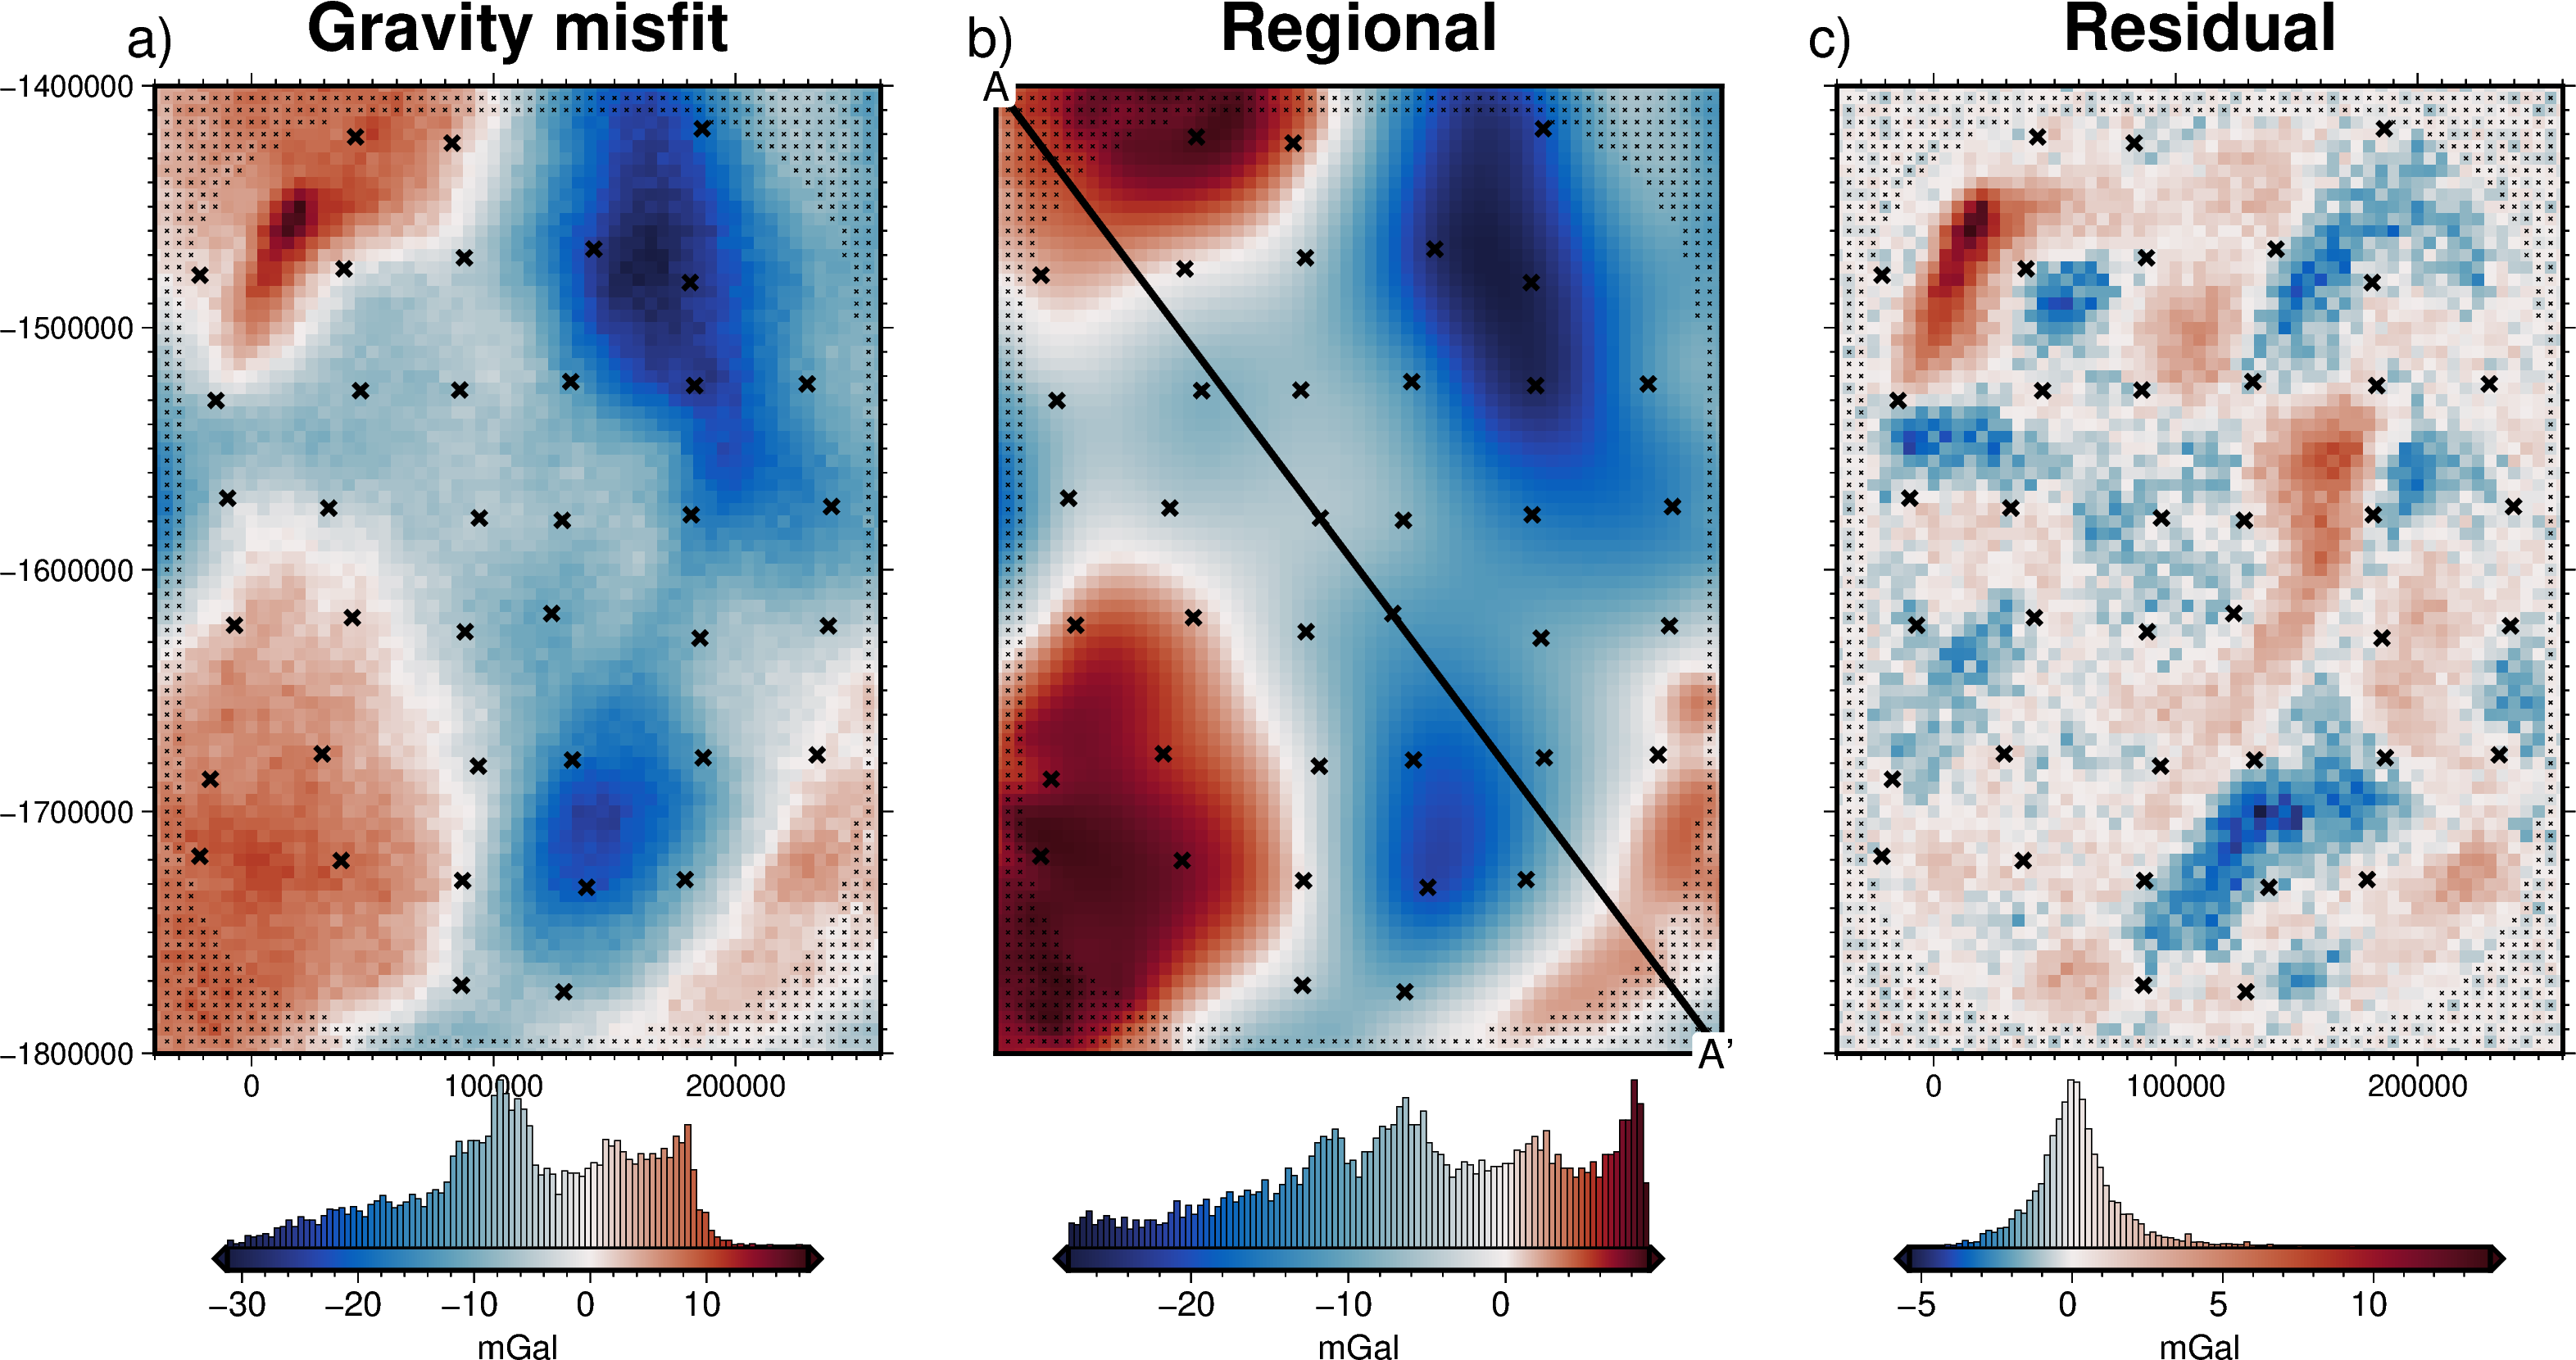
\includegraphics[width=0.95\textwidth]{figures/chp3/chp3_Ross_Sea_misfit.png}
%     \caption{Ross Sea synthetic gravity anomalies, \textbf{a)} total gravity misfit, \textbf{b)} the estimated regional component using the constraint point minimization method, and \textbf{c)}, the residual misfit, as the difference between the total misfit and the regional component. Black crosses, large and small, show constraints inside and outside the ice shelf, respectively.}
%     \label{fig:chp3_Ross_Sea_misfit}
% \end{figure}

\begin{figure}[!ht]
  \centering
    \begin{subfigure}[t]{.95\textwidth}
        \centering
        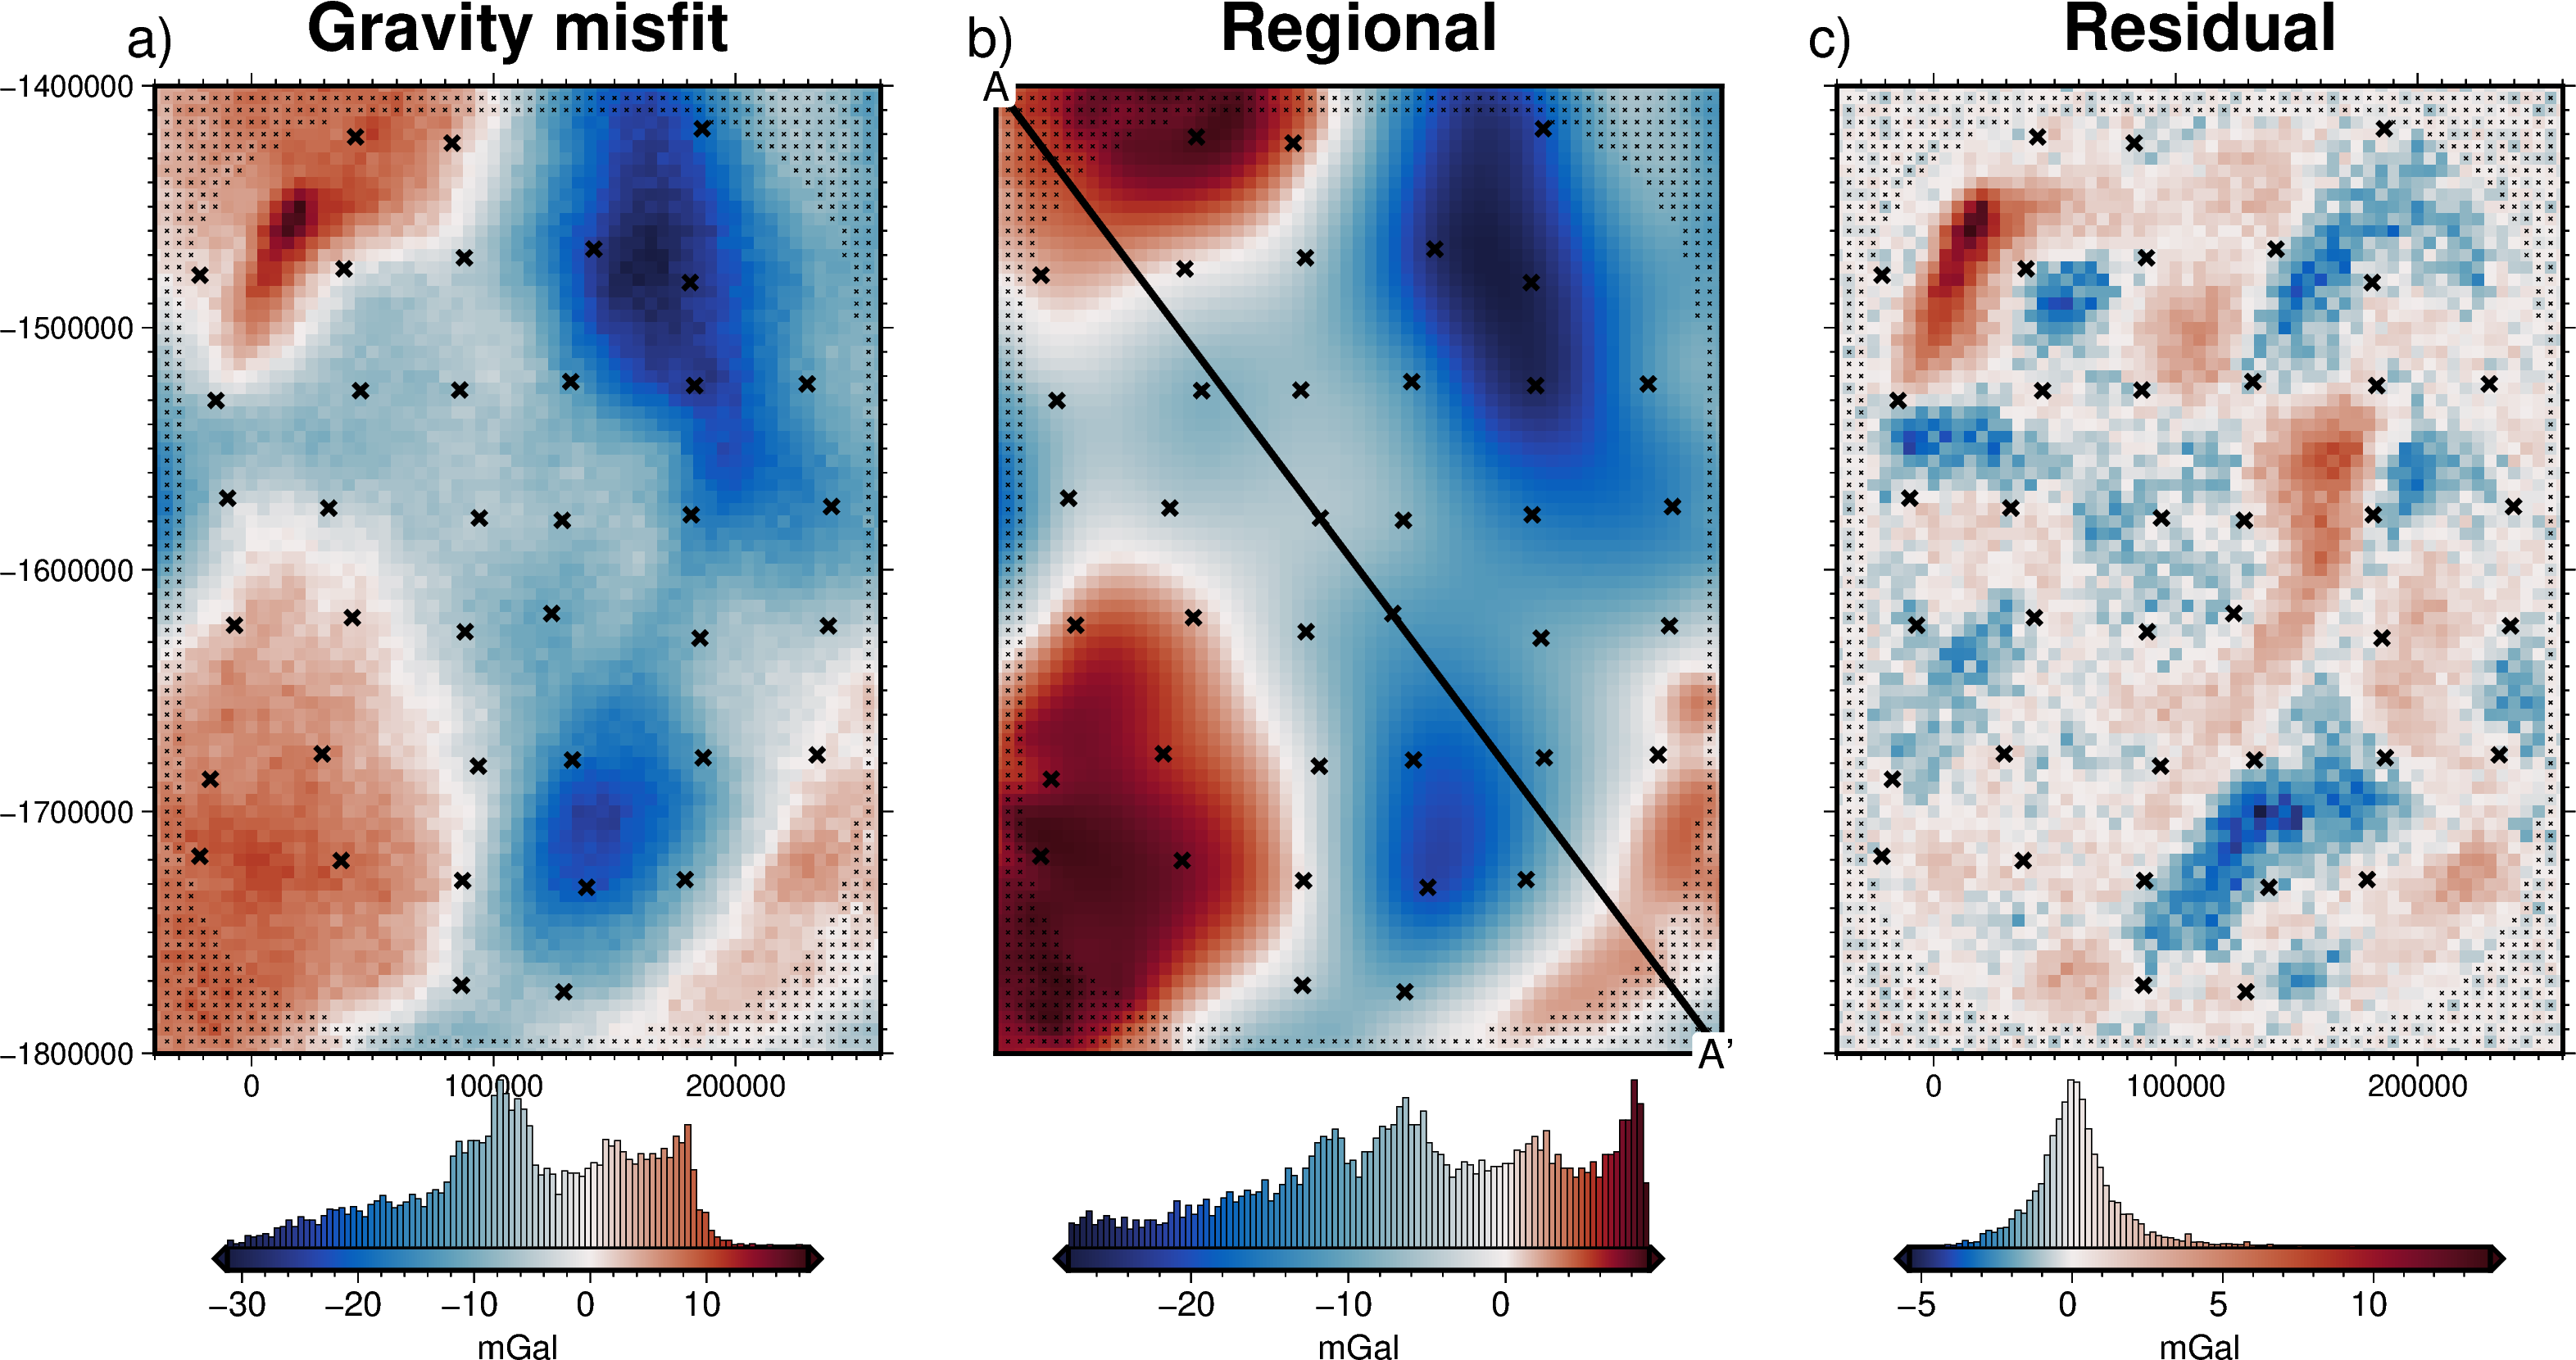
\includegraphics[width=\textwidth]{figures/chp3/chp3_Ross_Sea_misfit.png}
        % \caption{}
    \end{subfigure}
    \begin{subfigure}[t]{.95\textwidth}
        \centering
        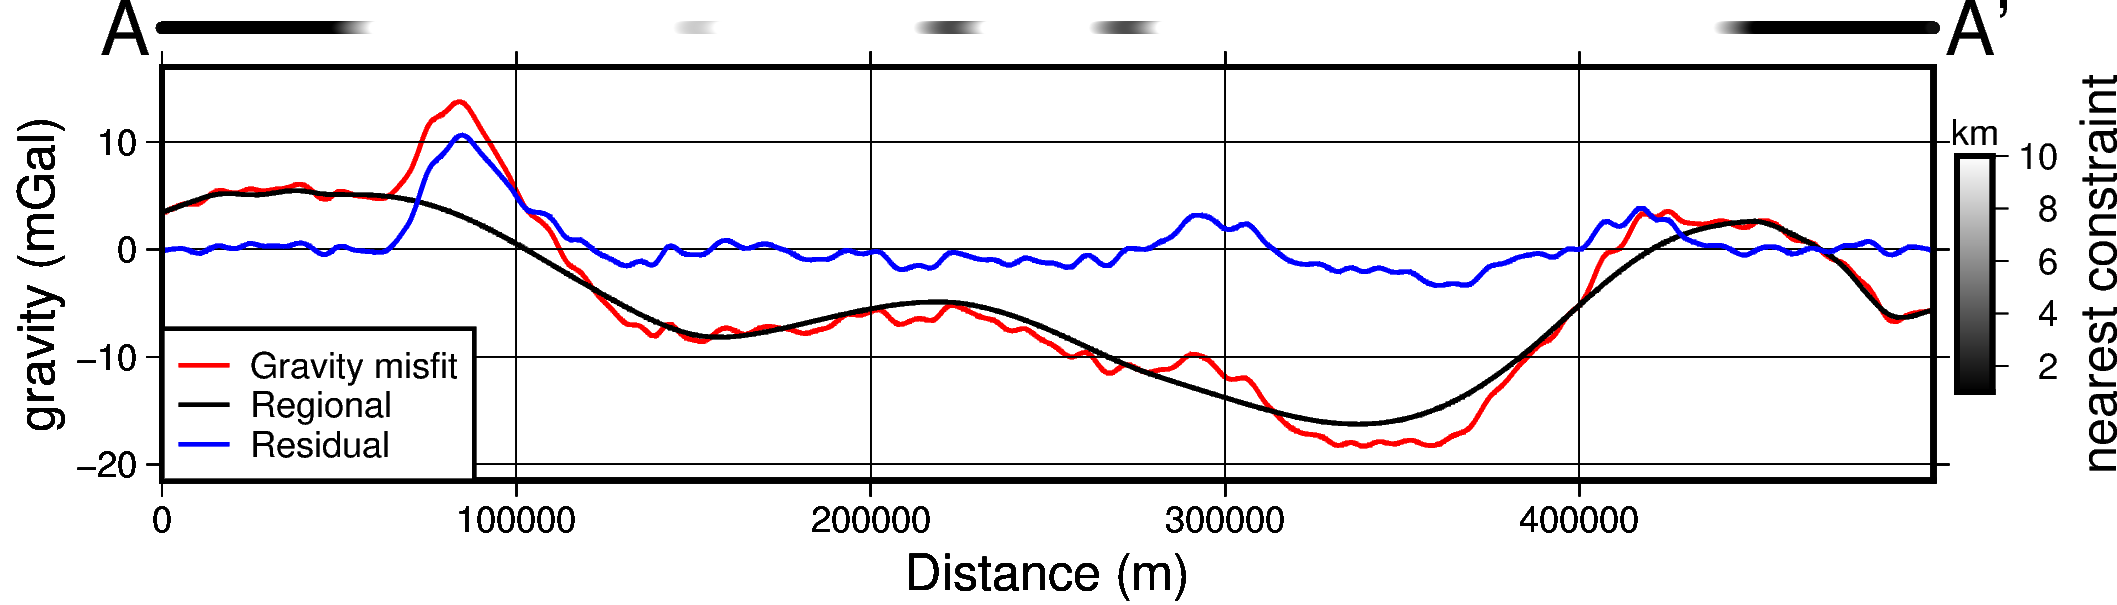
\includegraphics[width=\textwidth]{figures/chp3/chp3_Ross_Sea_misfit_profile.png}
        % \caption{}
    \end{subfigure}
  \caption[Ross Sea synthetic gravity anomalies]{Ross Sea synthetic gravity anomalies. \textbf{a)} total gravity misfit, \textbf{b)} the estimated regional component using the constraint point minimization method, and \textbf{c)}, the residual misfit, as the difference between the total misfit and the regional component. Black crosses, large and small, show constraints inside and outside the ice shelf, respectively. \textbf{Lower panel} shows profile A to A' of gravity misfit and the regional and residual components. Distance to the nearest constraint at each point along the profile shown in black to white colours at top of profile.}
    \label{fig:chp3_Ross_Sea_misfit}
\end{figure}



\subsection{Inversion}

% \begin{wrapfigure}{R}{0.4\textwidth}
%   \centering
%     \includegraphics[width=0.38\textwidth]{figures/chp3/chp3_Ross_Sea_weights.png}
%   \caption{Weighting grid calculated from the minimum distance between each grid cell and the nearest constraint point. These distance are then normalized from 0 to 1.}
%     \label{fig:chp3_Ross_Sea_weights}
% \end{wrapfigure}
% \paragraph{}
% \begin{figure}[!ht]
%     \centering
%     \includegraphics[width=0.4\textwidth]{figures/chp3/chp3_Ross_Sea_weights.png}
%     \caption{Weighting grid calculated from the minimum distance between each grid cell and the nearest constraint point. These distances are then normalized from 0 to 1.}
%     \label{fig:chp3_Ross_Sea_weights}
% \end{figure}

This residual misfit was then used in a cross-validation of 16 damping parameter values (Figure \ref{fig:chp3_Ross_Sea_CV_and_convergence}a). The inversion with the lowest cross-validation score was then chosen as the best model. During the inversions, a weighting grid was used to constrain the bathymetry at the points of known depths (Section \ref{chp3:regularization}). This grid (Figure \ref{fig:chp3_Ross_Sea_starting_model}d) is a normalized (0-1) grid of the minimum distance between each grid cell and the nearest constraint point. The inversion result and the difference from the true bathymetry are shown in Figure \ref{fig:chp3_Ross_Sea_results}. The inversion had an RMS difference with the true Ross Sea bathymetry of 21~m and an RMS at the constraints of $<$~1~m. The inversion converged in 12 seconds at 15 iterations and had a final residual misfit of 0.43~mGal (Figure \ref{fig:chp3_Ross_Sea_CV_and_convergence}b).  \\ 

\begin{figure}[!ht]
  \centering
    \begin{subfigure}[t]{.45\textwidth}
        \centering
        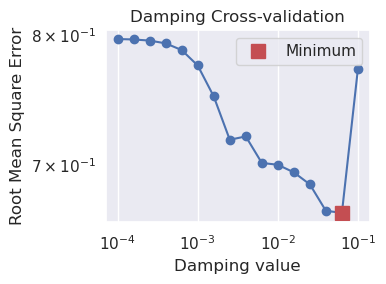
\includegraphics[width=\textwidth]{figures/chp3/chp3_Ross_Sea_CV.png}
        \caption{}
    \end{subfigure}
    \begin{subfigure}[t]{.45\textwidth}
        \centering
        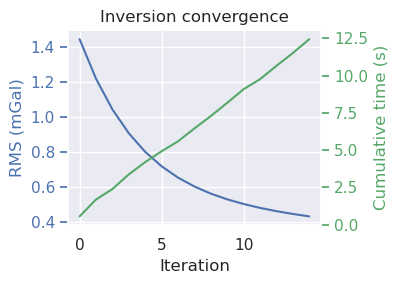
\includegraphics[width=\textwidth]{figures/chp3/chp3_Ross_Sea_convergence.png}
        \caption{}
    \end{subfigure}
  \caption[Ross Sea inversion, CV and convergence]{\textbf{a)} Cross-validation curve showing the optimal damping parameter (red square). \textbf{b)} Convergence of the inversion misfit. Blue line (left y-axis) shows the RMS of the residual misfit at each iteration of the inversion. Green line (right y-axis) shows the cumulative time to complete the inversion. 
  }
    \label{fig:chp3_Ross_Sea_CV_and_convergence}
\end{figure}

\begin{figure}[!ht]
  \centering
    \begin{subfigure}[t]{.9\textwidth}
        \centering
        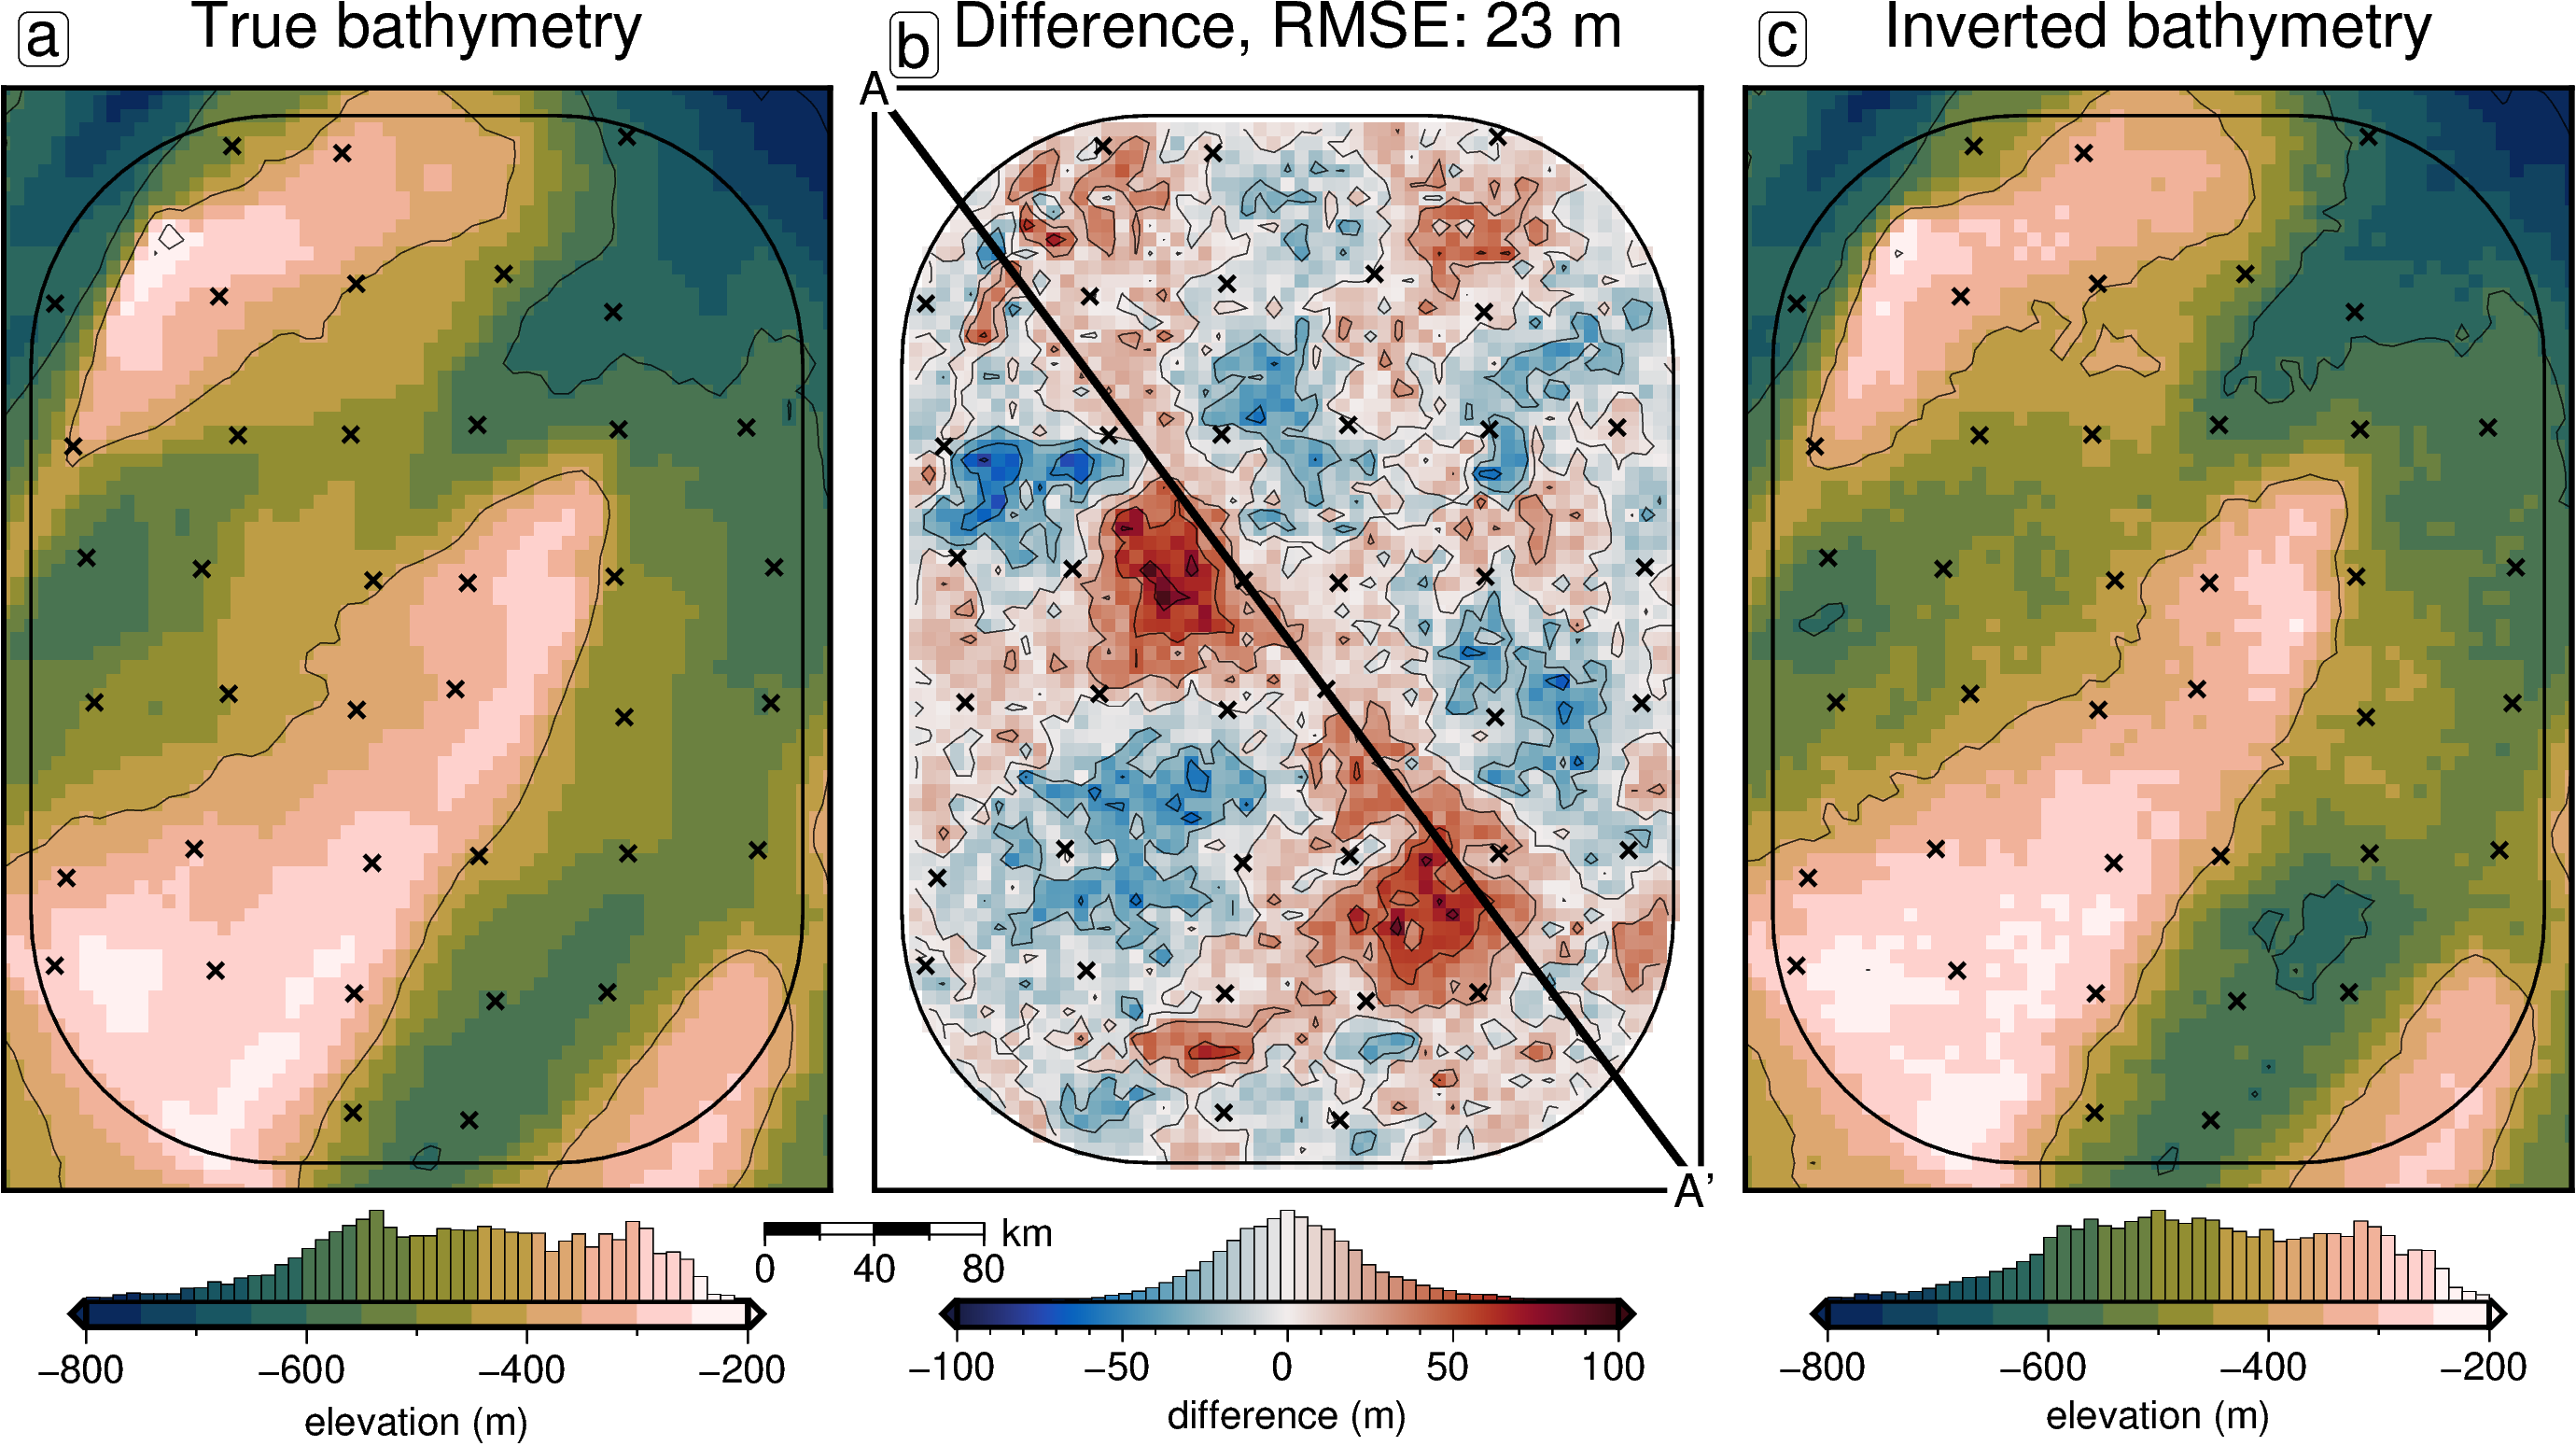
\includegraphics[width=\textwidth]{figures/chp3/chp3_Ross_Sea_results.png}
        % \caption{}
    \end{subfigure}
    \begin{subfigure}[t]{.7\textwidth}
        % \addtocounter{subfigure}{3}
        \centering
        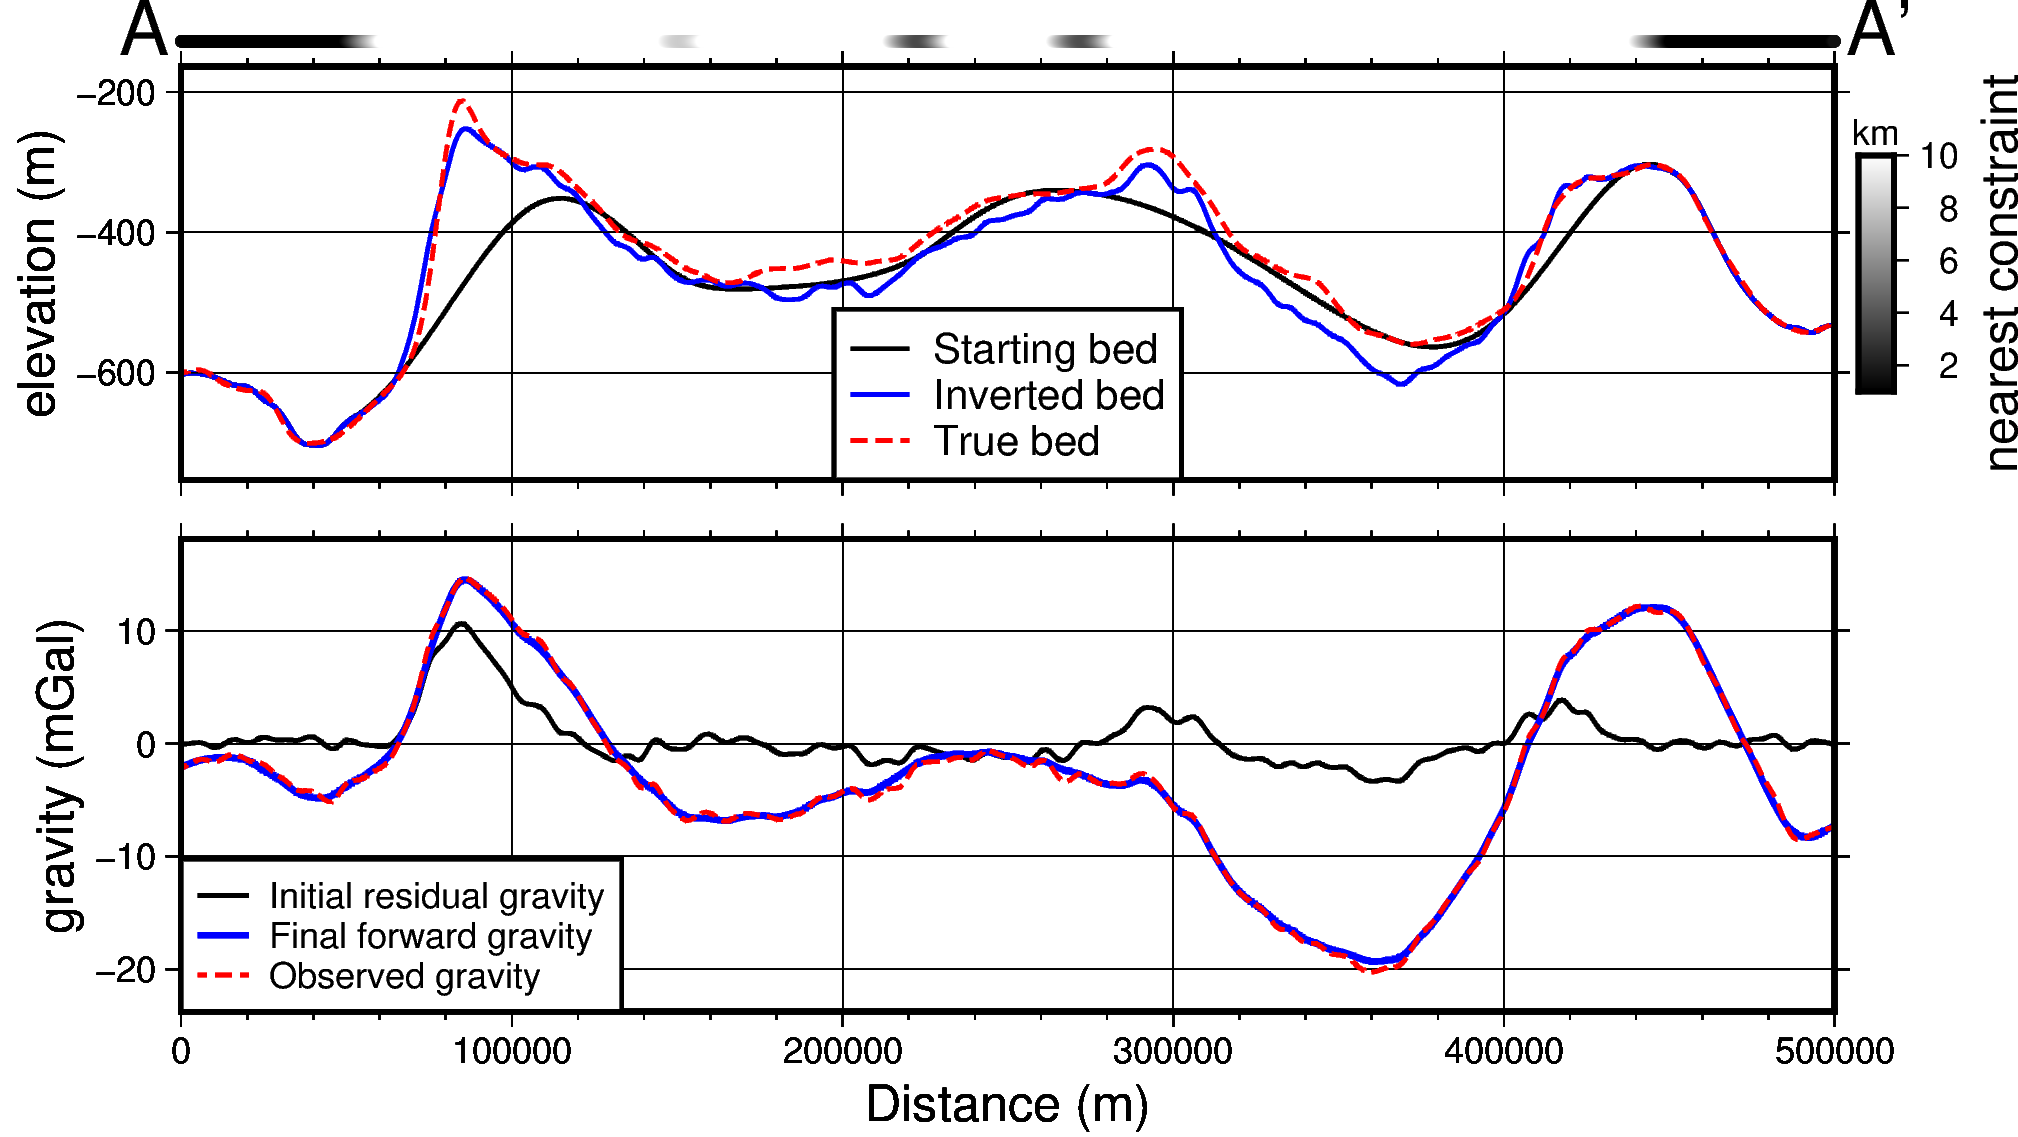
\includegraphics[width=\textwidth]{figures/chp3/chp3_Ross_Sea_profile.png}
        % \caption{}
    \end{subfigure}
  \caption[Ross Sea inversion results]{Ross Sea synthetic model inversion results. \textbf{a)} True bathymetry, \textbf{b)} difference between a and c, and \textbf{c)} final inverted bathymetry. Black crosses are constraint points. The RMS difference with the true bathymetry at these constraints is $<$~1~m. \textbf{Lower panel)} Profile from A to A'. The top panel contains topographic profiles of the starting, inverted, and true bathymetries. The bottom panel contains gravity anomaly profiles. Distance to the nearest constraint at each point along the profile shown in black to white colours at top of profile.}
    \label{fig:chp3_Ross_Sea_results}
\end{figure}

% \begin{figure}[!ht]
%   \centering
%     \begin{subfigure}[t]{.5\textwidth}
%         \centering
%         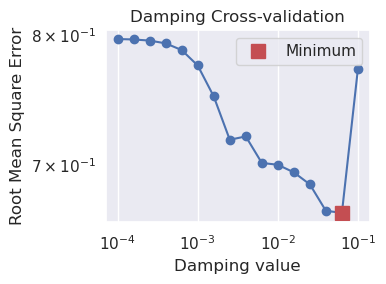
\includegraphics[width=\textwidth]{figures/chp3/chp3_Ross_Sea_CV.png}
%         \caption{}
%     \end{subfigure}
%     \begin{subfigure}[t]{.8\textwidth}
%         \centering
%         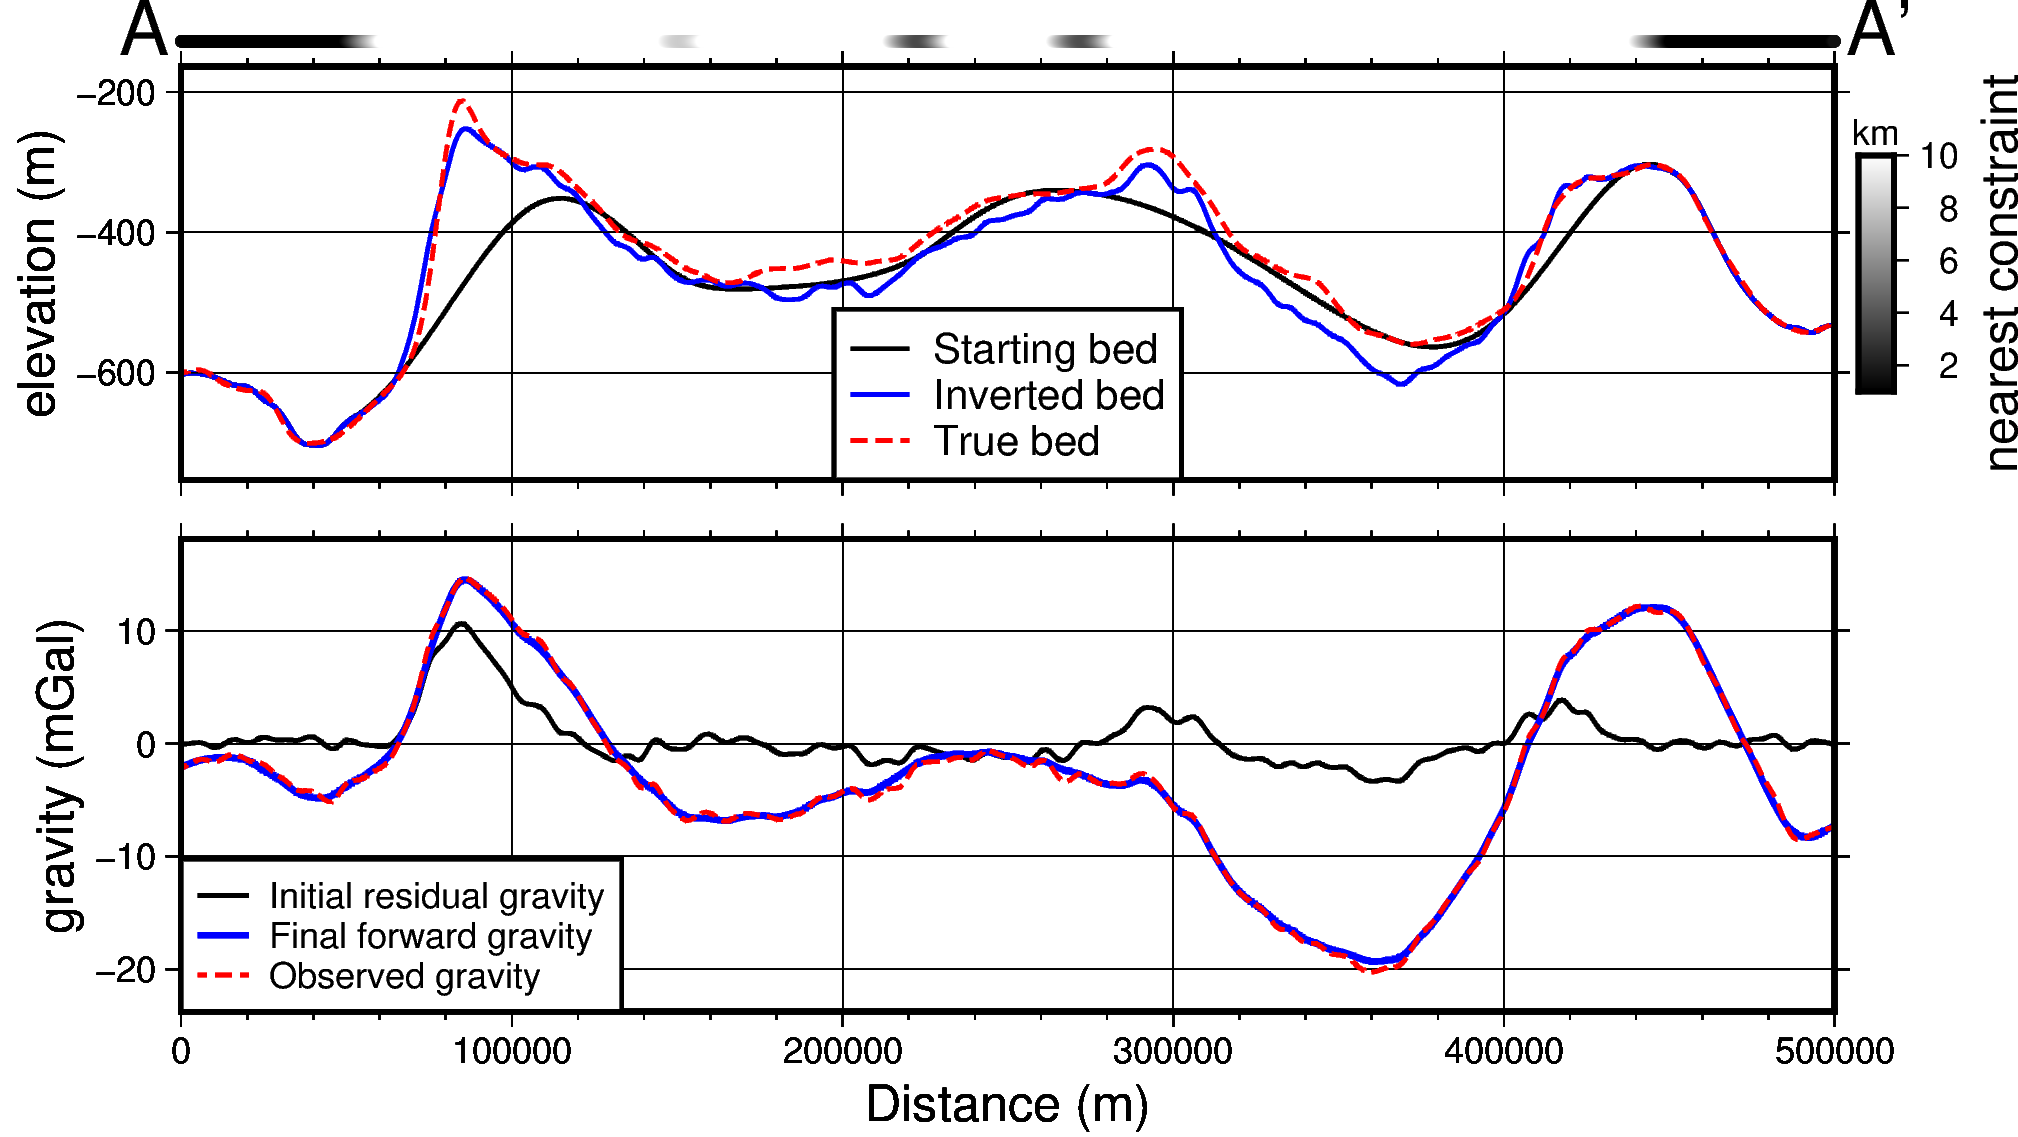
\includegraphics[width=\textwidth]{figures/chp3/chp3_Ross_Sea_profile.png}
%         \caption{}
%     \end{subfigure}
%   \caption{Cross-validation and profiles for the Ross Sea synthetic inversion with a regional component removed. \textbf{a)} Cross-validation curve showing the optimal damping parameter (red square). \textbf{b)} 2D profile of the inversion results. The top panel shows profile location and constraint points (black crosses). The middle panel contains topographic profiles of the starting, inverted, and true bathymetries. The bottom panel contains gravity anomaly profiles.}
%     \label{fig:chp3_Ross_Sea_CV_and_profile}
% \end{figure}

% \begin{figure}[!ht]
%     \centering
%     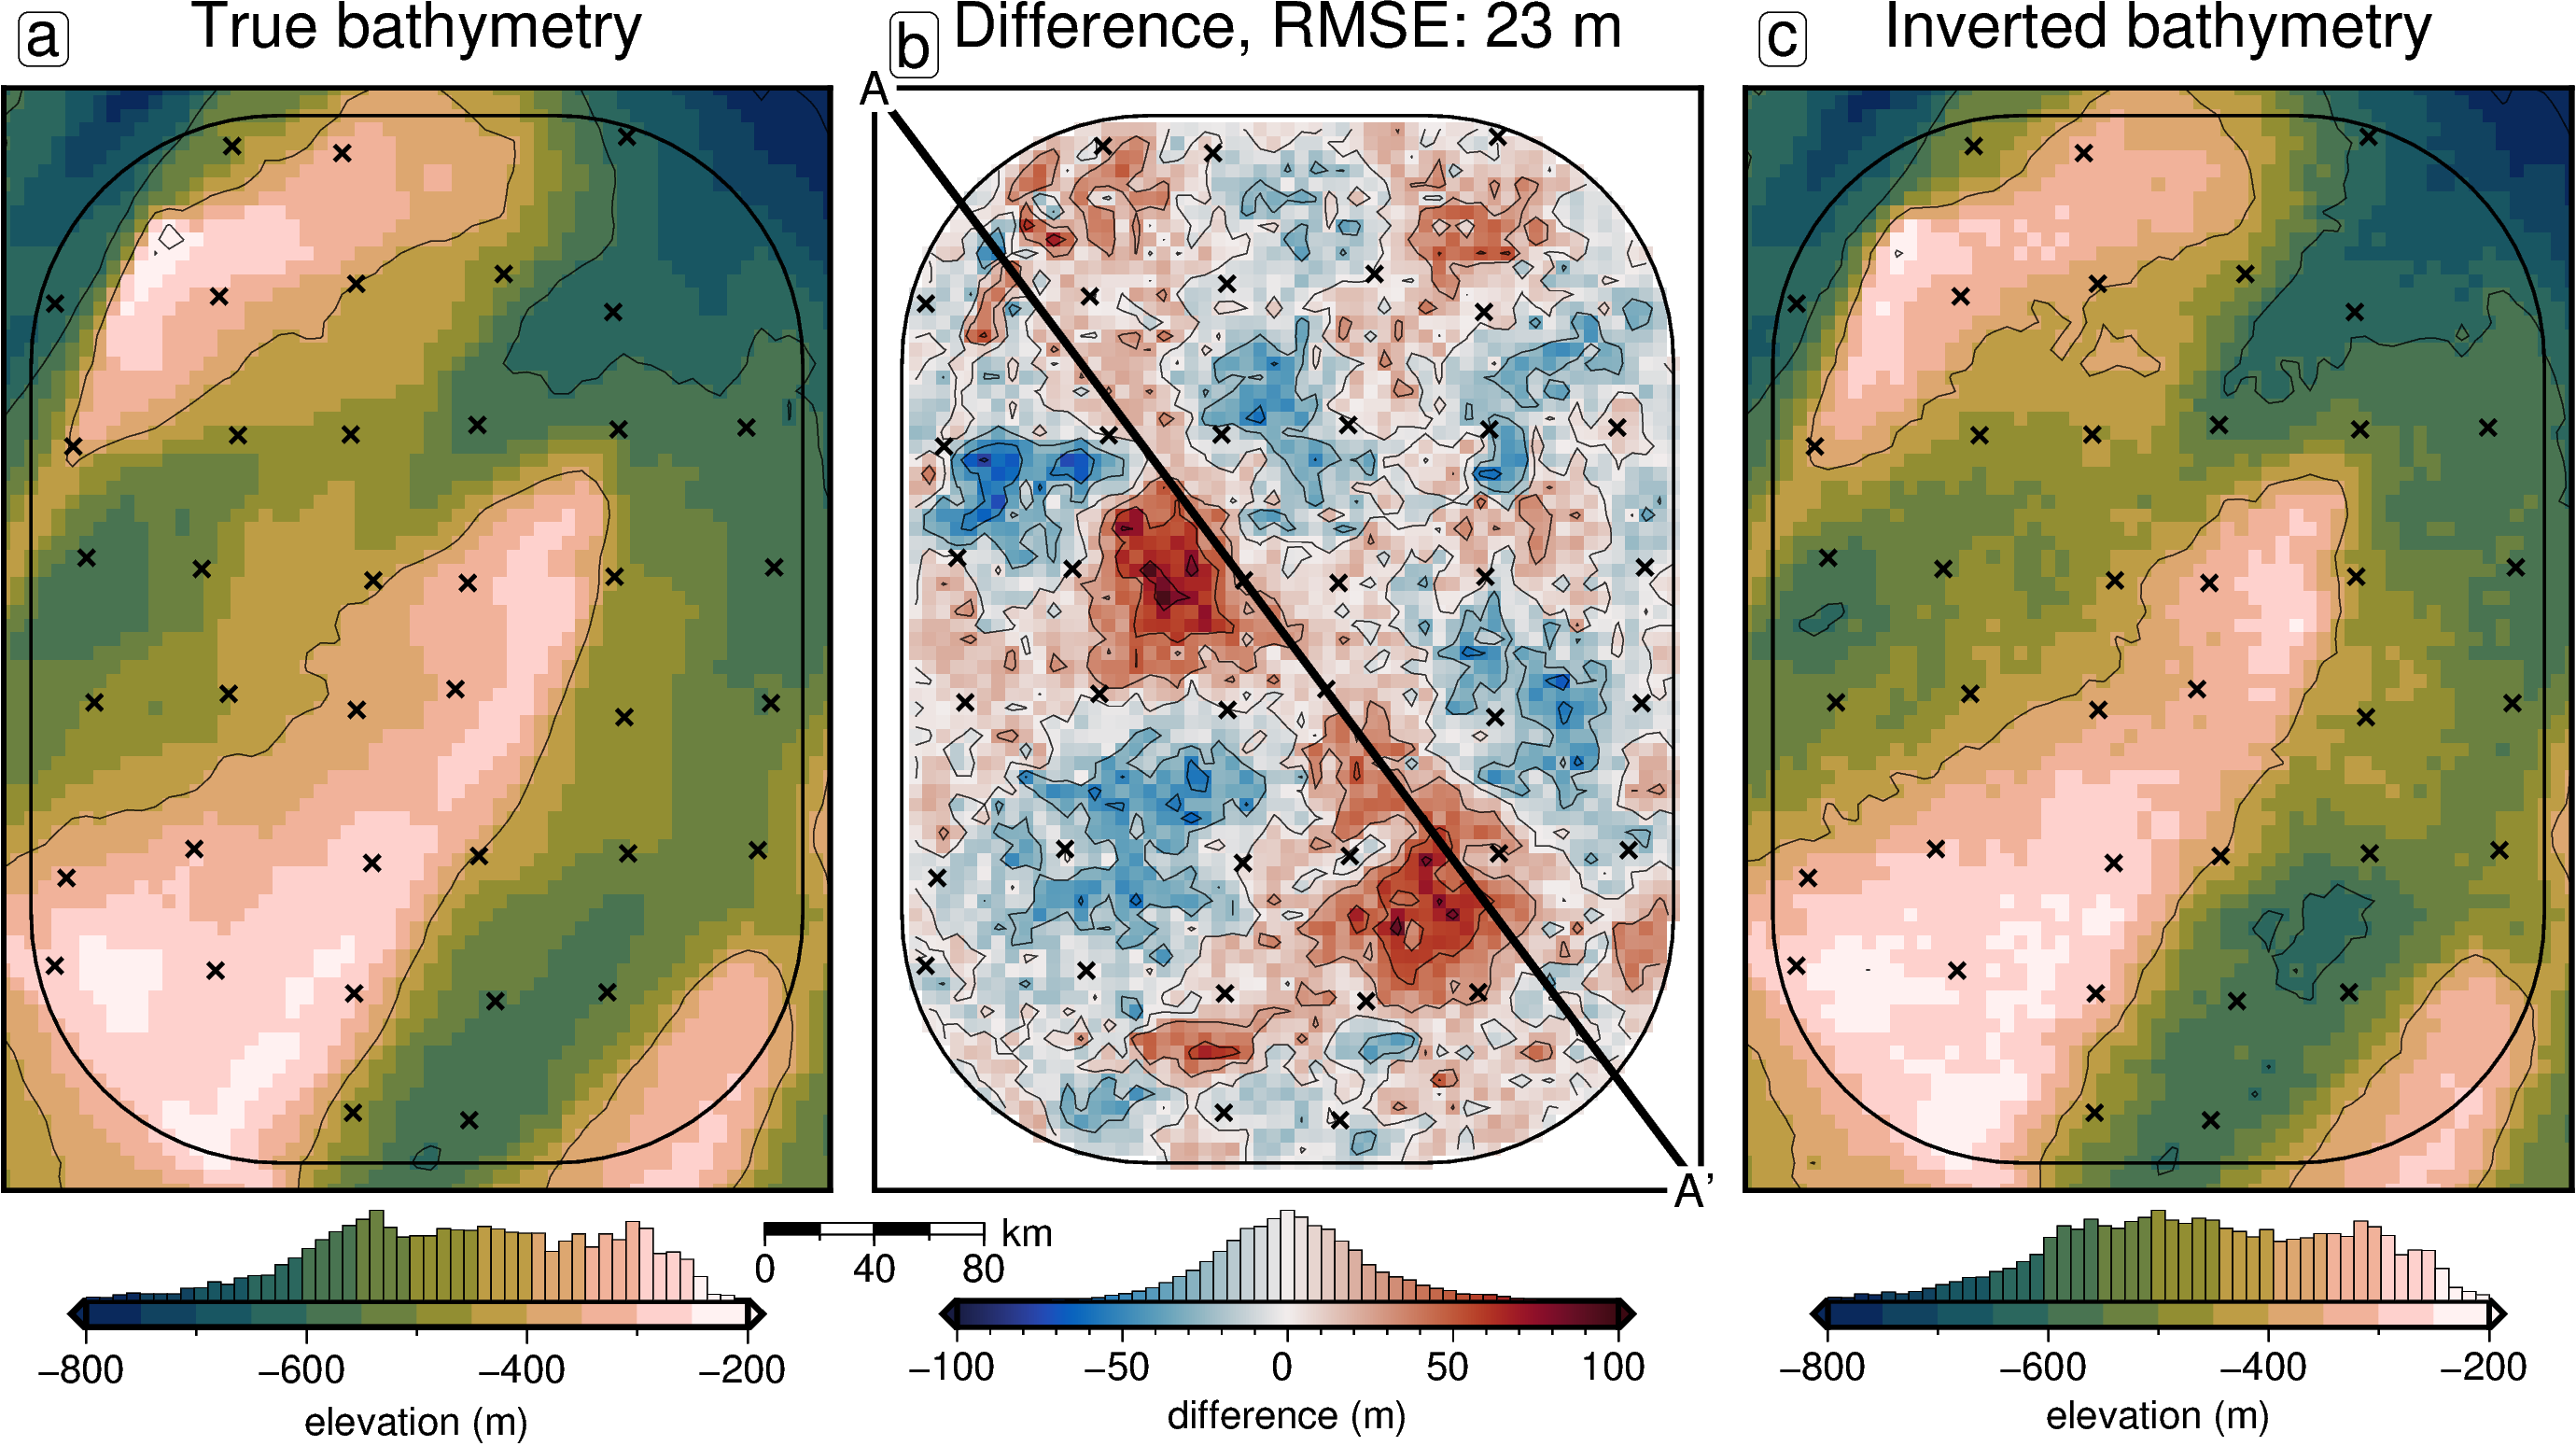
\includegraphics[width=0.95\textwidth]{figures/chp3/chp3_Ross_Sea_results.png}
%     \caption{Ross Sea synthetic model inversion results. \textbf{a)} True bathymetry, \textbf{b)} difference between a and c, and \textbf{c)} final inverted bathymetry. Black crosses are constraint points. The RMS difference with the true bathymetry at these constraints is $<$ 1 m.}
%     \label{fig:chp3_Ross_Sea_results}
% \end{figure}

\subsection{Uncertainty analysis} \label{chp3:monte_carlo}

Since the true Ross Sea bathymetry for this inversion is known, a direct measurement of the spatial uncertainty of the resulting bathymetry is simple to calculate (Figure \ref{fig:chp3_Ross_Sea_results}b). This spatial uncertainty is useful to provide alongside the bathymetry results. It informs ocean modellers where results can be confidently interpreted and highlights regions to focus future data collection. Here, a method of uncertainty analysis for this inversion is proposed, and the resulting uncertainty is compared to the inversion error to get a sense of the accuracy of our calculation of uncertainty. This uncertainty analysis is accomplished with Monte Carlo simulations \citep{jansenmonte1994, heltonsurvey2006}. \\

Here, 20 inversions are run with the same damping parameter cross-validation as conducted previously. For each inversion, the input parameters are sampled from distributions of their possible values. These prior distributions represent all plausible parameter values and thus the resulting inverted bathymetries should cover the range of plausible inversion outcomes. For each grid cell, the weighted standard deviation of the 20 inverted bathymetry values of that grid cell was calculated. The weighting came from the inverse square of each inversion's RMS difference between the inverted grid values and the constraint point depths. This reduces the bias from inversions with large misfits to the actual constraint points \citep{schnaidtbootstrap2015}. Chapter \ref{ch:4} Section \ref{chp4_uncertainty_method} contains a detailed description of this uncertainty analysis methodology. \\


% \sigma^*_j = \left[
% \frac
% {\sum_{i=1}^{N}w_i (z_{ij}-\bar{z^*_{ij}})^2}
% {\sum_{i=1}^{N}w_i}  
% \right]^\frac{1}{2},
% \\
% \text{where $z_{ij}$ is the $j^{th}$ cell of the $i^{th}$ inverted bathymetry}

The parameters included in the Monte Carlo sampling are:
\begin{enumerate}
    \item the observed gravity data, sampled from a normal distribution with a mean equal to the observed values and a standard deviation of 0.6~mGal (2\% of the maximum absolute value).
    \item the constraint point depths, sampled from a uniform distribution with a centre as the measured point depth and bounds of $\pm$5~m for the points outside the ice shelf, and $\pm$2\% depth for points within the shelf.
    \item the bathymetry density contrast. This is defined as the difference between the densities of water and sediment. The mean value was taken to be 1276~kg~m\textsuperscript{-1} (2300~-~1024~kg~m\textsuperscript{-1}). A standard deviation of 400~kg~m\textsuperscript{-1} was used.
\end{enumerate} 

\begin{figure}[!ht]
  \centering
    \begin{subfigure}[t]{.9\textwidth}
        \centering
        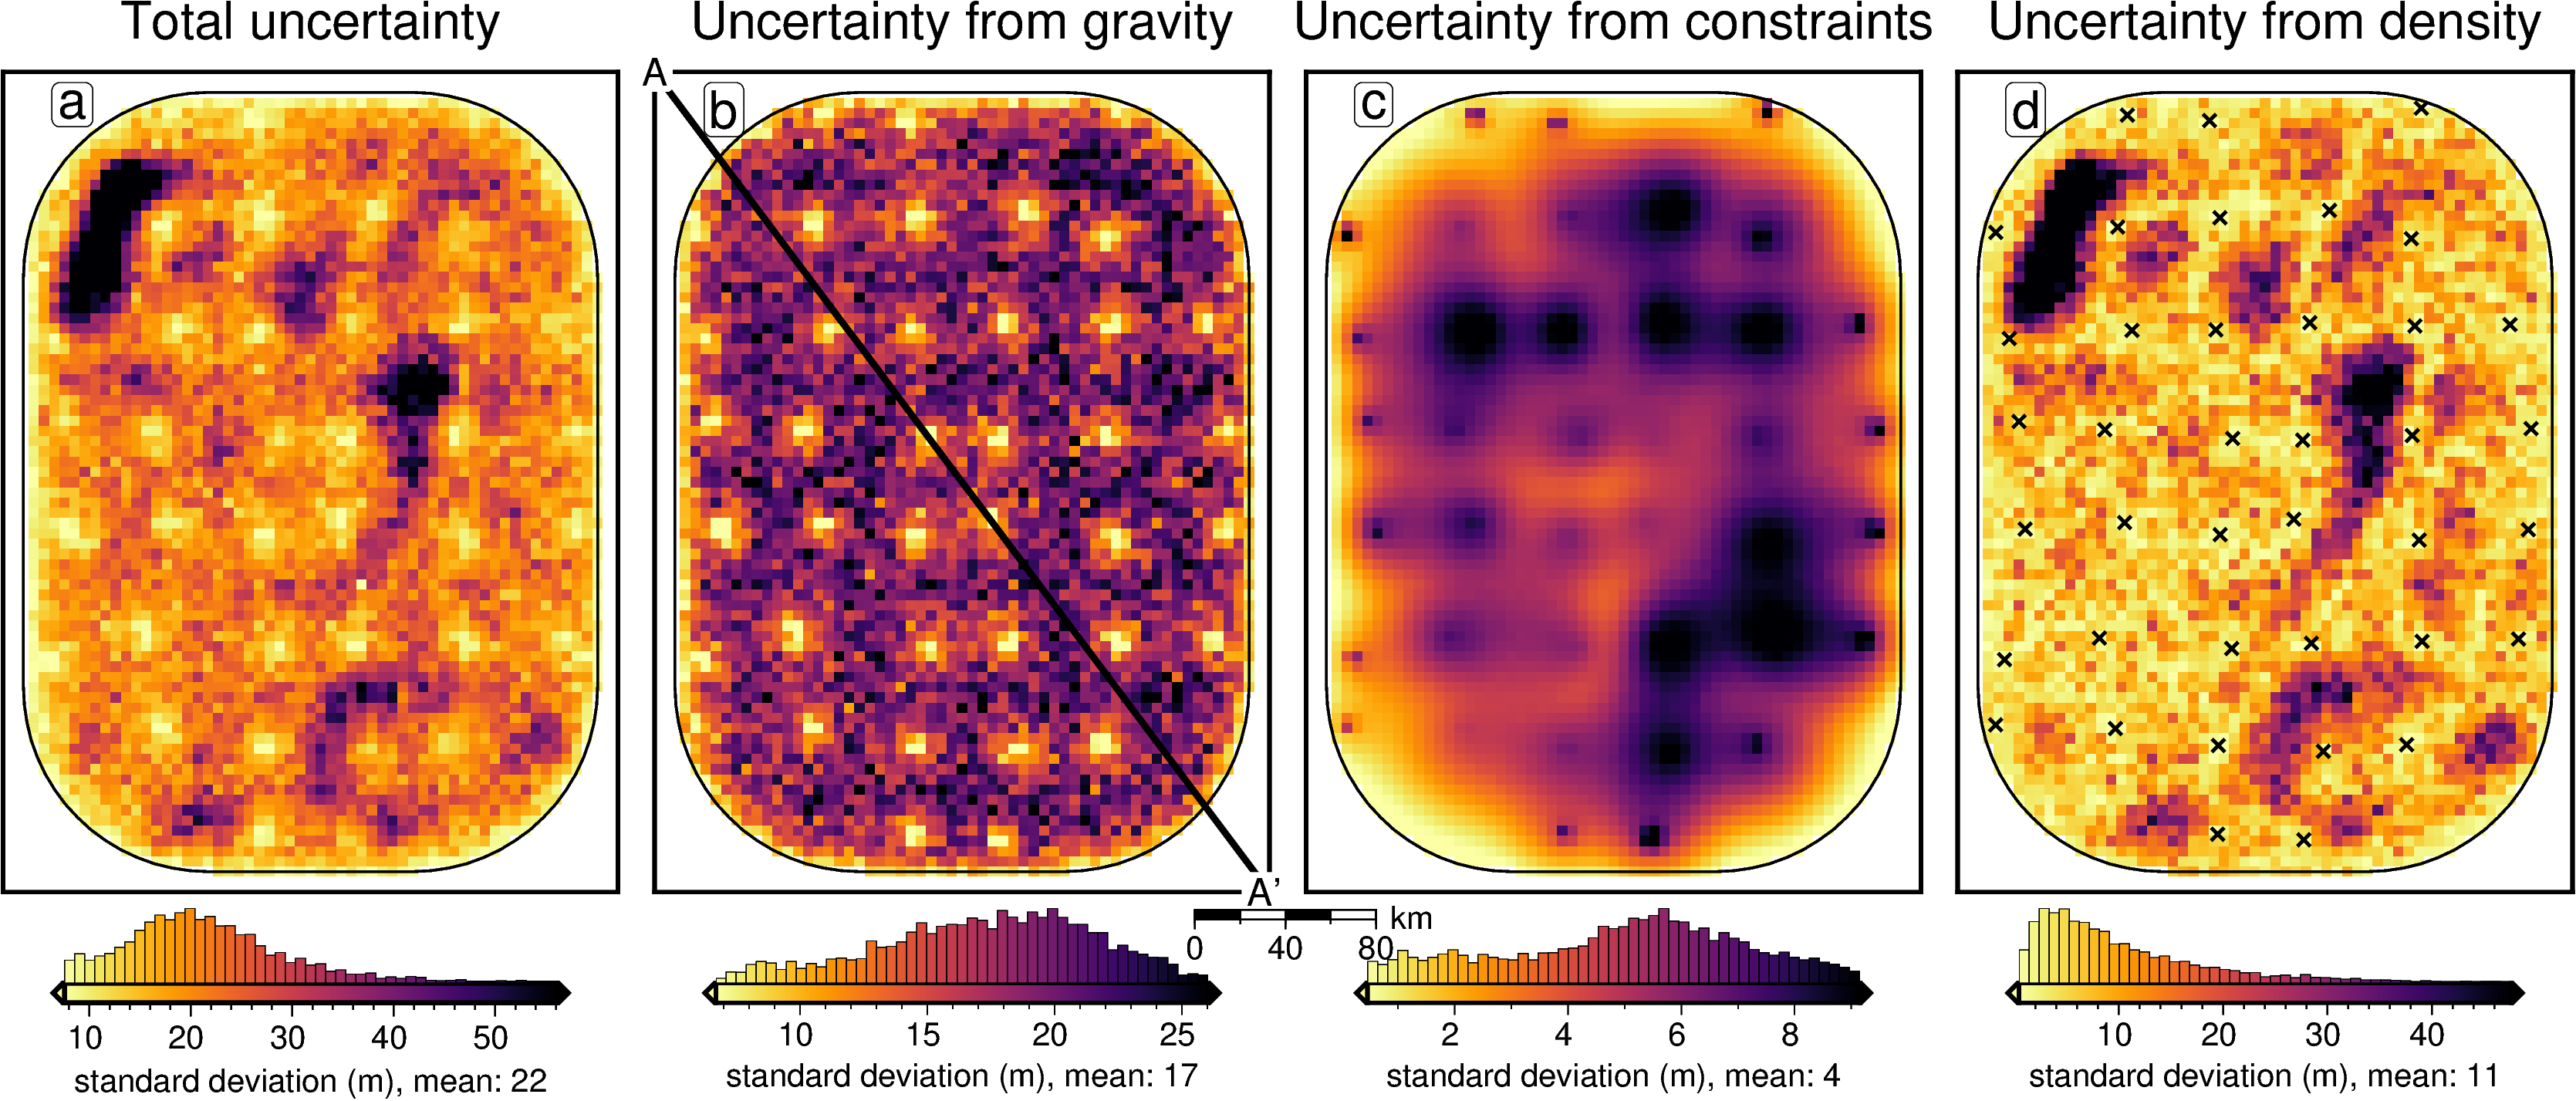
\includegraphics[width=\textwidth]{figures/chp3/chp3_Ross_Sea_monte_carlo.png}
        % \caption{}
    \end{subfigure}
    \begin{subfigure}[t]{.7\textwidth}
        % \addtocounter{subfigure}{3}
        \centering
        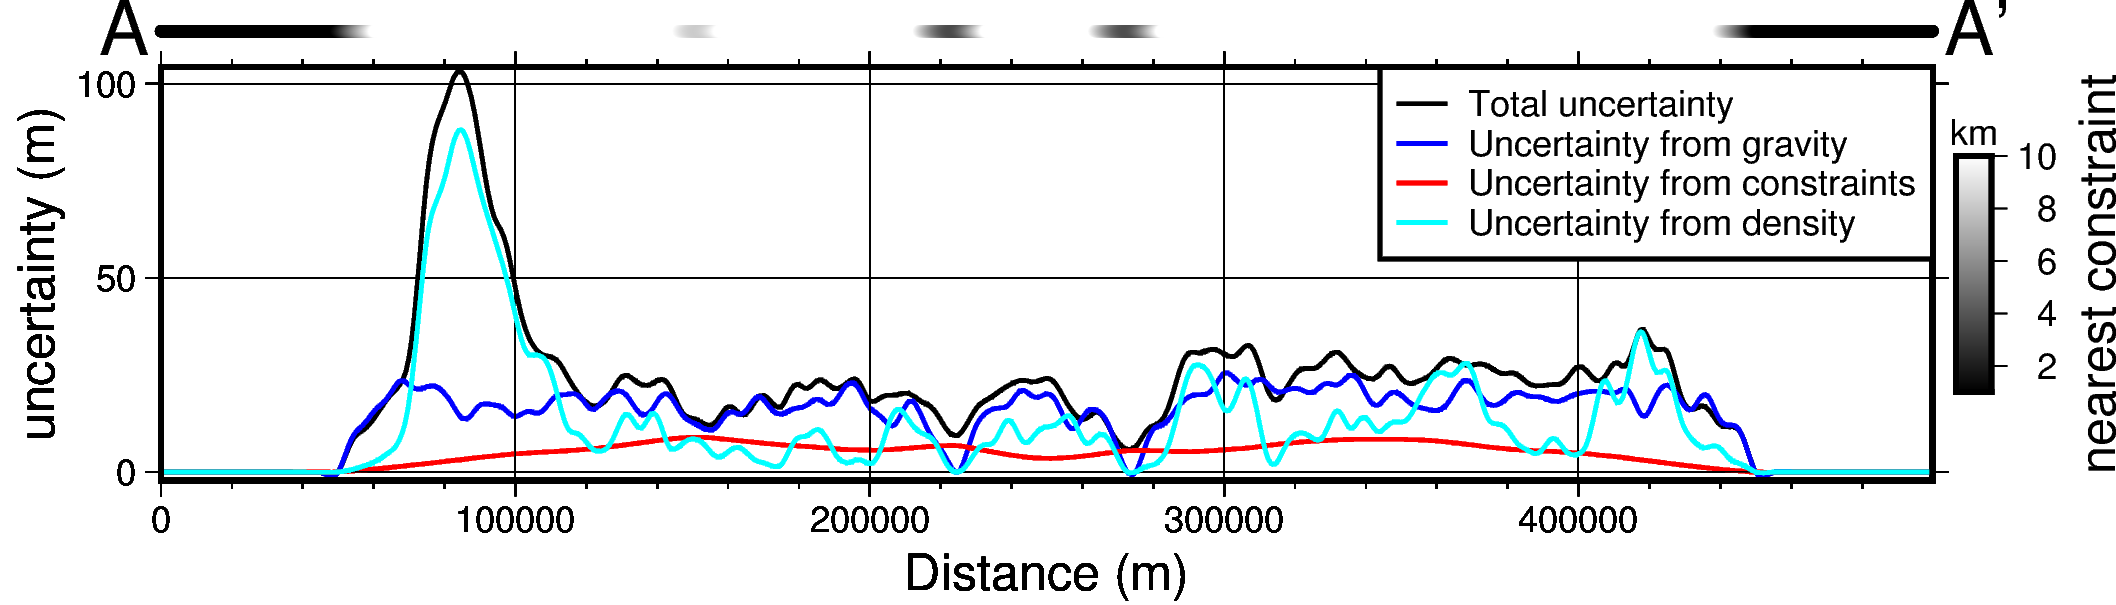
\includegraphics[width=\textwidth]{figures/chp3/chp3_Ross_Sea_monte_carlo_profile.png}
        % \caption{}
    \end{subfigure}
    \caption[Ross Sea Monte Carlo simulation]{Monte Carlo simulation results for the Ross Sea synthetic inversion. Cell-wise weighted standard deviations of all inversions in each simulation. \textbf{a)} Total uncertainty from the sampling of gravity data, constraint depths, and density contrast value. \textbf{b)} Sampling of only the gravity data values. \textbf{c)} Sampling of only the constraint point depths. \textbf{d)} Sampling of only the density contrast. To aid in interpretation, locations outside of the ice shelf have been masked. Constraints within the ice shelf are shown as black crosses in \textbf{d}. \textbf{Lower panel)} Profile from A to A' of the total uncertainty and individual components. Distance to the nearest constraint at each point along the profile shown in black to white colours at top of profile.}
    \label{fig:chp3_Ross_Sea_monte_carlo}
\end{figure}

% \begin{figure}[!ht]
%     \centering
%     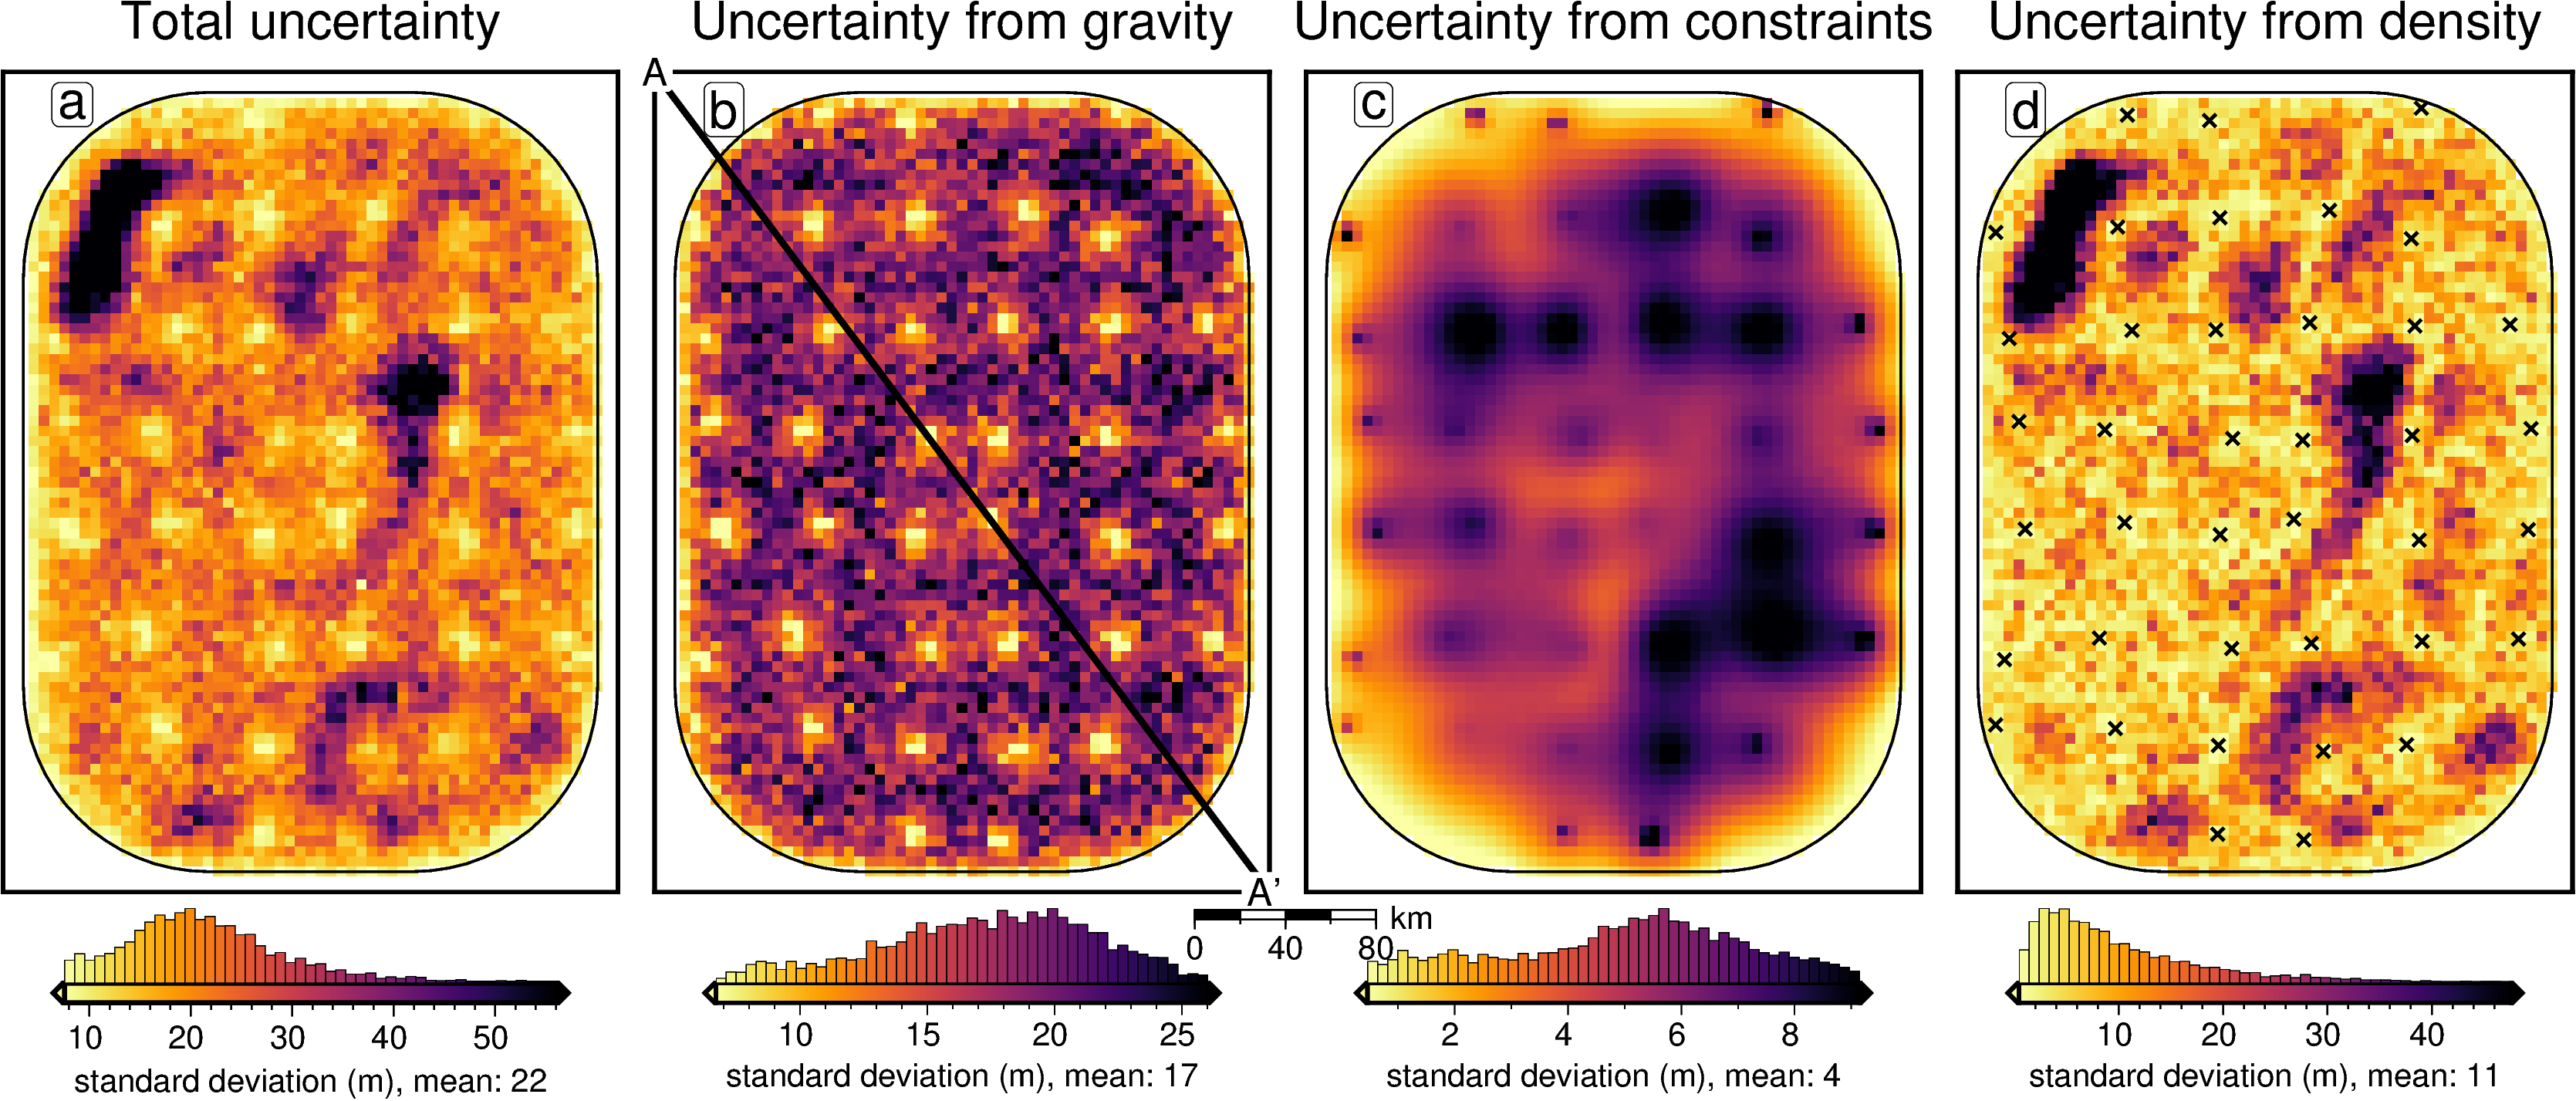
\includegraphics[width=0.95\textwidth]{figures/chp3/chp3_Ross_Sea_monte_carlo.png}
%     \caption{Monte Carlo simulation results for the Ross Sea synthetic inversion. Cell-wise weighted standard deviations of all 100 inversions in each simulation. \textbf{a)} Monte Carlo simulation with a pseudo-random sampling of the gravity data values, the constraint point depths, and the prism density values. \textbf{b)} Sampling of only the gravity data values. \textbf{c)} Sampling of only the constraint point depths. \textbf{d)} Sampling of only the density values. All plots share the same color map. To aid in interpretation, locations outside of the ice shelf have been masked. Constraints outside of the ice shelf are shown as small black crosses and constraints within the ice shelf are shown as large black crosses.}
%     \label{fig:chp3_Ross_Sea_monte_carlo}
% \end{figure}

Four suites of Monte Carlo simulations were run and are shown in \ref{fig:chp3_Ross_Sea_monte_carlo}. Each of the above parameters: gravity, constraints, and densities, were included in their own Monte Carlo simulations, and the fourth simulation included all parameters together. Simulations that included the sampling of the constraint depths required the re-calculation of the starting bathymetry, the starting forward gravity, gravity misfit, regional separation, and finally running the inversion. Simulations that included sampling the density values required recalculating the forward gravity, misfit, regional separation, and running the inversion. Simulations that included the sampling of gravity values only required recalculating the regional field and running the inversion. These values were sampled from their respective distributions using Latin hypercube sampling \citep{jansenmonte1994}. This allows an adequate coverage of the parameter space with only 20 inversions. See Chapter \ref{ch:4} Section \ref{chp4_uncertainty_method} for further details.

\subsection{Effects of constraint spacing} \label{chp3:Ross_Sea_constraints_ensemble}

\begin{figure}[!ht]
\captionsetup[subfigure]{labelformat=empty}
  \centering
    \begin{subfigure}[t]{.6\textwidth}
        \centering
        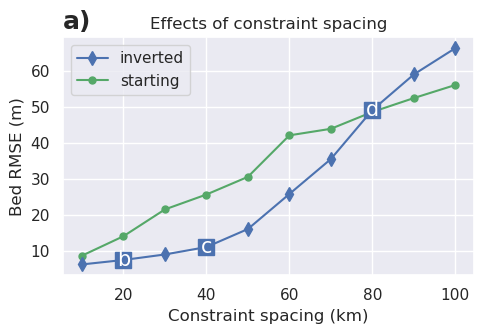
\includegraphics[width=\textwidth]{figures/chp3/chp3_Ross_Sea_constraints_ensemble_graph.png}
        \caption{}
    \end{subfigure}
    \begin{subfigure}[t]{.8\textwidth}
        \centering
        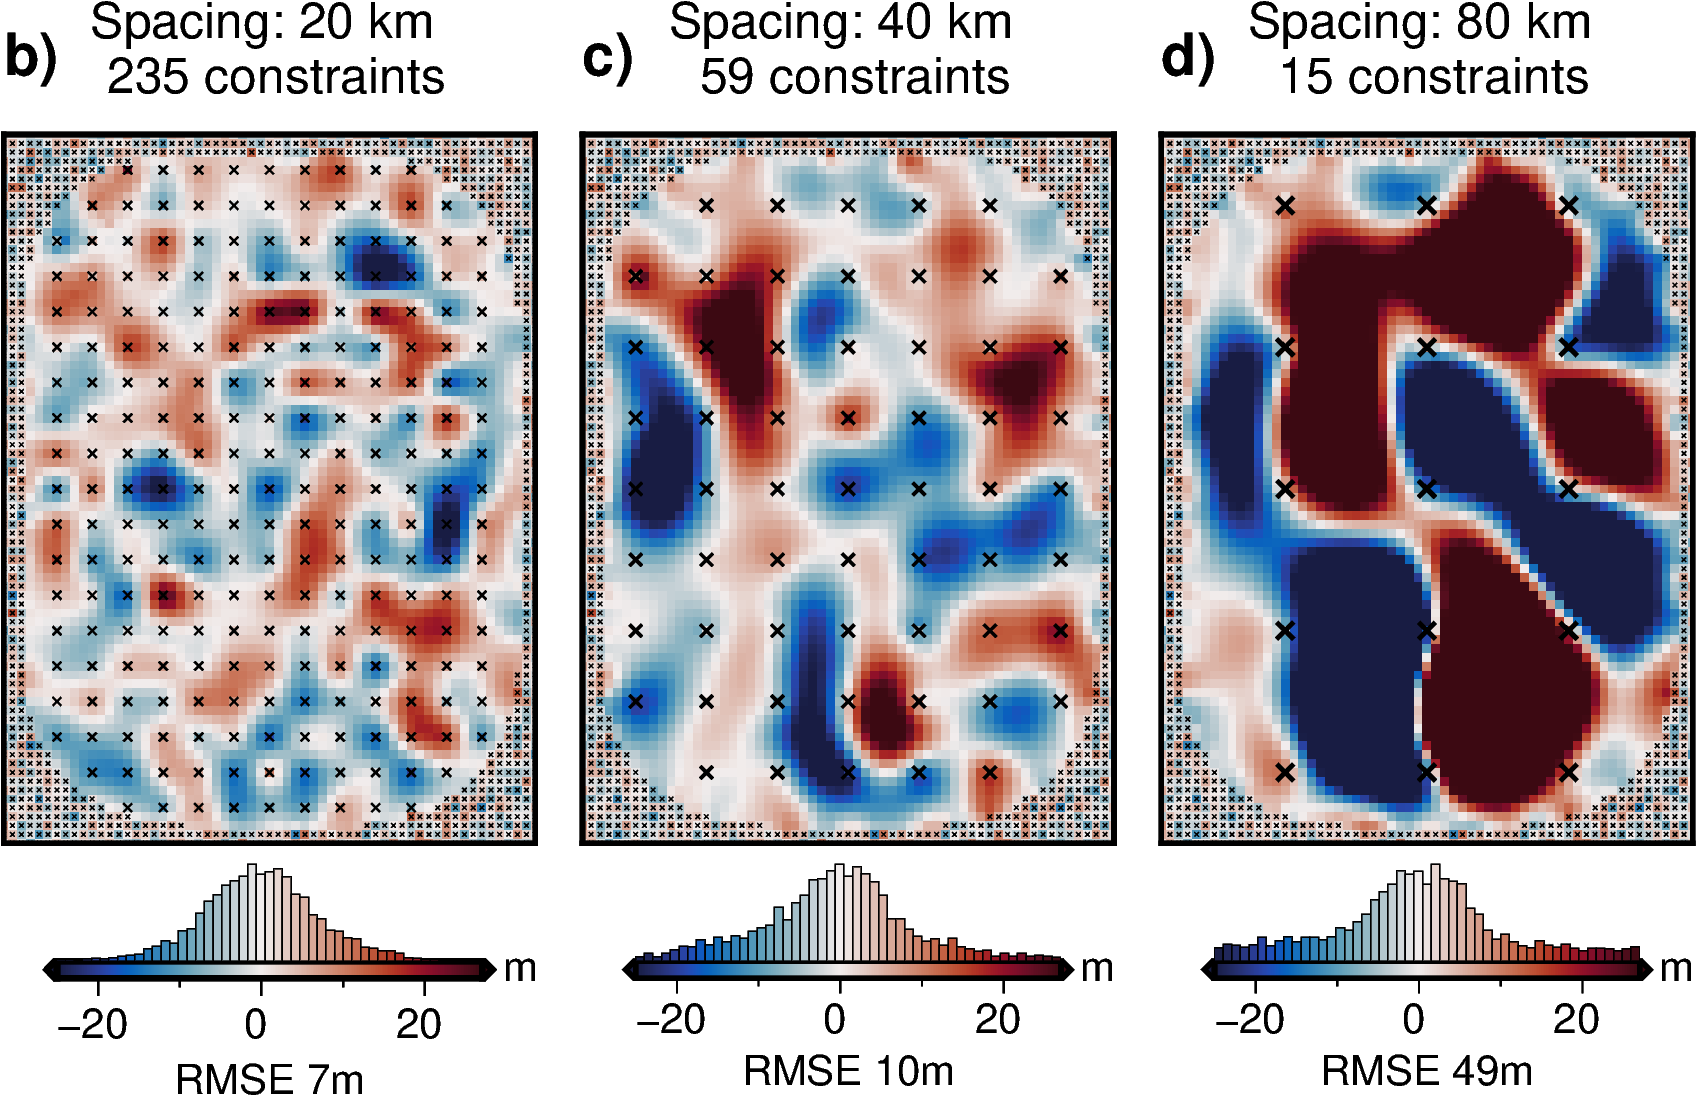
\includegraphics[width=\textwidth]{figures/chp3/chp3_Ross_Sea_constraints_ensemble_errors.png}
        \caption{}
    \end{subfigure}
  \caption[Constraint spacing effects]{Effects of constraint spacing on inversion accuracy. \textbf{a)} Bathymetry error (RMSE) relative to the true bathymetry for 10 different constraint spacing. Green (circles) shows the starting error and blue (diamonds) shows the error after inversion. Labels b, c, and d refer to the three inversion error results shown as subplots. \textbf{b-d)} Inversion error grids for three of the ten configurations of constraints (labelled on a)). Note b-d use the same colour map. Small black crosses show constraints outside the ice shelf, and larger black crosses show inside constraints with the corresponding constraint spacing.}
    \label{fig:chp3_Ross_Sea_constraints_ensemble}
\end{figure}

Here we test the effects of the number and spacing of constraint points on the accuracy of the inversion. The constraints outside the ice shelf are kept as they have been in the previous section, at the same grid spacing as the bathymetry (5~km). Constraints within the ice shelf are re-created on a regular grid, where the spacing of the grid, and thus the number of constraints, is varied from 10~km (959 constraints) to 100~km (9 constraints). The depth of the true bathymetry is sampled at each constraint. As in the previous section, points outside the shelf are contaminated with Gaussian noise with a standard deviation of 5 m. Noise for constraints within the ice shelf is relative to each point's depth (to simulate seismic survey uncertainties). These  noise-contaminated constraint point depths are used in a bi-harmonic spline gridding to create the starting bed for each of the 10 constraint sets. The RMS difference between each of the starting beds and the true bed is shown as green dots in Figure \ref{fig:chp3_Ross_Sea_constraints_ensemble}a. From these starting beds the inversion workflow was conducted, as below:

\begin{enumerate}
    \item The forward gravity of the starting beds were calculated.
    \item The misfits with the observed gravity (Figure \ref{fig:chp3_Ross_Sea_survey}a) were calculated\footnote{To isolate the effects of changing the constraint density, the full resolution observed gravity with no added noise was used here, instead of the synthetic survey gravity.}.
    \item The regional component of the misfit was estimated and removed with the constraint point minimization method.
    \item The residual misfit was inverted with the cross-validation routine.
    \item The difference between each inverted bed and the true bed was found.
\end{enumerate}

Figure \ref{fig:chp3_Ross_Sea_constraints_ensemble} shows the results of this analysis. Subplot a) shows the relationship between constraints spacing and the RMSE with the true bed of the starting bed (green circles) and the final inverted bed (blue diamonds). Three of the inverted bed errors are shown in subplots b-d. See Appendix \ref{appB_Ross_Sea} for plots of the regional separation errors for these three inversions. 


\subsection{Effects of gravity data} \label{chp3:Ross_Sea_gravity_ensemble}

As the above section analyzed the impact of the number of constraint points on the inversion's accuracy, here we investigate the impact of the quality and quantity of input gravity data. Following the methods of the two ensembles presented in the simple synthetic inversion (Figure \ref{chp3:simple_ensemble} \& \ref{fig:chp3_simple_regional_ensemble}), an ensemble of 100 inversions with varying levels of noise and gravity observation spacing's are conducted with this Ross Sea model. The observed gravity data were contaminated with noise as described in the past sections, with 10 levels between 0 and 9\% of the maximum absolute value. To simulate a more spare gravity survey, the previous two ensembles sampled the full-resolution gravity data onto a coarser evenly spaced grid and then re-gridded the sparse data with equivalent sources back to the full resolution of the bathymetry. Here instead of evenly spaced grids, we use airborne flight lines. \\

We use a constant along-line observation spacing of 5~km but vary the spacing between flight lines. The N-S and E-W lines both use the same between-line spacing. The full-resolution gravity is then sampled at these points, and the sparse data is re-gridded to the full resolution (5~km) with equivalent sources. The noise and line spacing changes were applied to the original observed data, and the forward calculation of the starting model, initial misfit calculation, and regional field removal were all repeated. Each model was then inverted with a cross-validation, and the resulting RMS differences with the true bathymetry are shown in Figure \ref{fig:chp3_Ross_Sea_gravity_ensemble}. 

\begin{figure}[!ht]
    \centering
    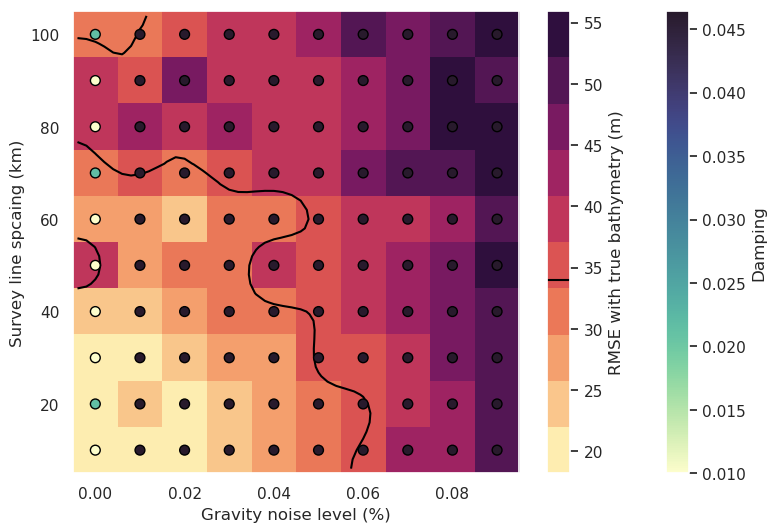
\includegraphics[width=0.9\textwidth]{figures/chp3/chp3_Ross_Sea_gravity_ensemble.png}
    \caption[Ross Sea ensemble of noise levels and gravity spacing]{Ensemble of noise levels and airborne gravity line spacing for the Ross Sea synthetic model. Grid cell colour indicates each inversion's RMSE with the true bathymetry. Circles' colour indicates the optimal damping value found for each inversion's cross-validation. Black line shows the 34~m contour which represents the RMS difference between the true and starting bathymetry (Figure \ref{fig:chp3_Ross_Sea_starting_model}b).}
    \label{fig:chp3_Ross_Sea_gravity_ensemble}
\end{figure}


\section{Discussion}

\subsection{Simple synthetic model}

The simple synthetic model of Section \ref{chp3:simple_model} was introduced to 1) present the basic workflow of the inversion, 2) determine the best options for various components of the inversion and 3) demonstrate the capabilities and limitations of the inversion. The starting bathymetry had an RMS difference with the true bathymetry of 66~m (Figure \ref{fig:chp3_simple_starting_model}). This error demonstrates the limitations of gridding sparse data. Even with a very high spatial constraint density (1 constraint per 160~km\textsuperscript{2}) compared to most ice shelves \citep{fretwellbedmap22013}, simply gridding the constraints greatly misinterpreted the true bathymetry. To reduce this bathymetric error, we presented three inversions, a noise-free full-resolution inversion, a noise-contaminated full-resolution inversion, and a noise-free lower-resolution inversion.

\subsubsection{Inversion results}

All of these inversions (without a regional component) were able to reduce this RMS difference with the true bathymetry to $\sim$~10~m and recover all bathymetric features of interest. We demonstrated that the two methods of calculating the vertical derivative of gravity produced similar results, but the annulus approximation was significantly faster ($\sim$5$\times$). Additionally, for each of these inversions, the weighting grid, based on the distance to the nearest constraints (Figure \ref{fig:chp3_simple_weights}), successfully constrained the resulting inverted bathymetry at the points of prior bathymetry observations. Each inversion's constraint point RMS difference with the true bathymetry was $<\sim$2~m, and the technique avoided any pedestal effect around the constraints in the resulting bathymetries. Interestingly, the inversion with low-resolution (6~km) gravity data yielded a very similar RMSE compared to the inversion with the full-resolution (1~km) data. This demonstrates that for recovering bathymetric features of wavelengths similar to those found in our synthetic model, high-resolution gravity surveys may not be necessary to achieve adequate results from an inversion. 

\subsubsection{Ensemble results}

To test this theory further, we conducted an ensemble of 100 inversions with 10 levels of noise contamination and 10 gravity survey resolutions. The resulting RMS difference of each inversion with the true bathymetry is shown in Figure \ref{fig:chp3_simple_ensemble}. All inversions in this ensemble, including the worst-case scenario of 9\% noise and a gravity observation grid of 10$\times$ the bathymetry spacing, still resulted in an RMS difference lower than that of the starting bathymetry (66~m). It is worth noting that this metric for the accuracy of the inversion, the root mean squared (RMS) difference with the true bathymetry, is used to give extra weighting to the outlier errors, as opposed to using a mean average error (MAE). These outliers typically include the features of interest in a bathymetry inversion. Figure \ref{fig:chp3_simple_ensemble_lines}a shows these ensemble results grouped by cell size. For each cell size value (colour of lines), the inverted bed RMSE for the range of noise levels is shown. This shows a roughly linear relationship between noise and RMSE, regardless of cell size. This means there is a continuous improvement in the inversion's accuracy with lower levels of noise. Conversely, figure \ref{fig:chp3_simple_ensemble_lines}b shows these ensemble results grouped by the noise level. For each noise level (colour of lines), the inverted bed RMSE for the range of cell sizes is shown. This shows an exponential relationship between gravity survey resolution and RMSE. This exponential relationship is strongest for low noise levels. This means inversion accuracy greatly benefits from increasing the survey resolution (decreasing the cell size), but this benefit diminishes once the survey resolution is at a certain point. Here, surveys at or below $\sim$6~km resolutions result in a diminishing improvement in RMSE. The linear relationship between noise and RMSE, and the exponential relationship between resolution and RMSE can also be seen by the spacing of lines in either figure. The close spacing of the low-cell-size lines (purples) in Figure \ref{fig:chp3_simple_ensemble_lines}a show the diminishing improvements at small cell size surveys, while the continuous spacing of lines in Figure \ref{fig:chp3_simple_ensemble_lines}b shows the linear relationship. \\

\begin{figure}[!ht]
  \centering
    \begin{subfigure}[t]{.48\textwidth}
        \centering
        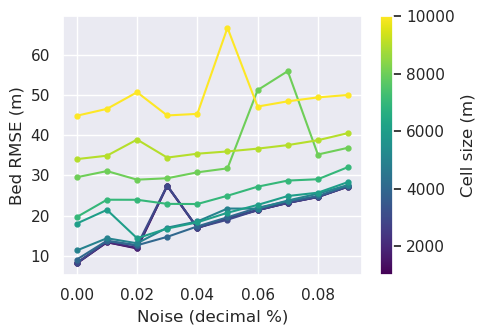
\includegraphics[width=\textwidth]{figures/chp3/chp3_simple_ensemble_noise_lines.png}
        \caption{}
    \end{subfigure}
    \begin{subfigure}[t]{.48\textwidth}
        \centering
        \includegraphics[width=\textwidth]{figures/chp3/chp3_simple_ensemble_cellsize_lines.png}
        \caption{}
    \end{subfigure}
  \caption[Grouped synthetic inversion ensemble]{Ensemble results for the simple synthetic inversion, grouped by \textbf{a)} gravity survey cell size, and by \textbf{b)} noise level. Each line in a) corresponds to a row of Figure \ref{fig:chp3_simple_ensemble} and each line in b) corresponds to a column.}
    \label{fig:chp3_simple_ensemble_lines}
\end{figure}

In a typical gravity survey, there is often a trade-off between the number of observations made and the quality (noise) of the data. This is due to the time restrictions of both the total data collection period (i.e. the length of a field season in Antarctica), and the necessity to repeat base-station measurements to account for instrument drift. Collecting more data in the same time period inevitably results in increased noise. At a certain point, this increased noise will have a greater negative effect on the inversion results, than will be counteracted by the increased amount of data. These are important considerations for survey design. Figure \ref{fig:chp3_simple_ensemble_lines}b shows that for a given noise level, there is little benefit in increasing the gravity survey resolution from $\sim$6~km to 1~km. For this survey domain (60~$\times$~80~km), a 6~km resolution results in $\sim$130 gravity station, while with a 1~km resolution, this increases to 4800 observation points. Simplistically speaking, if keeping total survey time constant, this means at 6~km spacing as opposed to 1~km spacing, either $\sim$36$\times$ more area could be surveyed, or higher quality data could be collected, with shorter base station loops, more repeated ties, and more careful measurements. \\

The results from the noise-contaminated inversion (Figure \ref{fig:chp3_simple_noise_results} \& \ref{fig:chp3_simple_CV_and_profile}b) show that this gravity noise is directly reflected in the inversion results. For this reason, data, either the observed data or the residual misfit, is typically low-pass filtered prior to inversion \citep[i.e.][]{boghosianresolving2015, yangocean2020}. This is typically done with either a time-based filter for airborne surveys, or a spatial filter \citep{jordanaerogravity2010}. With this filtering, there is a trade-off between removing the noise and removing the true signal. Due to this, we have chosen to omit the filtering in these synthetic examples.

\subsection[Regional component]{Simple model with a regional component\sectionmark{Regional component}}

\subsubsection{Regional separation methods}

The addition of a regional component to the observed gravity data adds a major complexity to the inversion workflow. The actual inversion remains the same, but this regional component must be estimated and removed beforehand. We tested four methods of regional estimation; 1) a low-pass filter, 2) fitting a polynomial trend to the data, 3) predicting the data with a set of deep point sources, and 4) attributing the entire misfit value to the regional field at constraint points and interpolating between these values. Figure \ref{fig:chp3_simple_regional_comparison} compares the inversion results of each of these methods. While each method recovered the short wavelengths bathymetry features, the misestimation of the true regional field for each method introduced long-wavelength errors in the inversion results. We show that the constrain point minimization method most accurately estimated the region, and thus produced the best inversion results. For the simple regional field used here, the filter and trend methods achieved reasonable results, but the effectiveness of these methods is expected to be reduced with more complex regional fields associated with real data. \\

While the constraint point minimization worked best for this model, each of these methods may work better in specific scenarios. All the methods except the equivalent source method require the gravity data to be gridded over the entire region of interest. For sparse gravity surveys the interpolation required may introduce large errors. For this scenario, the equivalent source technique is likely the most appropriate. In scenarios with few bathymetry constraints and where the regional field is expected to be simple, the trend and low-pass filter methods are efficient and can be effective. However, if there are distributed bathymetry constraints, such as in this synthetic scenario, constraint point minimization is likely the best choice. This technique will only effectively remove regional anomalies with a wavelength equal to or greater than the average constraint spacing. If the constraints are sparse relative to the expected regional anomaly wavelengths, this method will underestimate the regional component. Lastly, if the bathymetry contains long-wavelength features which would result in long-wavelength anomalies, the trend, filter, and equivalent source techniques may include these in the regional removal. Therefore, the inverted bathymetry, while recovering the super-imposed short-wavelength bathymetry features, will underestimate the long-wavelength features. It is for these reasons that regional separation is perhaps the most important aspect of a bathymetry inversion. 

\subsubsection{Constraint point minimization}

This constraint point minimization technique requires the gridding of sparse measurements of the regional field. We explored the impact of this gridding process on the resulting inversion. Figure \ref{fig:chp3_simple_regional_gridding_comparison} shows the results of four different gridding processes. Minimum curvature gridding without tension (tension of 0, Figure \ref{fig:chp3_simple_regional_gridding_comparison}a) produces a smoothly varying surface at the constraints but introduces artificial minima and maximum at points far from any constraints. This erroneous effect is minimized with a higher tension factor. Using a tension factor of 1, figure \ref{fig:chp3_simple_regional_gridding_comparison}c shows the limited erroneous minima and maxima, but this added tension results in high gradients in the surface immediately near the constraint points (Figure \ref{fig:chp3_simple_regional_gridding_comparison}g). These high gradients in the resulting residual anomalies create a \textit{ringing} effect in the inverted bathymetry (Figure \ref{fig:chp3_simple_regional_gridding_comparison}k). For these reasons, an intermediate tension factor of 0.25 is suggested for potential field data. While this limits the negative effects of both low and high tension, there are still false minima and maxima (Figure \ref{fig:chp3_simple_regional_gridding_comparison}b), and high gradients at the constraints (Figure \ref{fig:chp3_simple_regional_gridding_comparison}f). The last gridding technique uses bi-harmonic splines. The optimal damping parameter associated with this technique is chosen from a cross-validation of the constraint points. This technique, while being more computationally expensive, solves both issues of tensioned minimum curvature. 

\subsubsection{Inversion results}

\begin{figure}[!ht]
    \centering
    \includegraphics[width=.7\textwidth]{figures/chp3/chp3_simple_regional_bed_error.png}
    \caption[Synthetic inversion error and regional error]{Source of inverted bathymetry error for the simple synthetic model with a regional field. \textbf{a)} Inverted bathymetry error from Figure \ref{fig:chp3_simple_regional_results}b. \textbf{b)} Error in the estimation of the regional component of gravity from comparison with the true regional component (Figure \ref{fig:chp3_simple_regional_gravity}b). Black crosses show constraint points. Colourmaps are inverted to highlight the similarities and the median has been removed from the regional error.}
    \label{fig:chp3_simple_regional_bed_error}
\end{figure}

With both the optimal regional separation method and the optimal gridding method determined, we performed a cross-validated inversion with the remaining residual misfit. This inversion was able to recover all the short-wavelength bathymetry features but introduced some long-wavelength errors. Figure \ref{fig:chp3_simple_regional_bed_error} shows the inverted bathymetry error alongside the error in estimating the regional component of gravity. Comparing these shows that almost all of the inverted bathymetry error is tied to the inaccuracies of determining the regional component. the remaining error is all minor short-wavelength features, mostly around constraint points. They appear to result from the weighting grid implementation of regularization. Since the errors in the regional estimation are the dominant source of error in most inversions, as shown above, and by other Antarctic bathymetry inversions \citep{brisbourneseabed2014}, we have shown these details of the gridding process are a vital and often overlooked step in many studies. 

\subsubsection{Ensemble results}

As with the simple model, an ensemble of noise and gravity survey spacing experiments were performed with this model containing a regional component. The lowest resulting RMS difference with the true bathymetry was raised from values of $\sim$10~m for the inversion without the regional component, to the lowest value of $\sim$~40 m with the additional regional component. The black line in Figure \ref{fig:chp3_simple_regional_ensemble} shows the 66~m contour, which represents the RMS difference between the true and starting bathymetries. Inversions that fall outside (above) this line resulted in a worse bathymetry than the starting model. This shows that for this model, inversion is only worth conducting if the gravity survey has a spacing less than $\sim$9~km ($\sim$9$\times$ the spacing of the desired bathymetry resolution). Figure \ref{fig:chp3_simple_regional_ensemble_lines} show these ensemble results grouped by cell size and noise level. There is a linear relationship between gravity noise and the resulting bathymetry RMSE, for all gravity survey spacings. There is an approximately exponential relationship between gravity survey resolution (cell size) and resulting bathymetry RMSE. The degree of this exponential relation decreases with increased noise. \\

For this model, the \textit{elbow} of the exponential curves in Figure \ref{fig:chp3_simple_regional_ensemble_lines}b is at $\sim$ 6~-~8~km survey resolutions (6-8$\times$ bathymetry resolution). This suggests that for a survey resolution finer than $\sim$8~km, there is little benefit in collecting more data. This is supported by the close spacing of low-cell-size lines (purples) in Figure \ref{fig:chp3_simple_regional_ensemble_lines}a. The effort would be better spent collecting data over a wider region, reducing noise in the data, or if possible collecting more bathymetric constraints.

\begin{figure}[!ht]
  \centering
    \begin{subfigure}[t]{.48\textwidth}
        \centering
        \includegraphics[width=\textwidth]{figures/chp3/chp3_simple_regional_ensemble_noise_lines.png}
        \caption{}
    \end{subfigure}
    \begin{subfigure}[t]{.48\textwidth}
        \centering
        \includegraphics[width=\textwidth]{figures/chp3/chp3_simple_regional_ensemble_cellsize_lines.png}
        \caption{}
    \end{subfigure}
  \caption[Grouped synthetic inversion with regional ensemble]{Ensemble results for the synthetic inversion with a regional component, grouped by \textbf{a)} gravity survey cell size, and by \textbf{b)} noise level. Each line in a) corresponds to a row of Figure \ref{fig:chp3_simple_regional_ensemble} and each line in b) corresponds to a column.}
    \label{fig:chp3_simple_regional_ensemble_lines}
\end{figure}

\subsection{Ross Sea model}

The Ross Sea semi-realistic model was created to better emulate the gravity and bathymetries expected for ice shelves. A few extra complexities were added to this model compared to the purely synthetic models. An ice shelf border was included, with a high density of constraints outside of the border, and sparse constraints within. All the constraints had an associated uncertainty, instead of directly sampling the true bathymetry depths. The observed gravity was calculated along the flight paths of a typical airborne survey, instead of along a uniform grid. The main inversion in this section had 2\% noise added and had flight lines with 50~km N-S spacing and 15~km E-W spacing. The inversion successfully reduced the starting bathymetry error from an RMSE of 34~m to 23~m. The resulting bathymetry shows a recovery of most of the lost bathymetry features, but some noise from the gravity data has been introduced into the bathymetry. Sharp bathymetry features (upper left corner) and smooth features were both recovered. The constraint points were relatively evenly distributed (Figure \ref{fig:chp3_Ross_Sea_starting_model}d), resulting in a relatively even distribution of bathymetry misfits. \\

Of these errors, the largest were located at the gaps in the synthetic survey where there were missing flight lines (Figure \ref{fig:chp3_Ross_Sea_survey}b). To understand the cause of the remaining errors, we compare the inverted bathymetry error with the regional separation error (Figure \ref{fig:chp3_Ross_Sea_regional_bed_error}). The strong correlation between these two grids shows that the majority of errors in the inversion are tied to the miscalculation of the regional field, as was seen in the simple synthetic inversion with a regional field. The remaining errors appear to be from the flight line gaps and noise in the gravity data. 

\begin{figure}[!ht]
    \centering
    \includegraphics[width=.7\textwidth]{figures/chp3/chp3_Ross_Sea_regional_bed_error.png}
    \caption[Ross Sea inversion error and regional error]{Comparison of the inverted bathymetry error and the error in the regional field estimation. \textbf{a)} Inverted bathymetry error from Figure \ref{fig:chp3_Ross_Sea_results}b. \textbf{b)} Error in the estimation of the regional component of gravity from comparison with the true regional component (Figure \ref{fig:chp3_Ross_Sea_layers_and_forwards}d). Black crosses show constraint points. Colourmaps are opposed to highlight the similarities and the median has been removed from the regional error.}
    \label{fig:chp3_Ross_Sea_regional_bed_error}
\end{figure}

\subsubsection{Effects of the gravity data} \label{chp3_effect_of_gravity_noise}

The ensemble of gravity data noise levels and flight line spacings from Section \ref{chp3:Ross_Sea_gravity_ensemble} shows the relative importance of these two aspects of a gravity survey. As for the previous ensembles, Figure \ref{fig:chp3_Ross_Sea_gravity_ensemble_lines} shows these results grouped by line spacing and by the noise level. For the Ross Sea model, both factors have a roughly linear relationship with inverted bathymetry error. The slopes for the lines of best fit for Figure \ref{fig:chp3_Ross_Sea_gravity_ensemble_lines}a and b means the inversion RMSE increases by $\sim$10~m for either a 4\% increase in the noise level or a 60~km increase in the average flight line spacing. The inversions with a small line-spacing (purple lines) of Figure \ref{chp3:Ross_Sea_gravity_ensemble}a are closely grouped, relative to the higher line spacings. This shows that at already low line spacings (40~km) there may be little benefit to reducing the line spacing further. Conversely, there is a larger spread for the low noise inversions (purple lines) in Figure \ref{chp3:Ross_Sea_gravity_ensemble}b. This shows that even at low noise levels, further decreases may still provide important improvements to the inversion outcome. As in the previous ensemble results, for a field application, this demonstrates the important tradeoff between quantity and quality of gravity data. \\

\begin{figure}[!ht]
  \centering
    \begin{subfigure}[t]{.48\textwidth}
        \centering
        \includegraphics[width=\textwidth]{figures/chp3/chp3_Ross_Sea_gravity_ensemble_noise_lines.png}
        \caption{}
    \end{subfigure}
    \begin{subfigure}[t]{.48\textwidth}
        \centering
        \includegraphics[width=\textwidth]{figures/chp3/chp3_Ross_Sea_gravity_ensemble_spacing_lines.png}
        \caption{}
    \end{subfigure}
  \caption[Grouped Ross Sea inversion with regional ensemble]{Ensemble results for the Ross Sea inversion, grouped by \textbf{a)} gravity survey line spacing, and by \textbf{b)} noise level. Each line in a corresponds to a row of Figure \ref{fig:chp3_Ross_Sea_gravity_ensemble} and each line in b corresponds to a column. Red lines show the line of best fit, with their slopes shown in the upper left corners.}
    \label{fig:chp3_Ross_Sea_gravity_ensemble_lines}
\end{figure}

These specific relationships between noise, line spacing, and inversion error, while not applicable to all survey configurations, show the importance of choosing an appropriate survey design. This analysis with synthetic data could be included in a pre-survey plan, to explore the effects of differing survey configurations. 

\subsubsection{Effects of the constraints} \label{chp3_effect_of_constraints}

These synthetic inversions have shown that the removal of the regional field presents the biggest challenge for gravity inversions for bathymetry. The most robust technique for removing the regional field requires a distribution of points of known bathymetry across the inversion region. Since the largest errors in the inverted bathymetries occur at the largest distance to constraints, an even distribution of constraints will best be able to estimate the regional field. Section \ref{chp3:Ross_Sea_constraints_ensemble} explored the effects of varying the numbers of constraints, while keeping the remaining components of the inversion constant. Figure \ref{fig:chp3_Ross_Sea_constraints_ensemble}a shows the bathymetry RMSE with the true bathymetry both before (green) and after (blue) the inversion is conducted. \\

Figure \ref{fig:chp3_Ross_Sea_constraints_ensemble}a shows for this synthetic model that for average constraint spacing's less than $\sim$20~km there is little improvement made by running an inversion. This is due to the starting bathymetry model already being relatively accurate, with the inversion only producing minor adjustments between constraint points. At the other end of the spectrum, with constraint densities greater than $\sim$70~km, the inverted bathymetry has an error similar to or higher to the un-inverted bathymetry. This is due to the inaccuracies in calculating the regional field with only very sparse constraints. For these scenarios, the errors introduced by the inversion are greater than the errors of simply interpolating the constraint points. The inverted bathymetry error curve (Figure \ref{fig:chp3_Ross_Sea_constraints_ensemble}a) shows that for this survey, once below a certain constraint spacing ($\sim$30~km) there is little benefit to having additional constraints. 

\subsubsection{Uncertainties}
We have demonstrated that the majority of the inverted bathymetry error is related to the estimation of the regional component of gravity. Without knowing the true regional component, as we do in these synthetic examples, estimating the uncertainty in the interpolation between constraint points of the regional field is difficult. The uncertainty of each grid cell is likely strongly dependant on the distance to the nearest constraint, as well as the depth uncertainties of these nearby constraints. While we show this to be true with our synthetic models, a quantitative method of predicting this uncertainty has yet to be implemented here. The field of conventional bathymetry surveying has developed uncertainty analysis tools that may be applicable to this \citep{bourgeoisachieving2016}. \\

These tools are able to account for both the depth uncertainty of each measurement, and the distance of each grid cell to the nearest measurement. Future work will benefit from a quantitative assessment of the uncertainty of gridding the regional field from the constraint point values. While the uncertainty of the regional removal accounts for the majority of the uncertainty of the inverted bathymetry, it is technically completed before the inversion and is thus not a component of the inversion uncertainty. To address the uncertainty resulting from the inversion process, we introduced a suite of Monte-Carlo simulations in Section \ref{chp3:monte_carlo}. The results in figure \ref{fig:chp3_Ross_Sea_monte_carlo} show a mean uncertainty for the entire region of 22 m. The majority of this uncertainty is attributed to the uncertainty in the gravity data, as shown by histograms of Figure\ref{fig:chp3_Ross_Sea_monte_carlo}. Here we discuss the significance of each component of the uncertainty analysis:

\begin{enumerate}
    \item \textbf{Gravity uncertainty:} The uncertainties in the gravity data result in a relatively uniform bathymetry uncertainty across the region of 17~m. A simple calculation with the Bouguer slab formula with a density contrast of 1276~kg~m\textsuperscript{-3} and our assumed gravity uncertainty of 0.612~mGal (\%2 max absolute value) gives a value of 11.5~m ($\Delta g_{boug}= 4.18\text{e-}5 \rho h$). This may show the conventionally used Bouguer slab approximation is underestimating the true uncertainty in inversions resulting from gravity data uncertainty. This uncertainty is lowest at the constraints, due to the use of the weighting grid in the inversion. 

    \item \textbf{Constraint depth uncertainty:} The contribution to the bathymetry uncertainty from the depth uncertainty of the constraint points is small, with a mean of $\sim$4~m. This uncertainty resulting from the constraints is also concentrated around the constraint points. This shows improving the constraint point uncertainties will not greatly improve the inversion, and will only improve it in the immediate vicinity of constraints. 

    \item \textbf{Density uncertainty:} The bathymetry uncertainty component resulting from the prism densities is heterogeneous, with some spatially limited, but large values. The mean value is $\sim$11~m, but some areas are up to 50~m. These high uncertainties are strongly correlated with the error in the starting bathymetry (Figure \ref{fig:chp3_Ross_Sea_starting_model}b). This is due to the change in density contrast resulting in a change in the total bathymetry correction calculated in the inversion. In other words, the residual misfit can be minimized by a large surface correction with a low-density contrast or a small surface correction with a large-density contrast. 
\end{enumerate}

The combined Monte-Carlo simulation (Figure \ref{fig:chp3_Ross_Sea_monte_carlo}a) shows the expected features of an uncertainty map. It has a base level uncertainty similar to the Bouguer slab thickness from the assumed gravity uncertainty, it is generally lowest at the constraints and highest in the large constraint gaps, and it is high where the inversion has produced a large change from the starting model.

\section{Future work}

Running this inversion with the various synthetic models gave us the ability to assess the inversion performance. From this assessment, we have determined several components which would benefit from additional investigation. 

\begin{enumerate}
    % \item Test the effects of the relative strengths of the regional and residual components.
    \item Implement an additional cross-validation routine to estimate the optimal density contrast, as in \citet{uiedafast2017}. Here, we have used the same density contrasts for the creation of the observed gravity data and for the inversion itself. In a non-synthetic scenario, this contrast would need to be estimated.
    \item Test the effects of flight line orientation relative to the dominant trend of geologic structures.
    \item Implement a more robust method of enforcing the constraint points. This may likely be in the form of a bounded least squares solver or some form of manipulation of the Jacobian matrix. 
    \item Quantify the uncertainty of the regional separation process. This will likely include techniques used in conventional bathymetry surveying \citep{calderdevelopment2017, bourgeoisachieving2016}, or a sequential Gaussian simulation \citep{perozziquantitative2021}.
    % \item Include the equivalent source gridding of the observed gravity data in the Monte Carlo analysis to see the effects of the entire workflow, not just the inversion.
    % \item Perform a three-way comparison of the effects of constraint spatial density, gravity survey spacing, and gravity noise.
    \item Testing the effects of pre-filtering the gravity data, either spatially or temporally, to remove the effects of noise \citep{jordanaerogravity2010}.
\end{enumerate}

\section{Conclusion}

With the goal of modelling the bathymetry beneath a floating ice shelf, we present a geometric gravity inversion method that 1) adheres to prior bathymetry point measurements, within their uncertainties, 2) produces a smooth and realistic bathymetry, 3) accounts for the regional gravity field and 4) is computationally efficient and fully-open source. To demonstrate the effectiveness, as well as the limitations, we conducted a series of inversions using synthetic and semi-realistic data. These inversions showed the importance of accurately estimating and removing the regional component of gravity prior to the inversion. We showed that for the constraint arrangement for many Antarctic ice shelves, the optimal method for estimating this regional field is with a constraint-point minimization. In addition, we further explored this method by testing various gridding (interpolation) techniques and found a clear increase in performance when using a cross-validated bi-harmonic spline instead of the typically used tensioned minimum curvature. \\

Here we reiterate a few of the key findings from this chapter:
\begin{enumerate}
    \item 
    Estimating and removing the regional component of gravity for typical inversion scenarios is the most important aspect of the inversion procedure. For typical bathymetry inversions, the optimal method for estimating the regional field is constraint point minimization.
    \item 
    When collecting data for an inversion, it is best to aim for quality over quantities for the gravity data, and conversely, quantity over quality for bathymetry constraint measurements.
    \item 
    We provide general guidelines on the optimal ranges of constraint density, gravity survey line spacing, and gravity noise, for which conducting an inversion is suitable. 
\end{enumerate}

Testing the various models with differing levels of gravity noise and numbers of gravity observation points highlights an important factor in planning a gravity survey. We show for the Ross Sea synthetic model, which likely emulates the scenario expected from many Antarctic ice shelves, \textbf{there are diminishing returns for average flight line spacings smaller than $\sim$40~km} if the goal is to recover bathymetry features typical of the Ross Sea. \textbf{However, the inverted bathymetry's accuracy is strongly affected by noise in the gravity data.} With this, the typically airborne survey focus on quantity over quality may need to be reassessed. If 40~km spaced flight lines produce similar results to 20~km lines, flying half the number of lines will save a significant amount of time. This time could be used to either expand the area of the survey or reduce the noise in the data. Reducing the data noise for an airborne survey may not always be feasible, but a few measures may be taken to attempt this, all of which are aided by the increased survey time allowed by reducing the number of flight lines. These include repeating lines or sections which are noisy, limiting flights to good weather windows, increasing the number of tie-lines, making shorter loops for base-station ties, or flying at lower altitudes and or ground speeds.  \\

\textbf{The previous measurements of bathymetry, referred to as the constraints, are a vital part of an inversion for bathymetry.} Due to the non-uniqueness of an inversion, there are an infinite number of inverted bathymetry models which will equally match the observed data. These constraints provide the ground truth necessary to confidently chose a model out of these infinite choices. Additionally, if not more importantly, they provide the primary method of accounting for the regional component of gravity. Since this is shown to be the largest source of uncertainty, the constraints are the most important aspect of the inversion. We tested the effects of varying the spatial density of the constraint points. The results (Figure \ref{fig:chp3_Ross_Sea_constraints_ensemble}) show the range of constraint point spacings for the Ross Sea synthetic model which justifies conducting a gravity inversion if the goal is to recover bathymetry with a 5~km resolution. \\

\textbf{The optimal constraint spacing is $\sim$20-70~km.} Smaller spacing values already have an adequate amount of information and little is gained over a simple interpolation of the data. At spacings larger than $\sim$70~km, the errors in estimating the regional field are larger than the improvements made by the inversion. These values, while specific to the Ross Sea scenario, provide an important context for the feasibility of conducting bathymetry inversions. Taken together with the above assessment of the relative importance of gravity data noise and density, some general guidelines are provided. \\

As long as the gravity data is on the order of magnitude of 2-4$\times$ the spacing of the desired bathymetry resolution, and the noise levels are low, \textbf{efforts should be focused on collecting more bathymetry measurements.} The uncertainty of these depth measurements is relatively unimportant (Figure \ref{fig:chp3_Ross_Sea_monte_carlo}c), meaning quantity over quality is acceptable here. The final spatial uncertainty of the inverted bathymetry is strongly tied to the distance to the nearest constraint. This suggests that an even distribution of the constraints is important. However, if specific regions of the survey are expected to have larger amplitude regional anomalies, an increased spatial density of constraints over this region would be beneficial. With these recommendations, future planning for Antarctic fieldwork should be able to collect data that prioritizes the accurate assessment of sub-ice-shelf bathymetry.  \\

Chapter \ref{ch:4} applies the inversion presented here to model the bathymetry beneath Antarctica's Ross Ice Shelf. 
